% =============================================================================
%  Lecture Notes on Generalized Symmetries and Applications
%  中文学术译本（含审校批注 + 本节重点）
%
%  原文：Ran Luo, Qing-Rui Wang, Yi-Nan Wang,
%        "Lecture Notes on Generalized Symmetries and Applications",
%        arXiv:2307.09215v3 [hep-th], 23 Aug 2024, 83 pp.
%        （Published in Physics Reports, doi:10.1016/j.physrep.2024.02.002）
%
%  编译：XeLaTeX（推荐；本文件由 Tectonic/XeTeX 引擎验证通过）
%        xelatex main.tex    （连跑两遍以生成目录与交叉引用）
%
%  排版约定（详见 SPEC.md）：
%    * 全部公式由原文 LaTeX 源码逐字搬运，环境与顺序不变，
%      因此公式编号（\numberwithin{equation}{section}）与原文逐一对应；
%    * 图号、表号由 LaTeX 自动生成，与原文 Figure 1--10、Table 1--2 一一对应；
%    * 正文引用沿用原文 \cite 键，参考文献直接 \input{refs.bbl}（原文编号不变）；
%    * 每节开头的「本节重点」为译者所加，非原文内容；
%    * 审校批注为可见的「译注」方框（橙色），可在导言区一键关闭。
% =============================================================================

\documentclass[11pt,a4paper]{article}

% ---------- 中文支持（必须使用 XeLaTeX 引擎） ----------
% Linux/macOS 若没有 Windows 字体，把 fontset=windows 改为 fontset=fandol
\usepackage[UTF8, fontset=windows, heading=true]{ctex}

% ---------- 数学 ----------
\usepackage{amsmath,amsthm,amssymb,amsfonts,mathrsfs}
\usepackage{mathtools}
\usepackage{bm}

% ---------- 版面 ----------
\usepackage[a4paper,left=2.4cm,right=2.4cm,top=2.6cm,bottom=2.6cm]{geometry}
\usepackage[dvipsnames]{xcolor}
\usepackage{graphicx}
\usepackage[most]{tcolorbox}
\usepackage{enumitem}
\usepackage{booktabs}
\usepackage{array}
\usepackage{multirow}
\usepackage[font=small,labelfont=bf,labelsep=quad]{caption}

% ---------- 图形（原文插图全部为 TikZ 矢量图，故直接沿用） ----------
\usepackage{tikz}
\usepackage{tikz-cd}
\usetikzlibrary{arrows,arrows.meta,shapes.geometric,calc,positioning,
                shapes.misc,decorations.markings,decorations.pathmorphing}

% ---------- 文献与超链接 ----------
\usepackage[sort,compress]{cite}
\usepackage[colorlinks=true,
            linkcolor=blue!45!black,
            citecolor=blue!45!black,
            urlcolor=blue!45!black]{hyperref}

% ---------- 原文记号宏（逐字取自 arXiv 源码导言区） ----------
% ===== 数学与物理记号宏：逐字取自原文导言区（保证公式可一对一复制） =====
\newcommand{\be}{\begin{equation}}
\newcommand{\ee}{\end{equation}}
\newcommand{\ba}{\begin{aligned}}
\newcommand{\ea}{\end{aligned}}
\newcommand{\su}{\mathfrak{su}}
\newcommand{\so}{\mathfrak{so}}

\newcommand{\lb}{\left(}
\newcommand{\rb}{\right)}
\newcommand{\lbb}{\left[}
\newcommand{\rbb}{\right]}
\newcommand{\lbbb}{\left\{}
\newcommand{\rbbb}{\right\}}
\newcommand{\tn}[1]{\textnormal{#1}}

%%%%%%%% Hirotaka's defs

\newcommand{\C}{\mathbb{C}}
\renewcommand{\P}{\mathbb{P}}

\newcommand{\cL}{\mathcal{L}}
\newcommand{\cO}{\mathcal{O}}
\newcommand{\cN}{\mathcal{N}}


\newcommand{\nn}{\nonumber}
\newcommand{\bea}{\begin{eqnarray}}
\newcommand{\eea}{\end{eqnarray}}
\def\Hnote#1{{\bf[HH: #1]}}

\newcommand{\e}{\mathrm{e}}
\newcommand{\I}{\mathrm{i}}
\newcommand{\U}{{\rm U}}
\renewcommand{\S}{{\rm S}}
\newcommand{\R}{{\mathbb R}}
\newcommand{\Z}{{\mathbb Z}}
\newcommand{\SU}{{\rm SU}}
%\newcommand{\SO}{{\rm SO}
\newcommand{\GUT}{{\rm GUT}}
\newcommand{\Ft}{{\tilde F}}
\newcommand{\ti}[1]{\tilde{#1}}

% operators
\def\ad{\mathop{\mathrm{ad}}\nolimits}
\def\adj{\mathop{\mathrm{adj}}\nolimits}
\def\Det{\mathop{\mathrm{Det}}\nolimits}
\def\diag{\mathop{\mathrm{diag}}\nolimits}
\def\Im{\mathop{\mathrm{Im}}\nolimits}
\def\Pf{\mathop{\mathrm{Pf}}\nolimits}
\def\Re{\mathop{\mathrm{Re}}\nolimits}
\def\Res{\mathop{\mathrm{Res}}\limits}
\def\sign{\mathop{\mathrm{sign}}\nolimits}
\def\Tr{\mathop{\mathrm{Tr}}\nolimits}
\def\tr{\mathop{\mathrm{tr}}\nolimits}

% brackets
\def\bra#1{{\langle{#1}|}}
\def\Bra#1{{\left\langle{#1}\right|}}
\def\ket#1{{|{#1}\rangle}}
\def\Ket#1{{\left|{#1}\right\rangle}}
\def\bracket#1{{\langle{#1}\rangle}}
\def\Bracket#1{{\left\langle{#1}\right\rangle}}
\let\ev=\bracket
\let\Ev=\Brachet

% etc
\def\half{{\frac{1}{2}}}
\def\thalf{{\tfrac{1}{2}}}
\def\p{\partial}
\def\pb{\bar{\partial}}
\def\unit{{1\kern-.65ex {\rm l}}}
\def\1{{1\kern-.65ex {\rm l}}}
\def\ap{{\alpha}}
\def\ls{{\ell_{\rm s}}}
\def\gs{{g_{\rm s}}}
\def\ads#1{{\rm AdS}_{#1}}
\def\slash#1{\ooalign{\hfil/\hfil\crcr$#1$}} % slash (by T. Kugo)

% hat
\def\ph{{\widehat{p}}}
\def\qh{{\widehat{q}}}
\def\xh{{\widehat{x}}}
\def\Ah{{\widehat{A}}}
\def\Fh{{\widehat{F}}}
\def\Gh{{\widehat{G}}}
\def\Nh{{\widehat{N}}}
\def\Rh{{\widehat{R}}}
\def\Sh{{\widehat{S}}}
\def\Wh{{\widehat{W}}}

% tilde
\def\bt{{\widetilde{b}}}
\def\ft{{\widetilde{f}}}
\def\gt{{\widetilde{g}}}
\def\qt{{\widetilde{q}}}
\def\wt{{\widetilde{w}}}
\def\xt{{\widetilde{x}}}
\def\zt{{\widetilde{z}}}
\def\At{{\widetilde{A}}}
\def\Ft{{\widetilde{F}}}
\def\Mt{{\widetilde{M}}}
\def\Nt{{\widetilde{N}}}
\def\Ot{{\widetilde{O}}}
\def\Pt{{\widetilde{P}}}
\def\Qt{{\widetilde{Q}}}
\def\Rt{{\widetilde{R}}}
\def\Tt{{\widetilde{T}}}
\def\Wt{{\widetilde{W}}}
\def\alphat{{\widetilde{\alpha}}}
\def\betat{{\widetilde{\beta}}}
\def\gammat{{\widetilde{\gamma}}}
\def\thetat{{\widetilde{\theta}}}
\def\lambdat{{\widetilde{\lambda}}}
\def\Lambdat{{\widetilde{\Lambda}}}
\def\rhot{{\widetilde{\rho}}}
\def\phit{{\widetilde{\phi}}}
\def\Phit{{\widetilde{\Phi}}}
\def\psit{{\widetilde{\psi}}}
\def\Psit{{\widetilde{\Psi}}}
\def\taut{{\widetilde{\tau}}}
\def\chit{{\widetilde{\chi}}}
\def\xit{{\widetilde{\xi}}}

% bar
\def\ib{{\overline{\imath}}}
\def\jb{{\overline{\jmath}}}
\def\sb{{\overline{s}}}
\def\tb{{\overline{t}}}
\def\wb{{\overline{w}}}
\def\xb{{\overline{x}}}
\def\zb{{\overline{z}}}
\def\Db{{\overline{D}}}
\def\Qb{{\overline{Q}}}
\def\Phib{{\overline{\Phi}}}

% \cal
\def\CA{{\cal A}}
\def\CB{{\cal B}}
\def\CC{{\cal C}}
\def\CD{{\cal D}}
\def\CE{{\cal E}}
\def\CF{{\cal F}}
\def\CG{{\cal G}}
\def\CH{{\cal H}}
\def\CI{{\cal I}}
\def\CJ{{\cal J}}
\def\CK{{\cal K}}
\def\CL{{\cal L}}
\def\CM{{\cal M}}
\def\CN{{\cal N}}
\def\CO{{\cal O}}
\def\CP{{\cal P}}
\def\CQ{{\cal Q}}
\def\CR{{\cal R}}
\def\CS{{\cal S}}
\def\CT{{\cal T}}
\def\CU{{\cal U}}
\def\CV{{\cal V}}
\def\CW{{\cal W}}
\def\CX{{\cal X}}
\def\CY{{\cal Y}}
\def\CZ{{\cal Z}}

% \mathbb
\def\bbA{{\mathbb{A}}}
\def\bbB{{\mathbb{B}}}
\def\bbC{{\mathbb{C}}}
\def\bbD{{\mathbb{D}}}
\def\bbE{{\mathbb{E}}}
\def\bbF{{\mathbb{F}}}
\def\bbG{{\mathbb{G}}}
\def\bbH{{\mathbb{H}}}
\def\bbI{{\mathbb{I}}}
\def\bbJ{{\mathbb{J}}}
\def\bbK{{\mathbb{K}}}
\def\bbL{{\mathbb{L}}}
\def\bbM{{\mathbb{M}}}
\def\bbN{{\mathbb{N}}}
\def\bbO{{\mathbb{O}}}
\def\bbP{{\mathbb{P}}}
\def\bbQ{{\mathbb{Q}}}
\def\bbR{{\mathbb{R}}}
\def\bbS{{\mathbb{S}}}
\def\bbT{{\mathbb{T}}}
\def\bbU{{\mathbb{U}}}
\def\bbV{{\mathbb{V}}}
\def\bbW{{\mathbb{W}}}
\def\bbX{{\mathbb{X}}}
\def\bbY{{\mathbb{Y}}}
\def\bbZ{{\mathbb{Z}}}

% \def\h{{\mathfrac{h}}}   % 原文笔误（\mathfrac 未定义且未使用），删除以免污染 \h

% multiple decorations etc.
\def\wbt{{\bar{\tilde{w}}}}
\def\CDh{{\widehat{\cal D}}}
\def\CKh{{\widehat{\cal K}}}
\def\CFh{{\widehat{\cal F}}}
\def\CFt{{\tilde{\cal F}}}
\def\alphad{{\dot{\alpha}}}

% define \now command
\newcount\hour \newcount\minute
\hour=\time \divide \hour by 60
\minute=\time
\count99=\hour \multiply \count99 by -60 \advance \minute by \count99
\def\now{%
\ifnum \hour<13
  \ifnum \hour=0 \advance \hour by 12 \number\hour:\else \number\hour:\fi%
     \ifnum \minute<10 0\fi%
     \number\minute%
\ A.M.%
\else \advance \hour by -12 \number\hour:%
  \ifnum \minute<10 0\fi%
  \number\minute%
  \ P.M.%
\fi%
}


%Yinan's DEF

\def\mb{\mathbb}
\def\mbf{\mathbf}
\def\mc{\mathcal}
\def\bp{\begin{pmatrix}}
\def\ep{\end{pmatrix}}
\def\ptl{\partial}
\def\im{\mathrm{im}}
\def\ker{\mathrm{ker}}
\def\Aut{\mathrm{Aut}}

%LuoRan's DEF
\def\Cech{${\rm \check{C}ech} \ $}
\def\tA{\Tilde{A}}
\def\dd{{\rm d}}
\def\pmu{\partial_\mu}
\def\Fmn{F^{\mu\nu}}
\def\stack{\stackrel}



% ---- 以下命令在原文中由 physics 宏包提供，本译本显式定义，避免宏包冲突 ----
\providecommand{\vb}[1]{\mathbf{#1}}
\providecommand{\Hat}[1]{\hat{#1}}
\providecommand{\Tilde}[1]{\tilde{#1}}
\providecommand{\expval}[1]{\langle #1 \rangle}


% ---------- 排版微调 ----------
\setlength{\emergencystretch}{3em}
\allowdisplaybreaks[3]
\linespread{1.12}
\numberwithin{equation}{section}
\renewcommand{\figurename}{图}
\renewcommand{\tablename}{表}
\renewcommand{\proofname}{证明}
\renewcommand{\abstractname}{摘要}
% 页眉保留章节标题原样大小写（article 默认会把 Čech 变成 ČECH）
\makeatletter
\renewcommand{\sectionmark}[1]{\markright{\thesection\quad #1}}
\makeatother
\ctexset{
  section/name    = {},
  section/number  = \arabic{section},
  subsection/name = {},
  subsubsection/name = {},
}

% ---------- 定理类环境（中文名；编号方式与原文一致） ----------
\newtheorem{example}{例}
\newtheorem{definition}{定义}[section]
\newtheorem{theorem}{定理}
\newtheorem{prop}{命题}
\newtheorem{lemma}{引理}
\newtheorem{fact}{事实}[section]
\newtheorem{remark}{注记}

% ---------- 「本节重点」方框（译者所加） ----------
\newtcolorbox{keytakeaways}[1][本节重点]{
  enhanced,
  colback  = blue!3!white,
  colframe = blue!35!black,
  boxrule  = 0.4pt,
  arc      = 2pt,
  left     = 7pt, right = 7pt, top = 5pt, bottom = 5pt,
  title    = {#1\,{\normalfont\scriptsize（译者所加）}},
  fonttitle= \bfseries\small,
  before skip = 10pt, after skip = 10pt,
}

% ---------- 译注（可见；可一键关闭） ----------
%   用法：\begin{yizhu}注文\end{yizhu}
%         \begin{yizhu}[原文疑误]注文\end{yizhu}
%   关闭：把下面的 \showyizhutrue 改成 \showyizhufalse
\newif\ifshowyizhu
\showyizhutrue
\newcounter{yizhu}
\makeatletter
\newenvironment{yizhu}[1][]{%
  \ifshowyizhu
    \refstepcounter{yizhu}%
    \par\addvspace{5pt}\noindent
    \begin{tcolorbox}[enhanced, breakable,
      colback  = orange!4!white,
      colframe = orange!55!black,
      boxrule  = 0.3pt,
      arc      = 1.5pt,
      left     = 6pt, right = 6pt, top = 4pt, bottom = 4pt,
      title    = {\small\bfseries 译注~\theyizhu
                  \if\relax\detokenize{#1}\relax\else\ ——#1\fi}]%
    \small
  \else
    \setbox\z@\vbox\bgroup\small
  \fi
}{%
  \ifshowyizhu
    \end{tcolorbox}%
  \else
    \egroup
  \fi
}
\makeatother

% ---------- PDF 元数据 ----------
\hypersetup{
  pdftitle  = {广义对称性及其应用讲义（中译本）},
  pdfauthor = {Ran Luo, Qing-Rui Wang, Yi-Nan Wang（原著）；中文翻译与译注：DeepSeek Harness},
  pdfsubject = {Generalized Symmetries; Higher-Form Symmetry; Higher-Group Symmetry; SPT},
  pdfkeywords = {广义对称性, 高形式对称性, 高群对称性, 反常, 对称保护拓扑相, 配边, 2-群},
}

\begin{document}

% ============================ 题名页、摘要、目录 ============================
% ============================================================
% 片段：s00  题名页、摘要、译者说明、目录
% 内容：对应原文 main.tex 的题名页/摘要部分（PDF 第 1--3 页）
% 译者：lead   审校状态：初稿
% ============================================================

\begin{titlepage}
  \centering
  \vspace*{1.2cm}

  {\LARGE\bfseries 广义对称性及其应用讲义\par}
  \vspace{0.6cm}
  {\large Lecture Notes on Generalized Symmetries and Applications\par}
  \vspace{0.4cm}
  {\normalsize 中文学术译本（附审校译注与本节重点）\par}

  \vspace{1.6cm}
  {\large Ran Luo$^{1}$, \ Qing-Rui Wang$^{2}$, \ Yi-Nan Wang$^{1,3}$\par}

  \vspace{1.0cm}
  {\small
    $^1$ 北京大学物理学院，北京 100871\par
    \vspace{0.3cm}
    $^2$ 清华大学丘成桐数学科学中心，北京 100084\par
    \vspace{0.3cm}
    $^3$ 北京大学高能物理中心，北京 100871\par
  }

  \vspace{1.4cm}
  {\small arXiv:2307.09215v3 [hep-th] \quad 2024 年 8 月 23 日（v3，83 页）\par}
  \vspace{0.25cm}
  {\small 原载 \emph{Physics Reports}，doi:10.1016/j.physrep.2024.02.002\par}

  \vfill
  {\footnotesize
  \begin{minipage}{0.88\linewidth}
  \textbf{版权与分享声明。}原文 \copyright\ 2024 Ran Luo, Qing-Rui Wang, Yi-Nan Wang，
  经 arXiv 以“非独占分发许可”（arXiv.org perpetual, non-exclusive license）发布；该许可只授权
  arXiv 分发原文，并不授予第三方翻译、改编或再发布的权利，原文著作权仍归作者所有。
  本译本是原文的演绎作品：翻译、图表重制、译注与排版由 DeepSeek Harness 智能体集群完成；
  译注与“本节重点”系译者独立添加的评论，不代表原作者观点，译文讹误由译者负责。
  本译本可原样用于学术研究与教学，不得商业使用，不得未经许可改编、摘编或再发布（尤其不得投稿、出版、
  收录进教材）；此类使用须先取得原作者与本译者的书面许可。译注部分可单独按 CC BY-NC-SA 4.0 使用，
  但整份文档的许可上限由原文决定。若原作者或 arXiv 提出异议，将立即停止分发。
  \end{minipage}\par}
  \vspace{0.6cm}
\end{titlepage}

% ============================ 摘要 ============================
\thispagestyle{plain}
\begin{center}
  {\bfseries\large 摘\quad 要}
\end{center}
\vspace{0.3em}

在本讲义中，我们从高能物理与凝聚态物理两个视角，对广义对称性这一迅速发展的概念作基础性介绍。
我们特别强调（可逆的）高形式对称性与高群对称性。在物理应用方面，我们讨论弦论中量子场论的几何工程，
以及凝聚态物理中的对称保护拓扑（SPT）相。

本讲义基于王一男与王清睿于 2023 年 2 月在北京大学物理学院联合讲授的广义对称性短期课程
（\url{https://indico.ihep.ac.cn/event/18796/}）。

\vspace{1.2em}
\noindent\rule{\linewidth}{0.4pt}
\vspace{0.4em}

\noindent{\bfseries 译者说明}

\begin{itemize}[leftmargin=1.4em,itemsep=2pt,topsep=2pt]
  \item \textbf{底本}：译文以 arXiv:2307.09215v3（2024 年 8 月 23 日，83 页）为准，与
        \emph{Physics Reports} 正式发表版（doi:10.1016/j.physrep.2024.02.002）内容一致。
  \item \textbf{公式}：全部公式由原文 LaTeX 源码逐字搬运，公式环境与先后次序不变，
        故公式编号（按节编号，如 (2.26)、(5.12)）与原文逐一对应；
        具体设置见 \texttt{main.tex} 导言区的 \texttt{numberwithin} 一行。
  \item \textbf{图表}：Figure 1--7 由原文 PDF 以 400 dpi 精确裁切（\texttt{figures/}），图注中译并标注
        原文图号与 PDF 页码；Table 1 以及原文中不编号的第二张表用原生 \LaTeX{} 表格重排。
        正文中大量嵌入公式或句中的示意图（原文以 TikZ/tikzcd 绘制、不编号）保留其 TikZ 矢量源码，
        以保证与正文基线对齐且可编辑。
  \item \textbf{译注}：橙色“译注”方框为译者所加，全文连续编号，内容分三类：推导易错预警、
        作者省略之处（“it is obvious / one can show”）的点拨、原文疑误与排版问题说明。
        不需要译注时，把 \texttt{main.tex} 中的 \verb|\showyizhutrue| 改为 \verb|\showyizhufalse| 即可整体关闭。
  \item \textbf{本节重点}：每节开头的蓝色方框为译者所加的导读，不是原文内容。
  \item \textbf{编译}：需用 \textbf{XeLaTeX} 引擎（中文由 \texttt{ctex} 处理），连跑两遍：
        \texttt{xelatex main.tex}。在无 TeX~Live 的环境中也可用
        \texttt{tectonic -X compile main.tex}（XeTeX 引擎）。
  \item \textbf{文献}：参考文献沿用原文编号与英文著录（学术惯例），由原文 \texttt{main.bbl} 直接读入。
\end{itemize}

\vspace{0.6em}
\noindent{\small 译者（DeepSeek Harness 智能体集群）\quad 2026 年}

\clearpage
\tableofcontents
\clearpage


% ============================ 正文 ============================
% ============================================================
% 片段：s01  对应原文 section1.tex 第 1--42 行；PDF 第 4--6 页
% 内容：§1 Introduction（引言）
% 译者：lead   审校状态：初稿
% ============================================================

% ==== 原文 PDF 第 4 页 ====
\section{引言}

\begin{keytakeaways}
  \begin{itemize}[leftmargin=1.4em,itemsep=2pt,topsep=2pt]
    \item \textbf{物理图像}：对称性的现代语言不再只谈“群作用在局域算符上”，而是谈拓扑算符及其作用于延展对象的方式。由此得到两个推广方向：一是把作用对象从点推广到 $p$ 维延展对象（高形式对称性），二是把群结构本身松弛为不可逆的、范畴化的结构（非可逆对称性）。
    \item \textbf{数学工具}：拓扑算符与拓扑缺陷、平坦联络、分类空间、群上同调与配边（cobordism）分类、以及高阶范畴论。
    \item \textbf{关键结论}：普通 $0$-形式对称性只是最简单的一档；高形式对称性在规范理论中按 $U(1)$ 的电/磁中心荷与离散挠部分分类，而 't Hooft 反常与 SPT 相由同一份拓扑数据（配边群）统一刻画。本讲义按“拓扑生成元 $\to$ 高形式对称性 $\to$ 反常与 SPT $\to$ 应用 $\to$ 高群对称性”的顺序展开。
  \end{itemize}
\end{keytakeaways}

对称性是物理学的一条基本指导原则。在对称变换下，物理理论保持不变，而物理要素（场、算符）则被组织成对称性的不同表示。对称性有两种不同的含义：
\begin{enumerate}
  \item 整体对称性：对称参数 $g$ 与时空无关。整体对称性通常被视为物理系统的“真正的对称性”。
  \item 局域对称性（规范对称性）：对称参数 $g$ 依赖于时空。这种局域对称性通常也称为规范对称性，它被解释为理论的一种冗余，而不是真正的物理对称性。\footnote{此外还存在介于两者之间的对称性，例如自由实标量场 $\int \ptl_\mu\phi\ptl^\mu\phi$ 情形下的“Galileon 对称性”\cite{Nicolis:2008in,Hinterbichler:2015pqa} $\phi\rightarrow\phi+a$。其参数 $a$ 可以只要求满足 $\ptl_\mu\ptl^\mu a=0$。这是一个没有规范场的“半局域”对称性的例子。}
\end{enumerate}

传统上，“普通对称性”指的是对称群\footnote{群是一个集合，其上带有封闭、满足结合律的二元运算（记作 $\cdot$），在该运算下有单位元，且所有元素在该运算下可逆。}作用在局域算符\footnote{即只依赖于时空流形上一点的算符。}上的情形。在现代语言中，这被称为可逆的 $0$-形式对称性。

普通对称性（“普通”一词的含义后文会解释）的一个简单例子是

\begin{example}
\[ \mathcal{L} = |\partial_\mu \phi|^2 \]
其中 $\phi$ 是复标量场，其对称变换为 $\phi\mapsto e^{i\alpha}\phi$，$e^{i\alpha}\in U(1)$。
\end{example}

% ==== 原文 PDF 第 5 页 ====
过去十年间，人们从凝聚态物理、高能物理与纯数学等不同视角出发，为推广对称性的概念付出了大量努力\cite{Gaiotto:2014kfa}，参见以下综述与讲义\cite{Kong_2020,mcgreevy2022generalized,Cordova:2022ruw,Gomes:2023ahz,Schafer-Nameki:2023jdn,Brennan:2023mmt,Bhardwaj:2023kri}。从普通对称性的定义出发，可以观察到若干推广的线索：
\begin{enumerate}
  \item 从 $0$-形式对称性到高形式对称性。我们让对称操作作用在“维数 $\ge 1$ 的延展对象”上，例如威尔逊圈、't Hooft 圈以及其他更高维的推广。进一步地，可以把不同形式的对称性组合成一种称为“高群”（higher group）的代数结构。
  \item 超越群结构。我们不再用群、而用一种更弱的结构来描述对称性。可以逐步放松可逆性、结合律等要求，直到只剩下一个只能纳入高阶范畴论一般框架的非常复杂的结构。这类对称性称为非可逆对称性，或更一般地称为高阶范畴对称性。它们在物理与数学中都是活跃的研究方向\cite{Kong_2020,ji2020categorical,Johnson-Freyd:2020usu,Roumpedakis:2022aik,Bhardwaj:2022yxj,Bhardwaj:2022lsg,Bartsch:2022mpm,Bhardwaj:2022kot,Kaidi:2022cpf,Decoppet:2022dnz,Bhardwaj:2022maz,Bartsch:2022ytj,Delcamp:2023kew,Kaidi:2023maf,Bhardwaj:2023wzd,Bartsch:2023pzl,Bhardwaj:2023ayw,Bartsch:2023wvv,Decoppet:2023bay}。
\end{enumerate}

本讲义从不同视角介绍广义整体对称性。全文结构如下：在第~\ref{sec:ordinary}~节，我们在普通 $0$-形式对称性的语境下引入整体对称性的拓扑生成元框架。在第~\ref{sec:higher-form}~节，我们给出可逆高形式对称性的定义，并讨论纯麦克斯韦理论、带荷物质的麦克斯韦理论与非阿贝尔规范理论等例子。在第~\ref{sec:gauging}~节，我们讨论高形式对称性的规范化、't Hooft 反常，以及麦克斯韦理论与 3 维陈–西蒙斯理论的例子。在第~\ref{sec:three}~节，我们用三种等价的语言——拓扑缺陷网络、平坦联络与分类空间——对对称性生成元给出更全面的理解。这些语言对后文关于有限群对称性的讨论尤为重要。

在第~\ref{sec:anomaly-SPT}~节，我们用群上同调的语言介绍凝聚态物理中的对称保护拓扑（SPT）相与 't Hooft 反常，并给出 1+1 维 Haldane 链耦合 $0+1$ 维自旋-$\frac{1}{2}$ 边界以及 2+1 维 SPT 的例子。在第~\ref{sec:gen-SPT}~节，我们讨论 SPT 相的各种推广，包括高形式对称性与费米子系统，并给出用于分类的完整配边分类框架。

在第~\ref{sec:applications}~节，我们进一步讨论高形式对称性的应用。在第~\ref{sec:string}~节，我们讨论弦/M 理论框架下量子场论的几何工程，以及如何从额外维空间的拓扑计算高形式对称性；特别地，我们给出一个由 11 维 M 理论放在 Calabi–Yau 三流形（threefold）奇异点上得到 5 维 $\mc{N}=1$ 超共形场论的例子。在第~\ref{sec:appl-CMP}~节，我们讨论一些凝聚态物理应用，包括 2+1 维环面码与 3+1 维的高形式 SPT。

% ==== 原文 PDF 第 6 页 ====
最后，在第~\ref{sec:higher-group}~节，我们把视野扩展到更一般的范畴对称性，并特别强调高群对称性。我们在第~\ref{App:Cat}~节介绍范畴论的基础知识；在第~\ref{sec:2-group}~节用 2-范畴论的语言定义严格 2-群，并在第~\ref{sec:cross-extension}~节与第~\ref{sec:Postnikov}~节讨论它与弱 2-群的关系。我们在第~\ref{sec:2-group-phys}~节给出弱 2-群对称性的物理诠释，并在第~\ref{sec:2-group-gauging}~节讨论其规范化。弱 $n$-群与非可逆对称性分别在第~\ref{sec:n-group}~节和第~\ref{sec:non-invertible}~节作简要介绍。

在每一节开头，我们都会给出导读，帮助读者判断如何取舍并参与该节的内容。

\begin{yizhu}
此处“高群”指不同形式对称性混合成的代数结构：$0$-形式对称性与 $p$-形式对称性不再是直积，而是通过一个“混合反常”/Postnikov 类相互缠绕。这正对应后文第~5 节的 2-群：$H$（$1$-形式）被 $\Pi_1$（$0$-形式）以交叉模的方式作用，而 Postnikov 类 $\beta\in H^3_{\rm grp}(\Pi_1,\Pi_2)$ 度量这种缠绕的障碍。
\end{yizhu}

\begin{yizhu}
“非可逆对称性”一词的要点是：对称操作不再要求有逆，因而不再构成群，而构成融合范畴（甚至更高范畴）。此时对称性的“守恒律”以融合规则的形式出现，而不是以群元素的乘法表出现。本讲义只作一瞥（第~5.8 节），系统讨论可参见作者引用的综述。
\end{yizhu}

\begin{yizhu}[原文疑误]
本节末段（源码第 26 行）把 “symmetries” 误拼为 “symmtries”；此处按正确拼写理解并翻译，不影响内容。
\end{yizhu}

% ============================================================
% 片段：s02a  对应原文 section2.tex 第 1--354 行；PDF 第 6--15 页
% 内容：§2 Higher-Form Symmetry（2.1--2.2）
% 译者：t-s02a   审校状态：初稿
% ============================================================

% ==== 原文 PDF 第 6 页 ====
\section{高形式对称性}\label{sec:higher-form-gen}

\begin{keytakeaways}
  \begin{itemize}[leftmargin=1.4em,itemsep=2pt,topsep=2pt]
    \item \textbf{物理图像}：在 QFT 中，对称性的生成元应被理解为拓扑算符 $U_g(X)$：其相关函数在支撑流形 $X$ 的连续形变下不变。量子力学中 $U_g$ 沿时间轴移动不受阻碍，这一“拓扑性”在更高维中表现为对任意形变的不变性。
    \item \textbf{数学工具}：把支撑流形的余维从 $1$ 提高到 $p+1$、并把局域算符换成 $p$ 维延展对象，即得 $p$-形式对称性；其作用律以环绕数 $\langle M^{d-p-1},C^{p}\rangle=1$ 为条件，而环绕数可等价地用交点数 $\mathrm{Int}(X^{d-p},C^{p})=\mathrm{Int}(M^{d-p-1},Y^{p+1})$ 计算。
    \item \textbf{关键结论}：$p>0$（且时空拓扑平凡）时高形式对称性必然阿贝尔——余维 $\ge2$ 的拓扑算符可在时空中作拓扑互换；$p=0$ 时两个算符支撑在不同时间切片上而无法互换，故允许非阿贝尔。
    \item \textbf{关键结论}：纯 $U(1)$ 麦克斯韦理论具有 $U(1)_E\times U(1)_M$ 1-形式对称性，$\star F$ 与 $F$ 的闭性（$\dd\star F=0$、$\dd F=0$）保证相应的拓扑算符，它们分别作用在威尔逊圈与 't Hooft 圈上并给出相位 $\mathrm{e}^{in\alpha\langle S,\gamma\rangle}$。
    \item \textbf{关键结论}：带荷物质把 $U(1)_E$ 破缺为 $\mathbb{Z}_N$（$N$ 为电荷的最大公约数），$U(1)_M$ 不受影响；非阿贝尔规范理论中，$SU(N)$ 有 $\mathbb{Z}_N$ 电中心对称性、$PSU(N)$ 有 $\mathbb{Z}_N$ 磁对称性，而互局域算符集合（极化）的选取决定理论的整体形式：绝对理论有配分函数，相对理论只有配分向量。
  \end{itemize}
\end{keytakeaways}

本节对高形式对称性（higher-form symmetry）作一基础性介绍。首先回顾与普通对称性相联系的拓扑算符（topological operator），为进一步的探讨作铺垫；随后给出高形式对称性的定义与示例。本节后半部分包括高形式对称性的规范化（gauging），以及理解高形式对称性的另外三种有用视角。

鉴于本节为后续讨论奠定基础，建议读者完整阅读这部分内容。本节力求浅显易读，目的是帮助读者在进入后面更复杂的专题之前建立起基础知识；那些专题可按各人兴趣选读。

\subsection{普通对称性中的拓扑算符}\label{sec:ordinary}

用现代的语言，对称性的生成元被描述为拓扑算符，下面就来引入这一概念。以下把时空流形记为 $M$（若要强调其 $d$ 维，则记为 $M^d$）。对称性算符记为 $U_g(X)$，其中 $g\in G$ 是对称群的群元，$X\subseteq M$ 是承载该拓扑算符的流形（后文会作解释）。

先看量子力学中的一个基本例子。

\begin{example}
    $M^{0+1} = \mb{R}$，$U_g=U_g(t)$ 是在点 $t\in \bbR$ 处定义的对称性算符。由于
    \[ [U_g,H] = 0 \ , \]
    通常选择略去其时间依赖。现考虑一个在此对称性下带荷的对象（此处即局域算符）$O_{\{ i\}}$，以及作用在该对象上的伴随作用
    \[ U_g O_i(t) U_g^{-1} = \mathcal{R}_i^j(g) O_j(t)  \]
    给出一个表示 $\mathcal{R}$。该公式的图示理解见图~\ref{Fig:0FormQM}。
\end{example}

% ==== 原文 PDF 第 7 页 ====
\begin{figure}[htbp]
  \centering
  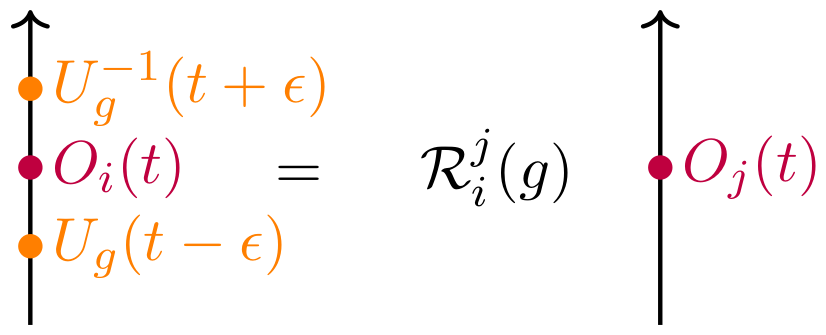
\includegraphics[width=0.32\linewidth]{figures/figure-1.png}
  % [原文图注为空]
  \caption{}
  \label{Fig:0FormQM}
\end{figure}

那么“拓扑的”究竟指什么？既然 $U_g$ 与哈密顿量对易，它就可以沿时间轴移动，只要“障碍”$\{ O_i(t)\}$ 不挡路。这一拓扑性质在更高维的例子中会表现得更为明显。

\begin{example}[$M^d$ 中的 0-形式对称性]
    为推广上例，把 0-形式对称性（0-form symmetry）定义为由支撑在 $M^{(d-1)}\subset M^d$ 上的一组幺正拓扑算符生成，且满足 $U_g(M^{(d-1)})U_{g'}(M^{(d-1)}) = U_{gg'}(M^{(d-1)})$。其作用定义为
    \[ U_g(S^{d-1}) O_i(p) =  \mathcal{R}_i^j(g) O_j(t) \ ,  \]
    其中 $p$ 是 $S^{d-1}$ 内部的一点。
\end{example}

初看之下这似乎奇怪：前例中的“$U_g^{-1}$”部分不见了；但它实际上只是上例的推广。$1+1$ 维情形的图示理解见图~\ref{Fig:1FormQM}，更高维可想象类似的图景。

\begin{figure}[htbp]
  \centering
  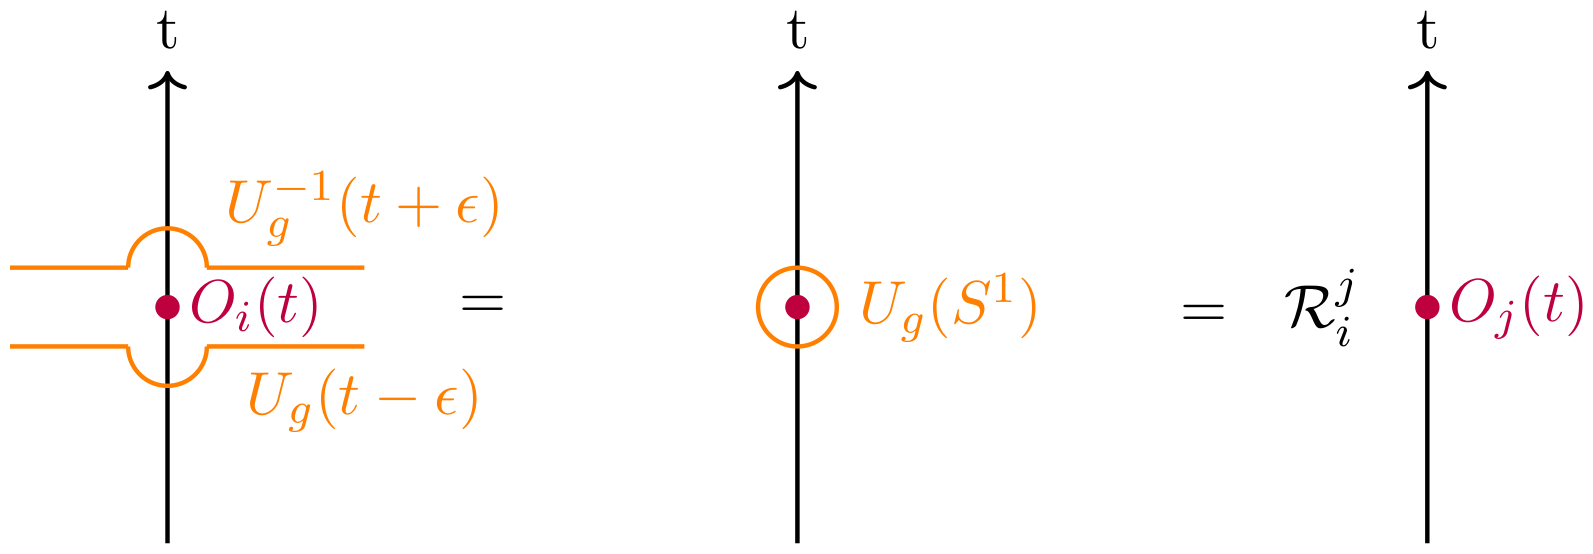
\includegraphics[width=0.62\linewidth]{figures/figure-2.png}
  % [原文图注为空]
  \caption{}
  \label{Fig:1FormQM}
\end{figure}

\begin{yizhu}上例到本例中“$U_g^{-1}$ 消失”只是画法的变化，并非定义改变：量子力学里 $U_g(t-\epsilon)$ 与 $U_g^{-1}(t+\epsilon)$ 是时间轴上夹住 $O_i(t)$ 的一对点插入，而 0-形式对称性把这对点“接”成一个闭合的 $S^{d-1}$（图~\ref{Fig:1FormQM} 左端即用一个环绕点算符的 $S^1$ 表示），闭合面上只剩一次插入，故作用律中不再显式出现逆算符。核对图~\ref{Fig:1FormQM} 时应看出：橙色圆环在时间轴上跨接并包住了原来上下两个插入点，于是 $\mathcal{R}(g)\mathcal{R}(g^{-1})=1$ 已在环内被用掉。\end{yizhu}

\begin{example}[$M^d$ 中的电磁学]
考虑 $d$ 维纯麦克斯韦理论中的 $U(1)$ 守恒流，
\[ \dd *F = j \]
于是
\[ U_g(M^{(d-1)}) = g^{\int_{M^{(d-1)}} j}  = \exp(i\alpha \int_{M^{(d-1)} } j ) \]
其中 $g = \exp(i\alpha)\in U(1)$ 是对称群的一个群元\footnote{事实上，前一情形中所说的 $U(1)$ 其实对应于 $U(1)$ 规范对称性的整体部分，即 $\alpha$ 与时空无关时的那一部分。}。
\end{example}

% ==== 原文 PDF 第 8 页 ====
若把 $M^{(d-1)}$ 取为一个时间切片，则 $\int_{M^{(d-1)} } j$ 就是该体系的总电荷。这一算符为何是拓扑的？这由 Stokes 定理给出。考虑对 $M^{(d-1)}$ 作一个小形变（小到没有点电荷穿过），记其为 $M^{(d-1)\prime}$，则
\[  \int_{M^{(d-1)}} j -  \int_{M^{(d-1)\prime}} j   = \int_{\partial D} j = \int_{D} \dd j = 0  \ , \]
其中 $D$ 是被形变部分所围的体积。$U_g$ 算符确实是拓扑的。

\begin{yizhu}记号预警：$\dd *F = j$ 中的 $j$ 是 $(d-1)$-形式，即电流 1-形式 $j_\mu$ 的 Hodge 对偶 $\star j$，而不是 $j_\mu$ 本身；因此 $\int_{M^{(d-1)}}j$ 是通量型积分。对照后文 (2.18) 写成 $\frac{1}{e^2}\dd *F = *j_E$ 就看得更清楚：那里右端显式带上星号，正是为了把 1-形式的电流 $j_E$ 与 $(d-1)$-形式的 $j$ 区分开。若把两处的 $j$ 混为一谈，会连带读错 (2.6) 与 (2.18) 中 $1/e^2$ 的归一化。\end{yizhu}

\subsection{高形式对称性}\label{sec:higher-form}

用拓扑算符的语言，向高形式对称性的推广是直截了当的：只需把与对称性算符相应的余维 $1$ 子流形（即 $d-1$ 维子流形）换成余维 $(p+1)$ 的流形，并把局域算符换成定义在 $p$ 维子流形上的对象（$p$ 维延展算符）。如此，拓扑算符记为 $U_g(M^{d-p-1})$，对象记为 $V(C^{p})$，则对称性对对象的作用为
\be
U_g(M^{d-p-1})V_i(C^p) = R_i {}^{j}(g) V_j(C^p) \ ,
\ee
前提是环绕数（linking number）$\langle M^{d-p-1},C^{p} \rangle = 1$。这里环绕数可直观地理解为两个子流形（维数之和为 $d-1$）在拓扑上相互缠绕而互不相交的方式；更清晰的定义是
\be
\langle M^{d-p-1},C^p \rangle = {\rm Int}(X^{d-p}, C^p) = {\rm Int}(M^{d-p-1}, Y^{p+1}) \ ,
\ee
其中 $\partial X^{d-p} = M^{d-p-1}$、$\partial Y^{p+1} = C^{p}$ 表明 $X^{d-p}$ 与 $Y^{p+1}$ 分别以 $M^{d-p-1}$ 与 $C^{p}$ 为边界，${\rm Int}$ 表示交点数（intersection number）。该公式的直观含义见下图。

\begin{center}
    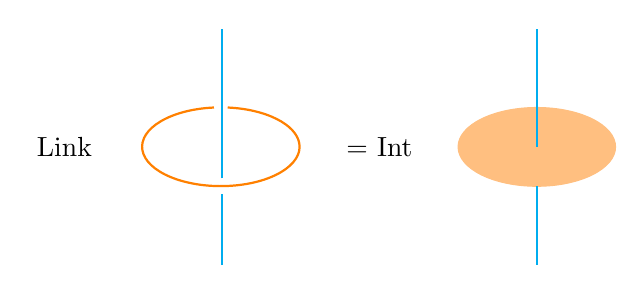
\begin{tikzpicture}
    \draw[thick, cyan] (-2,0.1)--(-2,2);
    \draw[thick, cyan] (-2,-1)--(-2,-0.1);
    \draw[thick, orange] (-2.1,1) arc (-265:85:1 and 0.5);
    \node[] at (0,0.5) {=  Int};
    \node[] at (-4,0.5) {Link};

    \filldraw[orange!50] (2.0,0.5) ellipse (1 and 0.5);
    \draw[thick, cyan] (2,0.5)--(2,2);
    \draw[thick, cyan] (2,0)--(2,-1);
    \end{tikzpicture}
\end{center}

\begin{yizhu}“相链”判据的两点提醒。其一，维数配平：$\dim M^{d-p-1}+\dim C^{p}=d-1$，故二者在 $d$ 维时空中一般不交；引入以 $M^{d-p-1}$ 为边界的 $X^{d-p}$ 后 $\dim X^{d-p}+\dim C^{p}=d$，横截相交为有限个点，故 $\langle M,C\rangle$ 等于交点数——这正是图中“Link $=$ Int”的含义。其二，交点数带定向符号：原文写 $\langle M^{d-p-1},C^{p}\rangle = 1$，使用时应理解为 $|\langle\cdot\rangle|=1$，相位 $\mathrm{e}^{in\alpha}$ 的符号取决于两子流形定向的选取。此外，原文 “The intuition for formula is” 一句在 PDF 中只接一幅图、未给文字说明，属原文行文疏略。\end{yizhu}

当然，作为作用在该体系上的对称群的表示，应当有
\be
U_g(M^{d-p-1})U_{g'}(M^{d-p-1})=U_{gg'}(M^{d-p-1}) \ .
\ee

\begin{yizhu}[原文疑误]此处有两处与源码/PDF 有关的细节。其一，源码把延展对象写作 $V_(C^{p})$（下划线直接接括号，TeX 会把它排成下标 $(C^{p})$），而 PDF 第 8 页实际排为 $V(C^{p})$；本译本从 PDF，恢复为 $V(C^{p})$。其二，本段原文作 “as a representation of the symmetric group”，按上下文（对称性算符的乘法律 $U_gU_{g'}=U_{gg'}$）应为 “symmetry group”；中文里两词都译作“对称群”，译文不显差别，但核对英文时勿误读为置换群 $S_n$。\end{yizhu}

接下来论证：若 $p>0$ 且时空拓扑平凡，则高形式对称性总是\textbf{阿贝尔的}。用拓扑算符的语言，这一论证几乎是显然的：
% ==== 原文 PDF 第 9 页 ====
设有两个余维 $\ge 2$ 的算符，就可以在时空中把二者作拓扑互换而没有任何障碍。图示情形见图~\ref{Fig:Abelian}。但在 $p=0$ 的情形无法作这样的互换，因为两个拓扑算符 $U_g$ 支撑在不同的时间切片上，它们一般可以不对易。

\begin{figure}[htbp]
  \centering
  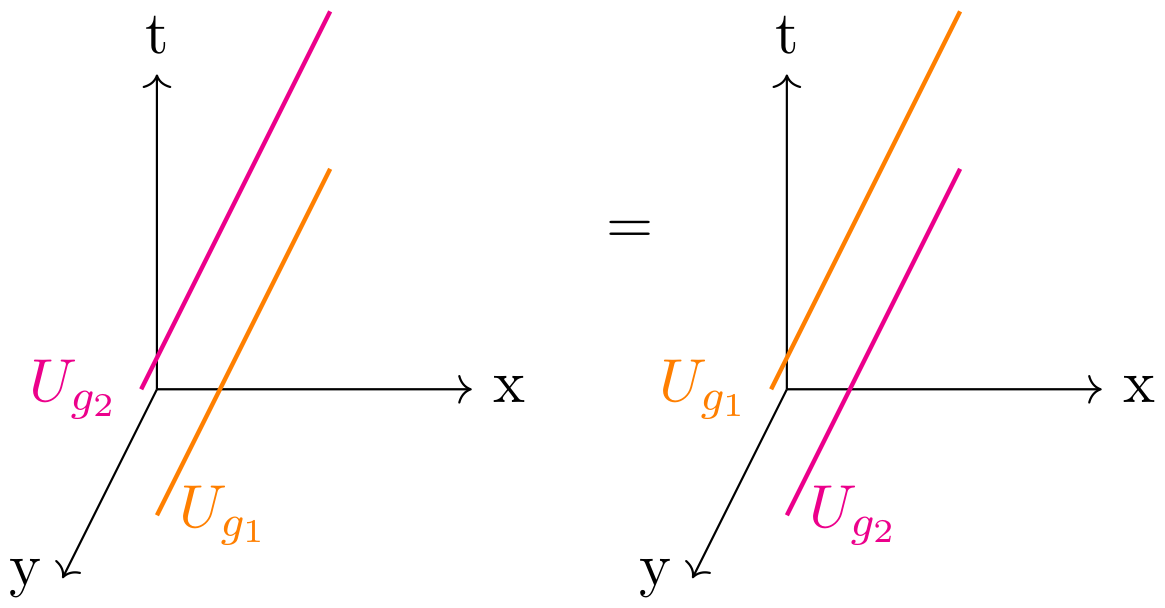
\includegraphics[width=0.46\linewidth]{figures/figure-3.png}
  \caption{在 $p>0$ 时交换拓扑算符。（原文 Figure~3，PDF 第 9 页）}
  \label{Fig:Abelian}
\end{figure}

\subsubsection{例：麦克斯韦理论}\label{subsec:Maxwell}

考虑 4 维纯 $U(1)$ 麦克斯韦理论，其作用量为
\be
S = \frac{1}{4e^2} \int {\rm d}^4 x \ F_{\mu\nu}F^{\mu\nu}
\ee
其中 $F_{\mu\nu} = \partial_\mu A_\nu- \partial_\nu A_\mu$，或等价地，$F = \frac{1}{2} F_{\mu\nu}{\rm d}x^\mu \wedge {\rm d}x^\nu = {\rm d}A $。众所周知，该理论具有 $U(1)_E \times U(1)_M$ 1-形式对称性。

下面说明 $U(1)_E$ 是 1-形式对称性：它由 $4-1-1=2$ 维拓扑算符生成，并作用在 1 维对象上。电的 $U(1)_E$ 对称性由拓扑算符
\be
\label{U1-UE}
U_E (S) = \exp(i\alpha Q_E(S))
\ee
生成，其中 $Q_E(S)$ 是 $S$ 所围的总电荷，即
\be
Q_E(S) = \frac{1}{e^2}\int_S *F = \frac{1}{e^2}\int_S \frac{\epsilon_{\mu\nu\rho\sigma}}{2!\cdot 2!}F^{\mu\nu} {\rm d}S^{\rho\sigma} \sim  \int_S \vb{E}\cdot \vb{{\rm d}S}\,.
\ee
该算符确实是拓扑的：由运动方程 ${\rm d}*F = 0 $，不碰到电荷的形变不会改变该算符。

那么算符所作用的对象是什么？答案是威尔逊圈（Wilson loop）。对给定的圈 $\gamma:[0,1]\to M, \gamma(1)=\gamma(0)$，威尔逊圈算符为
\be 
W_n(\gamma) = \exp(i n  \oint_\gamma A_\mu {\rm d}x^\mu )  = \exp(i n \int_\gamma A )\,. 
\ee
% ==== 原文 PDF 第 10 页 ====
拓扑算符 (\ref{U1-UE}) 对威尔逊圈的作用为（证明稍后在命题~\ref{Prop:1} 中给出）
\be
\expval{U_E(S) W_n(\gamma)} = \exp(in\alpha \expval{S,\gamma}) \expval{W_n(\gamma)}\,.
\ee

\textbf{注}：
\begin{enumerate}
\item 在威尔逊圈的定义中 $n\in \bbZ$。量子化的原因在于：在大规范变换 $A_\mu\mapsto A_\mu + \partial_\mu \epsilon$ 下，
    \[ \oint_\gamma \partial_\mu \epsilon {\rm d}x^\mu  = 2\pi k \quad \ k\in \bbZ\,, \]
    其中 $k$ 是绕数（winding number）。因此只有当 $n\in\mb{Z}$ 时，威尔逊圈才是规范不变的。
    
    \item 拓扑算符对威尔逊圈的这一作用，可等价地看作把 $A$ 平移一个平坦联络 $\lambda$（平坦指 ${\rm d}\lambda = 0$），即
    \be
    \oint_\gamma \lambda = \alpha \expval{S,\gamma}\,.
    \label{Eq:intlambda}\ee
    还应注意，该积分在 $\gamma$ 作小形变下不变。

    注意：即使 $\lambda$ 是平坦的，它也不能写成局域规范变换 $\lambda=d\epsilon$，否则对称性作用就是平凡的。
    
\end{enumerate}

现在转向与电对称性对偶的磁 $U(1)_M$ 对称性。这里的窍门很简单：给每样东西都配上 Hodge 星号 $*$。显然有
\be
U_M (S) = \exp(i\alpha Q_M(S))\,,
\ee
\be Q_M(S) = \frac{1}{2\pi}\int_S F = \frac{1}{4\pi}\int_S F_{\mu\nu} {\rm d}S^{\mu\nu} \sim  \int_S \vb{B}\cdot \vb{{\rm d}S} \,.
\ee
该算符是拓扑的，因为 ${\rm d}F = {\rm d^2}A = 0$。为构造威尔逊线的对偶版本，定义 $\tA$ 使得 ${\rm d}\tA = *\dd A $。于是 't Hooft 圈定义为
\be 
T_n(\gamma)  = \exp(i n \oint_\gamma \tA) = \exp(i n \oint_\gamma \tA_\mu \dd x^\mu)\,.
\ee
当然，$U_M$ 算符对 't Hooft 圈的作用为
\be
\expval{U_M(S) T_n(\gamma)} = \exp(in\alpha \expval{S,\gamma}) \expval{T_n(\gamma)}\,.
\ee
这也可以解释为把 $\tA$ 平移一个平坦联络。

\begin{prop}
\label{Prop:1}
\[ \expval{U_E(S) W_n(\gamma)} = \exp(in\alpha \expval{S,\gamma}) \expval{W_n(\gamma)}  \]
\end{prop}
% ==== 原文 PDF 第 11 页 ====
\begin{proof} 
\be {\rm L.H.S} = \int \mathscr{D}[A] \exp{iS + \frac{i\alpha}{e^2}\int_S *F + in \oint_\gamma A} \ee
这里的想法是对 $A$ 作一个平移：在此平移下测度 $\mathscr{D}[A]$ 不变，而指数上的各项只改变一个全导数项（在时空拓扑平凡的情形下无贡献），外加一个涉及环绕数的项。考虑
\begin{align*}
    \int_S *F &= \int_{V_S(\partial V_S = S)} d*F = \int_{V_S} \frac{\epsilon_{\nu\rho\sigma\tau}}{3!} \partial_\mu F^{\mu\nu} \dd v^{\rho\sigma\tau}\\
    &= \int \dd^4 x \ \partial_\mu F^{\mu\nu} J_\nu(V_S) = -\int\dd^4 x \ F^{\mu\nu} \partial_\mu J_\nu(V_S)
\end{align*} 
其中定义
\[ J_\nu(V_S) = \int_{V_S} \frac{\epsilon_{\nu\rho\sigma\tau}}{3!} \delta^4(x-y) \dd v^{\rho\sigma\tau}(y)\,. \]
可以看到这些项如何在 $A-\alpha J(V_S)$ 附近展开，相应结果为
\begin{align}
    W_n(\gamma,A) &= W_n(\gamma,A-\alpha J(V_S)) \exp(in\oint_\gamma J(V_S)) \\
    S[A] &= S[A-\alpha J(V_S)] + \frac{\alpha}{e^2} \int \dd^4 x \ \pmu J_\nu(V_S) \Fmn \ (+ {\rm higher\  derivative \ terms\ in\ }J_\mu) \ .
\end{align}

$J_\mu$ 中的高阶导数项不依赖于 $A$，因此作为归一化因子被略去。

最后，在作平移 $A\mapsto A-\alpha J(V_S)$ 之后，得到
\be
\expval{U_E(S) W_n(\gamma)} = \exp(in\alpha \oint_\gamma J(V_S)) \expval{W_n(\gamma)} \ .
\ee
由涉及交点数的定义可得
\[\oint_\gamma J(V_S) = \expval{S,\gamma}\,.\]

\end{proof}

\subsubsection{例：带荷物质的 $U(1)$ 规范理论}

现在给麦克斯韦理论加上带荷物质 $\{ \phi_i\}$，其电荷为 $q_i \in \bbZ$，即 $R_{q_i} (e^{i\alpha}) = e^{iq_i\alpha}$；同时定义正整数 $N = {\rm g.c.d}(q_i)$。

本情形的主要差别在于：$U(1)_E$ 的对称性流 $*F$ 不再守恒，取而代之的是
\be \frac{1}{e^2} \dd *F = *j_E \ , \ee
% ==== 原文 PDF 第 12 页 ====
其中 $j_E$ 是通常的电电流 1-形式。然而，若仍要求算符
\be U_E(e^{i\alpha}, S) = \exp(\frac{i\alpha}{e^2} \int_S *F) \ , \ee
是拓扑的，就要求 $S$ 的任意形变都保持不变，见图~\ref{fig:VS}。

\begin{figure}[htbp]
  \centering
  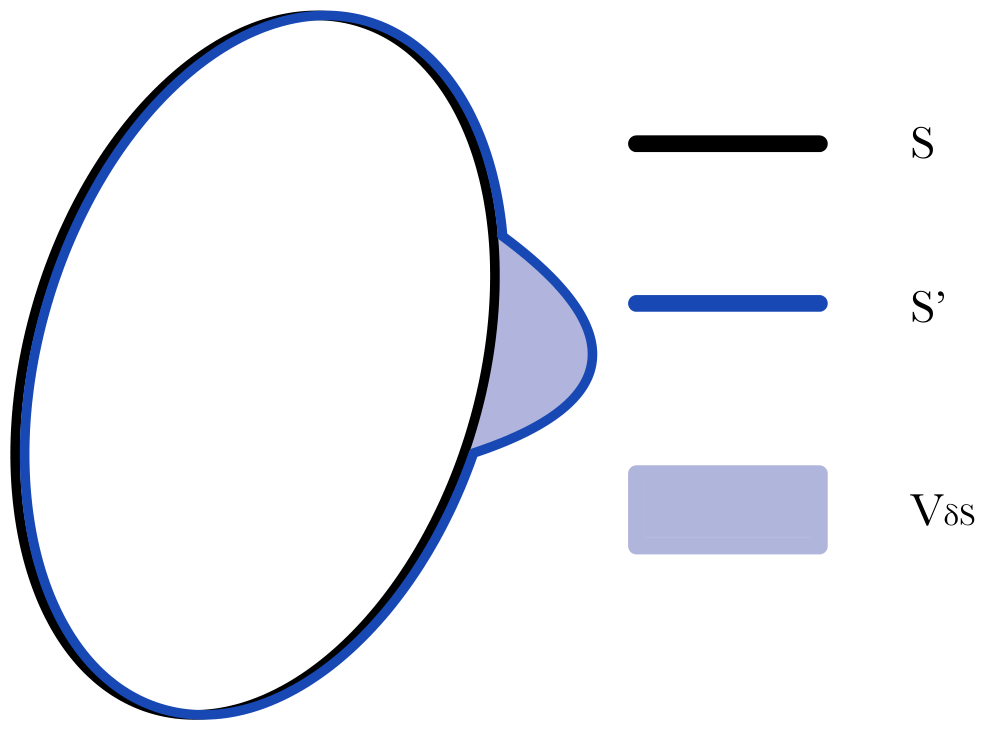
\includegraphics[width=0.39\linewidth]{figures/figure-4.png}
  \caption{本图展示从闭流形 $S$ 到 $S'$ 的形变：二者分别用黑色粗线与蓝色粗线标出。两个曲面会围出一个体积，该体积上的通量积分给出相应两个拓扑算符之差，见式~(2.20)。（原文 Figure~4，PDF 第 12 页）}
  \label{fig:VS}
\end{figure}

\be\ba 
U_E(e^{i\alpha}, S) &= U_E(e^{i\alpha}, S') \\
\Rightarrow \exp(\frac{i\alpha}{e^2}\int_{V_{\delta S}} \dd * F ) &= \exp(i\alpha\int_{V_{\delta S}} \ * j_E ) = 1 \quad \ptl V_{\delta S} = S \cup \overline{S'} \label{eq:VS}
\ea\ee

电荷量子化给出 $\int_{V_S} \ *j_E \in N\bbZ $，因此为满足 (\ref{eq:VS})，要求 $\alpha \in 2\pi \bbZ_N / N$。

\begin{yizhu}记号提醒：$\alpha \in 2\pi \bbZ_N / N$ 是原文的混写，字面上把群 $\mathbb{Z}_N$ 放到了整数集的位置。其实际含义是 $\alpha = 2\pi k/N$（$k\in\mathbb{Z}$，且 $\alpha$ 只定义到模 $2\pi$），即 $\alpha$ 取 $\mathbb{Z}_N$ 的 $N$ 个离散值；若读成“$\mathbb{Z}_N$ 的分数”便得不到对称性破缺到 $\mathbb{Z}_N$ 的结论。可与下文例~5 的结果对照：那里 $D=\mathrm{diag}(3,1)$，电对称性恰好破缺为 $\mathbb{Z}_3$。\end{yizhu}

因此，$U(1)_E$ 电 1-形式对称性群破缺为 $\bbZ_N$ 子群。还值得注意的是，在不包含磁单极子时，$U(1)_M$ 保持不变。

这一框架可以推广到带荷物质场 ${\phi_i}$ 的 $U(1)^r$ 规范理论。场 $\phi_i$ 在第 $j$ 个 $U(1)$ 对称性下的电荷为 $q_{i,j}\in\bbZ$。为计算对称性破缺，把荷矩阵记为 $Q = (q_{i,j})$，其中 $Q$ 不必是方阵。
% ==== 原文 PDF 第 13 页 ====
Smith 标准形分解（Smith normal decomposition）给出如下结果：
\be
\label{SmithDecomp}
U Q V = D = \begin{pmatrix}
d_1 &     &        &     &   &   &   \\
    & d_2 &        &     &   &   &   \\
    &     & \ddots &     &   &   &   \\
    &     &        & d_k &   &   &   \\
    &     &        &     & 0 & 0 & 0 & \cdots \\
    &     &        &     & 0 & 0 & 0 & \cdots
\end{pmatrix}\,.
\ee

这里 $U$ 与 $V$ 是元素为整数的可逆方阵。由此得到的 1-形式对称性为 $(\bigoplus_{i=1}^k \bbZ_{d_i})\oplus U(1)^{r-k} $。磁 1-形式对称性仍是 $U(1)_M=U(1)^r$。

\begin{yizhu}Smith 标准形 $UQV=D$ 的读法：$U,V$ 是整系数可逆方阵（$\det U=\pm1$、$\det V=\pm1$），左乘相当于重定义 $U(1)^r$ 规范荷的基底、右乘相当于重定义物质场基底，故不改变物理。对角元中只有 $d_i>1$ 的部分给出离散因子 $\mathbb{Z}_{d_i}$，$d_i=1$ 的因子不贡献；而 $Q$ 的秩之外的方向不被任何物质场带荷，剩下连续因子 $U(1)^{r-k}$。若 $Q$ 为满秩方阵，则 $\prod_i d_i=|\det Q|$，可用来快速验算：例如 (2.22) 的 $\det Q=3$ 正给出 $\mathbb{Z}_3$。\end{yizhu}

\begin{example}[具有 $\mb{Z}_3$ 电 1-形式对称性的理论]
作为例子，考虑 $U(1)^2$ 规范理论，其物质场的电荷为 $\phi_1=(2,-1)$、$\phi_2=(-1,2)$。
\end{example}

于是荷矩阵为
\be
Q=\bp 2 & -1\\-1 & 2\ep\,.
\ee
经过 Smith 标准形分解得到 $D=\rm{diag}(3,1)$，因此电 1-形式对称性破缺为 $\mb{Z}_3$ 子群。

事实上，这恰好是纯 $SU(3)$ 规范理论的库仑相（Coulomb phase）。

\subsubsection{4 维非阿贝尔规范理论}

另一类众所周知的例子是非阿贝尔规范理论，读者可参阅 David Tong 的规范理论讲义~\cite{TongGauge}。为简单起见，考虑规范群为 $G$ 的纯杨–米尔斯理论。

对 $G = SU(N)$，$\bbZ_N$ 是由 $SU(N)$ 的中心生成的 1-形式电对称性，它作用在对此对称性带荷的威尔逊圈上。

下面讨论 $S^1\times\mb{R}^3$ 上的有限温度体系，其中欧氏时间圆满足 $x^0\sim x^0+\beta$。$\mb{Z}_N$ 1-形式中心对称性由函数的等价类 $[h_k]=\{h_k(x^\mu)\in SU(N), h_k(x^\mu)\sim g(x^\mu)h_k(x^\mu)g^{-1}(x^\mu)\}$ 定义，该等价类到 $SU(N)$ 的中心为止是周期的：$h_k(x^0=\beta)=e^{2\pi k/N}h_k(x^0=0)$。它对 $A$ 的作用为
\be
A\rightarrow h_kAh_k^{-1}+h_kdh_k^{-1}\,,
\ee
该作用在局域算符上是平凡的，但在 Polyakov 圈
\be
P_R=\text{tr}_R(\mathcal{P}\exp\left(\oint_{S^1}A^0\right)
\ee
上非平凡：
\be
P_R\rightarrow P_R e^{\frac{2\pi i k n_R}{N}}\,.
\ee
% ==== 原文 PDF 第 14 页 ====
其中 $R$ 是 $SU(N)$ 的表示，它定义了威尔逊圈（Polyakov 圈）；$n_R$ 称为“$N$-性”（N-ality），等于 $R$ 的杨图中方框总数模 $N$。

$\mb{Z}_N$ 1-形式对称性的这一作用也适用于一般的威尔逊圈：
\be
\ba
U_{k(\in \bbZ_N)}(S^2) W_R(\gamma) &= W_R(\gamma) \Big[A + \frac{2\pi k}{N} I \Big] \quad \expval{S^2 ,\gamma} = 1\cr
&=e^{\frac{2\pi ik n_R}{N}}W_R(\gamma)\,.
\ea
\ee

在 $G = PSU(N) = SU(N)/\bbZ_N$ 的情形，体系表现出作用在 't Hooft 圈上的 $\bbZ_N$ 磁对称性，原因在于 $\pi_1(PSU(N))=\mb{Z}_N$~\cite{TongGauge}。下面的描述可以说明这一点。考虑纯空间中的磁单极子（在时空中即 't Hooft 线）；吴–杨磁单极子构造告诉我们，把空间分为北/南半球后，规范势为
\be\ba
A_N = &B_0 \frac{1+\cos(\theta)}{2 r^2} \dd \phi \\
A_S = &B_0 \frac{-1+\cos(\theta)}{2 r^2} \dd \phi \\
\ea\ee
而赤道处的拼接条件为
\be \exp(i B_0\phi) =  \exp(i B_0(\phi+2\pi) )\Rightarrow \exp(2\pi i B_0 ) = I_{PSU(N)} \ee
这样的 $B_0$ 选择由 $\pi_1(PSU(N)) = \bbZ_N$ 分类。

我们指出：在 $SU(N)$ 理论中存在中心 $\bbZ_N^{(1)}$ 对称性，但没有这种磁对称性，因为 $\pi_1(SU(N)) = 0$。而在 $PSU(N)$ 理论中没有中心对称性（其中心平凡），但有磁 $\bbZ_N^{(1)}$ 对称性。这一关系可以推广，见~\cite{Brennan:2023mmt}。

更一般地说，在规范李代数为 $\mathfrak{su}(N)$ 的纯杨–米尔斯理论中，可以用荷 $(n_E,n_M)\in \bbZ_N\times \bbZ_N$ 对圈算符分类。荷为 $(n_E,n_M)$ 与 $(n_E',n_M')$ 的两个这类算符相互局域（从而可以共存），当且仅当它们满足狄拉克量子化条件
\be
n_E n_M'-n_M n_E'=0\quad (\text{mod}\ N)\,.
\ee
这样一组互局域算符的选取称为\textbf{极化}（polarization）。例如，若选取全部威尔逊圈作为互局域算符集合，则该规范理论的整体形式是 $G=SU(N)$ 规范理论；相反，若选取全部 't Hooft 圈，则整体形式是 $G=PSU(N)$ 规范理论。当然，当 $N$ 不是素数时，还可以有介于两者之间的情形。

% ==== 原文 PDF 第 15 页 ====
选定极化之后，该理论称为\textbf{绝对理论}（absolute theory），其配分函数良定义；否则一般称为\textbf{相对理论}（relative theory），只有配分向量。配分向量的概念最早是在 6 维 (2,0) 理论及其环面紧致化的语境中引入的，那里存在互不局域的双子（dyonic）带荷算符，详见~\cite{Witten:2009at,Freed:2012bs,Tachikawa:2013hya}。

% ============================================================
% 片段：s02b  对应原文 section2.tex 第 355--646 行；PDF 第 15--24 页
% 内容：§2 Higher-Form Symmetry（2.3 Gauging Higher-Form Symmetry；2.4 Symmetry Trifecta）
% 译者：t-s02b   审校状态：初稿
% ============================================================

% ==== 原文 PDF 第 15 页 ====

\subsection{高形式对称性的规范化}\label{sec:gauging}

一个近乎古老却又历久弥新的问题是：什么是规范化？它通常指把某个整体对称性变成规范对称性的操作。但什么是规范对称性？在某些说法中，它指的是依赖于时空的对称性，不过这会有一些限制；例如，若不放弃光滑性，如何能让一个离散对称性依赖于时空、同时又区别于整体对称性？更好的理解是对规范场的所有可能“构型”求和，从而使规范变换确定地成为冗余；关于这些表述，我们将在第~\ref{sec:three}~节中说得更为明确。本节中，除非另有说明，$p$-形式对称性群 $G^{(p)}$ 是阿贝尔的。我们把这种对称性的背景 $(p+1)$-形式规范场记为 $A^{(p+1)}$。

更准确地说，规范化有两种等价的视角：
\begin{enumerate}
    \item 对算符 $U_g(M^{d-p-1})$ 的所有可能插入求和；
    \item 把 $A^{(p+1)}$ 提升为动力学规范场，然后对 $A^{(p+1)}$ 的所有构型作积分（求和）。
\end{enumerate}
特别地，在规范化有限阿贝尔群的情形，有如下命题：
\begin{prop}
\label{prop:gauge}
    在对理论 $Z[A^{(p+1)}]$ 的有限阿贝尔对称性 $G^{(p)}$ 作规范化之后，规范化后的理论 $Z'$ 会显现一个新的对称性 $\hat{G}^{(d-p-2)}$，其中 $\hat{G}\equiv {\rm Hom}_{\rm Grp}(G,U(1))$ 是 $G$ 的 Pontryagin 对偶。规范化后的理论具有配分函数
    \be Z'[\hat{A}^{(d-p-1)}] = \sum_{[A^{(p+1)}] \in H^{(p+1)}(M^d; G^{(p)})} Z(A^{(p+1)}) \exp(2\pi i \int_{M^d} \expval{\hat{A}^{(d-p-1)},A^{(p+1)}}  ) \ , \ee
    其中 $\expval{}$ 是群层面的内积。当群 $G^{(p)}$ 连续时，$\expval{}$ 对应取值于 $\Hat{\mathfrak{g}}$ 的元素作用在取值于 $\mathfrak{g}$ 的元素上的楔积。若 $G^{(p)}$ 离散，$\expval{}$ 应解释为取值于 $\Hat{G}$ 的元素作用在取值于 $G$ 的元素上的杯积。
\end{prop}

\begin{yizhu}
(2.30) 式的求和不是对规范场构型的泛函积分，而是对\textbf{上同调类} $[A^{(p+1)}]\in H^{(p+1)}(M^d;G^{(p)})$ 求和（即只对平坦背景求和），这是“有限阿贝尔群”这一前提的直接后果，也是后文能用上同调与杯积语言的原因；对连续群，该求和须换成对联络的积分，命题的表述要另行处理。另须核对两处形式次数：规范化的对象是 $p$-形式对称性，其背景场是 $(p+1)$-形式，而规范化后出现的是 $d-p-2$ 形式的对偶对称性，其背景场为 $(d-p-1)$-形式——这正是 (2.30) 左端写 $\hat{A}^{(d-p-1)}$ 的缘由。所谓“再规范化一次回到原理论”，依赖的是 Pontryagin 对偶 ${\rm Hom}({\rm Hom}(G,U(1)),U(1))=G$，它对有限阿贝尔群成立；$\expval{}$ 在连续/离散两种情形分别取楔积与杯积，勿混用。
\end{yizhu}

\begin{proof}
    在开始证明之前，先体会一下该定理的直观。按朴素的看法，对具有 0-形式对称性的理论作规范化，应当相当于把希尔伯特空间投影到物理的希尔伯特空间，但并不尽然。该投影是非可逆的，而为了保留%
% ==== 原文 PDF 第 16 页 ====
表示的信息，我们可以插入一条威尔逊线（回忆一下，威尔逊线由所选表示标记）。

    因此这里我们也照此办理。耦合项
    \[\exp(2\pi i \int_{M^d} \expval{\hat{A}^{(d-p-1)},A^{(p+1)}}  ) \ , \]
    可以看作耦合了一个离散通量。依照此前的方法，理论 $Z$ 中的对称性算符应由该离散通量构造（它是威尔逊线的更高维版本）\cite{Schafer-Nameki:2023jdn}
    \be D(M^{d-p-1} ) = \exp(i\int_{M^{d-p-1}} \hat{A}^{(d-p-1)}) \ . \ee
    但有什么地方不对：$\hat{A}^{(d-p-1)}$ 取值于 $\Hat{G}$ 而非 $G$！这里的正确理解是：\textbf{融合规则仍是 $G$ 的乘法}，这通过把算符正确写成
    \be D(\rho, M^{d-p-1}) = \rho\Big( \exp(i\int_{M^{d-p-1}} \hat{A}^{(d-p-1)})\Big) \ , \ \rho\in {\rm Rep}(\Hat{G}) = G \ .  \ee
    来实现。于是对称性算符的融合规则为
    \be D(\rho_1 ,M ) \otimes D(\rho_2,M) = D(\rho_1\otimes \rho_2 ,M)   \ee
    它正确地以 $G$ 的乘法作为融合规则。\footnote{感谢 Ruizhi Liu 对这部分的有益讨论。}

    类似地，对于规范化后的理论 $Z'$，对称性算符构造为
    \be D'(\rho', M^{p+1}) = \rho'\Big( \exp(i\int_{M^{p+1}} A^{(p+1)}) \Big)\ , \ \rho'\in {\rm Rep}(G) = \Hat{G} \ . \ee
    既然对称性算符已构造出来，我们就可以合理地说 $Z'$ 理论具有 $\Hat{G}^{(d-p-2)}$ 对称性。
\end{proof}

\begin{yizhu}
证明中“但有什么地方不对”这一步是全段的枢纽，作者只用一句话带过，其实质是：$\hat{A}^{(d-p-1)}$ 是 $\Hat{G}$ 值的，故 $\exp(i\oint\hat{A})$ 本身并不按 $G$ 的元素标记，直接用它会得到错误的融合规则。修补办法是把 $\Hat{G}$ 的表示（特征标）$\rho\in{\rm Rep}(\Hat{G})$ 复合上去；由 Pontryagin 对偶 ${\rm Rep}(\Hat{G})=G$，$\rho_1\otimes\rho_2$ 恰好对应 $G$ 中的乘法 $g_1g_2$，于是融合规则 (2.33) 自动成立。反过来，对偶理论 $Z'$ 的算符用 $\rho'\in{\rm Rep}(G)=\Hat{G}$ 构造，两套算符的形式完全对称——这正是“再规范化一次回到原理论”的来源。此处不必也不应把 $\rho$ 理解成矩阵的迹：它只承担“把 $\Hat{G}$ 值翻译成 $G$ 值”的角色。
\end{yizhu}

作为推论，我们实际上可以对 $\hat{G}^{(d-p-2)}$ 再作一次规范化，从而回到原来的理论。这只是一个简单的练习：只需注意到 ${\rm Hom}( {\rm Hom}(G,\U(1)) , U(1) ) = G$ 以及 $d-(d-p-2)-2 = p$。

\subsubsection{$p$-形式对称性的 't Hooft 反常}

然而，在某些情形下规范化无法完美实施，可能存在障碍，我们称之为 't Hooft 反常。它是规范变换导致理论配分函数发生改变的现象。
% ==== 原文 PDF 第 17 页 ====
也就是说，若取 $\delta_\lambda A$ 为背景规范场的一般变换\footnote{对无穷小规范变换，它称为\textbf{局域反常}；对大规范变换，它称为\textbf{整体反常}。}，
\be Z(A + \delta_\lambda A) = \exp(2\pi i \int_{M^d} I_d)\cdot  Z(A) \  \ee
其中 $I_d$ 是由规范场构成的 $d$-形式。当然，只有当这样的相位因子 $2\pi i \int_{M^d} I_d$ 无法被 $d$ 维作用量中规范不变的局域抵消项消去时，我们才说该系统具有 't Hooft 反常。

处理该问题的一个标准做法是通过下降公式（descent formula）。其想法是找一个规范不变的客体来描述反常。下降公式为
\be
\ba
\dd I_d = \delta_\lambda I_{d+1} \ , \ \dd I_{d+1}  = I_{d+2} \cr
Z(A + \delta_\lambda A) = \exp(2\pi i \int_{M^{d+1}} \delta_\lambda I_{d+1})\cdot  Z(A)
\ea
\ee
其中 $\ptl M^{d+1} = M^d $。$I_{d+1}$ 是 $(d+1)$-形式 't Hooft 反常多项式，$I_{d+1} $ 是规范不变的 $(d+2)$-形式。

\begin{yizhu}[原文疑误]
(2.36) 之后一句原文（源码第 410 行，PDF 第 17 页同）为“$I_{d+1}$ 是 $(d+1)$-形式 't Hooft 反常多项式，$I_{d+1}$ 是规范不变的 $(d+2)$-形式”：第二个 $I_{d+1}$ 显然应为 $I_{d+2}$（否则与 $(d+2)$-形式自相矛盾，也与上一行 $\dd I_{d+1}=I_{d+2}$ 冲突）。此处照原文保留符号，读者应按 $I_{d+2}$ 理解。顺带说明这条下降链的标准读法：$I_{d+2}$ 是闭的不变多项式，$I_{d+1}$ 是其陈–西蒙斯型“势”，$\delta_\lambda I_{d+1}=\dd I_d$ 给出反常的局域形式；作者把两条关系并排写成一个公式，读取时不要误以为 $\delta_\lambda I_d$ 也参与同一等式。
\end{yizhu}

这给出“反常流入”（anomaly inflow）机制的线索：$d$ 维的 QFT 可以与 $(d+1)$ 维的 QFT 耦合。一个一般的构造是：如上定义、带有 't Hooft 反常的 $M^d$ 上的 QFT，可以与 $M^{d+1}$ 上取 $\mathcal{L} = -2\pi I_{d+1}$ 的 TQFT 耦合。整个理论是良定义的、无反常的理论。这一概念与凝聚态物理中对称保护拓扑（SPT）相的概念直接相关~\cite{gu2009tensor,chen2012symmetry,chen2013symmetry,chen2011two,levin2012braiding,PhysRevB.89.035147,chenjie2014,chenjie2015,senthil2015symmetry}；在那里，对称性正是我们正在规范化的那个整体对称性。SPT 相是非相互作用的拓扑绝缘体与超导体的相互作用推广~\cite{TI01,TI02,TI1,TI2,TI3,TI4,TI5}，它们具有受对称性保护的稳健边界态与拓扑性质。

下面给出高形式对称性规范化与 't Hooft 反常的一些例子。

\subsubsection{例：带背景场的麦克斯韦理论}

现在考虑一个 4 维 $U(1)$ 麦克斯韦理论，它具有 $U(1)_E$、$U(1)_M$ 1-形式对称性，并耦合背景规范场 $B_E$、$B_M$，则耦合后的作用量成为
\be 
\label{Maxwell-gauged}
S = \frac{1}{2e^2} \int (F-B_E)\wedge * (F-B_E) + \frac{1}{2\pi} \int (F-B_E)\wedge B_M\,,  
\ee
规范变换为
\be  A\mapsto A + \lambda_E  \ , \ B_E \mapsto B_E + \dd \lambda_E \ , \ B_M \mapsto B_M + \dd \lambda_M \ee
因此 $(F-B_E)$ 是规范不变的；另需注意，这里允许 $\lambda_E$ 与 $\lambda_M$ 非平坦。

% ==== 原文 PDF 第 18 页 ====
在这种规范变换下，
\be
\delta S = -\frac{1}{2\pi} \int_{M^4} B_E\wedge \dd\lambda_M\,.
\ee
因此作用量不是规范不变的，该理论具有混合 't Hooft 反常；这意味着我们不能同时规范化 $U(1)_E \ $与$ \ U(1)_M$。提升到 5 维后，'t Hooft 多项式为
\be I_5=-\frac{1}{(2\pi)^2} \dd B_E \wedge B_M \ . \ee
注意，耦合后的作用量~(\ref{Maxwell-gauged}) 的选取使得非规范不变项的数目最少。

若取组合系统
\be S_{\rm 5d-4d} = \frac{1}{2e^2} \int_{M^4} (F-B_E)\wedge * (F-B_E) + \frac{1}{2\pi} \int_{M^4} (F-B_E)\wedge B_M+\frac{1}{2\pi}\int_{M^5}dB_E\wedge B_M\,, \ee
则整个系统是规范不变的。

\subsubsection{例：3 维 $U(1)$ 陈–西蒙斯理论}

3 维 $U(1)$ 陈–西蒙斯理论的基本设定为
\be\ba S &= \frac{\kappa}{4\pi} \int_{M^3} A\wedge \dd A  \ \ \kappa\in\bbZ \cr  {\rm e. o. m. :} \ \ \dd A &= 0 \ea \ee
这里 $\kappa\in \bbZ$ 是量子化的陈–西蒙斯能级（level）。

该系统具有 $\bbZ_\kappa^{(1)}$ 1-形式对称性。在 3 维中，1-形式对称性具有 $3-1-1=1$ 维的拓扑线算符（或缺陷），而其所作用的对象也是 1 维的线。该理论中自然地只有一个规范不变的线算符：威尔逊圈\footnote{这里没有前文 4 维麦克斯韦理论中提到的 't Hooft 线，因为电磁对偶的要求体现在拉氏量中。换言之，麦克斯韦理论的磁对称性被陈–西蒙斯项破坏。}。下文记 $g_n\equiv \exp(2\pi i n/\kappa)$。线算符为
\be  U_{g_n} (\gamma)= \exp(i n \oint_\gamma A) \ , \ \gamma:[0,1]\to M, \gamma(0) = \gamma(1) \ .   \ee
因此，作用在线上的效果为
\be U_{g_m} (\gamma_1) U_{g_n} (\gamma_2) = \exp(\frac{2\pi i m n}{\kappa} \expval{\gamma_1, \gamma_2}) U_{g_n} (\gamma_2) \ .  \ee
对此的另一种视角是：拓扑算符 $ U_{g_n} (\gamma)$ 把 $A$ 平移一个平坦联络，$A\mapsto A + \frac{n}{\kappa} \epsilon$。

% ==== 原文 PDF 第 19 页 ====
若规范化 $\bbZ_\kappa^{(1)}$ 对称性，我们会遇到 $3-1-2 = 0$-形式的 $\hat{\bbZ}_\kappa = \bbZ_\kappa $ 对称性。规范化过程通过对 $U_{g_n}$ 的所有可能插入求和来实现。规范化之后，理论变为
\be \ba
A' &= \kappa A\cr
S &= \frac{1}{4\pi \kappa} \int_{M^3} A' \wedge \dd A' \quad, \  \kappa\in\bbZ  \ .
\ea\ee
现在 $A'$ 是恰当量子化的规范场。

然而，新理论在 $A'$ 的大规范变换下不再规范不变。为不熟悉 CS 理论的读者，我们概述一下陈–西蒙斯能级量子化背后的论证（另见 \cite{TongGauge} 第 8.4 节）。考虑陈–西蒙斯作用量
\be
S=\frac{\kappa}{4\pi}\int_{M^3} A\wedge \dd A
\ee
它定义在 $M^3=S^1\times S^2$ 上。我们把欧氏时间方向 $S^1$ 取为 $x^0\sim x^0+2\pi R$ 方向，把 $S^2$ 取为 $x^1$、$x^2$ 方向。引入磁通量 $\int_{S^2}F=2\pi$。现在考虑大规范变换 $A_\mu\rightarrow A_\mu+\ptl_\mu \lambda$，其中 $\lambda=x^0/R$ 绕 $S^1$ 缠绕。于是在该规范变换下，有 $A_0\rightarrow A_0+1/R$，而规范场 $A_0$ 现在具有周期 $1/R$。为讨论 CS 作用量的规范变换，我们考虑 $A_0$ 为常数的构型，并化简得
\be
\ba
S&=\frac{\kappa}{4\pi}\int_{S^1\times S^2} A\wedge \dd A\cr
&=\frac{\kappa}{4\pi}\int_{S^1\times S^2}A_0 F_{12}+A_1 F_{20}+A_2 F_{01}\cr
&=\frac{\kappa}{2\pi}\int_{S^1\times S^2}A_0 F_{12}\,.
\ea
\ee
作大规范变换后
\be
\ba
\delta S&=\frac{\kappa}{2\pi}\int_{S^1\times S^2}\frac{1}{R} F_{12}\cr
&=2\pi\kappa\,.
\ea
\ee
因此，为保持 $e^{iS}$ 不变，要求 $\kappa\in\mb{Z}$。

现在我们要计算规范化 $\mb{Z}_\kappa$ 1-形式对称性之后的 't Hooft 反常多项式。我们要求 $M^3$ 是自旋流形，且是某个 4 维自旋流形 $M^4$ 的边界。可把作用量改写为
\be S = \frac{\kappa}{4\pi} \int_{M^3} A\wedge \dd A =  \frac{\kappa}{4\pi} \int_{M^4} F\wedge F = 2\pi \kappa \int_{M^4} \frac{c_1^2}{2}  \ee
% ==== 原文 PDF 第 20 页 ====
其中 $c_1 = \frac{F}{2\pi}$ 是以 $A$ 为联络的主丛的第一陈类。接着把系统与取值于 $\bbZ_\kappa$ 的背景规范场 $B\in H^2 (M^3;\bbZ_\kappa)$ 耦合，把作用量变为
\be S \mapsto S =  \frac{\kappa}{4\pi} \int_{M^4} (F -\frac{2\pi}{\kappa} B)\wedge (F -\frac{2\pi}{\kappa} B)  \ ,\ee
若允许非平坦的规范变换 $A\mapsto A +\epsilon/\kappa$，它便不是规范不变的，因为 $B$ 取值于 $\bbZ_\kappa$，无法承受小规范变换。因此反常多项式项为
\be I_4 = \frac{1}{2\kappa} \int_{M^4} B\cup B  \ .  \ee
若 $I_4\notin \bbZ$，我们就会遇到 't Hooft 反常。此前要求 $M^4$ 为自旋流形这一条件给出
\be \int_{M^4} B\cup B  \in 2\bbZ \Rightarrow I_4\in \bbZ/\kappa \ , \ee
故当 $\kappa > 1 $ 时理论有反常。

\begin{yizhu}
(2.52) 中的 $\bbZ/\kappa$ 不是在说商群 $\bbZ/\kappa\bbZ$，而应读作 $\frac{1}{\kappa}\bbZ$，即 $I_4$ 取值为 $\kappa$ 次单位根的对数：自旋条件保证 $\int B\cup B\in 2\bbZ$，于是 $I_4=\frac{1}{2\kappa}\int B\cup B\in\frac{1}{\kappa}\bbZ$，$e^{2\pi iI_4}$ 才是 $\kappa$ 次单位根。这也解释了为何 $\kappa=1$ 时无反常（$I_4\in\bbZ$，相位为 1）、而 $\kappa>1$ 时有反常。另请核对 (2.50) 处的平移约定 $A\mapsto A+\epsilon/\kappa$ 与 (2.45) 的 $A'=\kappa A$ 是否自洽：正因 $A'$ 是“恰当量子化”的场，其大规范变换才在 CS 项上产生非平凡相位，这正是本段要说明的要点。
\end{yizhu}

\subsection{对称性三要素}\label{sec:three}

至此我们已大致理解了用拓扑缺陷语言表述的高形式对称性，并在一些情形中提到它也可以看作对平坦联络的平移。有了前面的例子，我们现在可以向前推进，对高形式对称性作更透彻的理解。我们的断言是：高形式对称性可以从三种可互换的视角来把握：\textbf{拓扑缺陷网络}（TDN）、\textbf{平坦联络}与\textbf{分类空间}。

我们先在 0-形式对称性范围内定义这些视角，然后再把它们推广到高形式对称性。

\begin{enumerate}
    \item \textbf{拓扑缺陷网络}。对于已经熟悉拓扑算符的读者，可径行跳到下一项关于平坦联络的内容。下面我们以格点视角为重点深入这一主题。

    考虑贯穿 $d$ 维空间的一系列格点，每个格点都关联一个希尔伯特空间 $\CH_i$，例如一个量子比特对应 $\mathbb C^2$。系统随时间的演化一直进行，直到遇到一个打断其连续性的拓扑缺陷。图~\ref{Fig:lattice-TDN} 给出了这一概念在 $1+1$ 维情形下的直观表示。

% ==== 原文 PDF 第 21 页 ====
\begin{figure}[htbp]
  \centering
  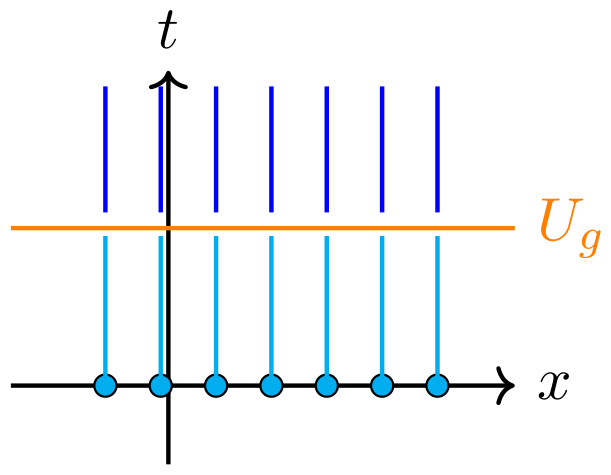
\includegraphics[width=0.24\linewidth]{figures/figure-5.png}
  \caption{带拓扑缺陷的一维格点。（原文 Figure~5，PDF 第 21 页）}
  \label{Fig:lattice-TDN}
\end{figure}

    拓扑缺陷算符必须遵从群的表示，这可以写成
    \be U_{g} U_{h} = U_{gh}. \ee
    该运算可以理解为拓扑缺陷 $U_g$ 与 $U_h$ 融合为 $U_{gh}$，如下式所示：
    \be
        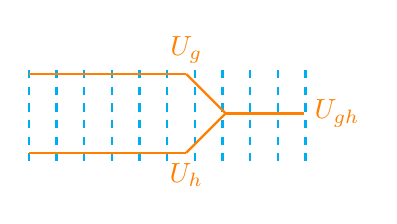
\begin{tikzpicture}
        \draw[color = cyan, thick,dashed] (-1,0.05)--(-1,-1.2)
        [shift = {(10pt,0)}] (-1,0.05)--(-1,-1.2)
        [shift = {(10pt,0)}] (-1,0.05)--(-1,-1.2)
        [shift = {(10pt,0)}] (-1,0.05)--(-1,-1.2)
        [shift = {(10pt,0)}] (-1,0.05)--(-1,-1.2)
        [shift = {(10pt,0)}] (-1,0.05)--(-1,-1.2)
        [shift = {(10pt,0)}] (-1,0.05)--(-1,-1.2)
        [shift = {(10pt,0)}] (-1,0.05)--(-1,-1.2)
        [shift = {(10pt,0)}] (-1,0.05)--(-1,-1.2)
        [shift = {(10pt,0)}] (-1,0.05)--(-1,-1.2)
        [shift = {(10pt,0)}] (-1,0.05)--(-1,-1.2);

        \draw[orange, thick] (-1,0)--(1,0) node[anchor = south]{$U_g$};
        \draw[orange, thick] (-1,-1)--(1,-1) node[anchor = north]{$U_h$};
        \draw[orange, thick] (1,0)--(1.5,-0.5);
        \draw[orange, thick] (1.5,-0.5)--(2.5,-0.5) node[anchor = west]{$U_{gh}$};
        \draw[orange, thick] (1,-1)--(1.5,-0.5);


        \end{tikzpicture}
    \ee
    式中蓝色虚线表示各格点上状态的时间演化。需要注意，由缺陷实现的群作用应当是有向的；反方向对应于逆算符 $U_{g^{-1}}$。例如，依次作用缺陷算符 $U_g$、$U_{g^{-1}}$、$U_g$，其结果应与单独作用一次 $U_g$ 相同：
    \be
        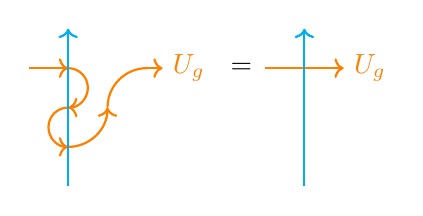
\begin{tikzpicture}
        \draw[orange , thick , ->] (-1,1)--(-0.5,1) ; 
        \draw[orange , thick,->] (0.5,1)--(0.7,1) node[anchor = west]{$U_g$}; 
        \draw[orange , thick,->] (2,1)--(3,1) node[anchor = west]{$U_g$}; 
        \draw[orange,thick,->] (-0.5,1) arc (90:-90:0.25);
        \draw[orange,thick,->] (-0.5,0.5) arc (90:270:0.25);
        \draw[orange,thick,->] (-0.5,0) arc (-90:0:0.5);
        \draw[orange,thick] (0,0.5) arc (180:90:0.5);
        \draw[cyan,thick,->] (-0.5,-0.5) -- (-0.5,1.5);
        \draw[cyan,thick,->] (2.5,-0.5) -- (2.5,1.5);

        \node[] at (1.7,1) {$=$};
        \end{tikzpicture}
    \ee

    此外，$U_{g^{-1}}$ 与 $U_g$ 的逆关系可以表示为：
    \be\label{Prop:bubble}
        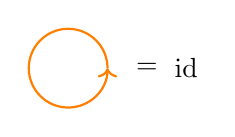
\begin{tikzpicture}
        \draw[thick, orange ,->] (-0.5,0) arc (0:360:0.5);
        \node[] at (0,0) {$=$};%{$\propto$};
        \node[] at (0.5,0) {id};
        \end{tikzpicture}
    \ee
    这样的“气泡”总可以加入 TDN 中，而实际上不改变尊重该对称性的系统。

    \item \label{para:flatconn}\textbf{平坦联络}。在格点规范理论、或等价地在 Čech 上同调的语境中，我们用 $i$、$j$、$k$ 等指标给格点贴标签。1-形式规范联络（记为 $A$）负责把群元素赋给连接格点的连线（link）。也就是说，若格点 $i$ 与格点 $j$ 之间有一条连线，则 $A_{ij} \in G$，其中 $G$ 是我们所研究的群。然而这一赋值并非任意，它必须服从特定条件，例如
    \be A_{ij}\cdot A_{jk} \cdot A_{ki} = {\rm id} = A_{ij} \cdot A_{ji} \ . \label{Eq:Flatcondition}\ee
% ==== 原文 PDF 第 22 页 ====
    这一条件刻画了所谓平坦联络。事实上，在连续极限下，式~(\ref{Eq:Flatcondition}) 可以解释为线积分
    \be  \oint A = 0. \ee
    此情形下的规范变换为
    \be\label{gaugetransf1} A_{ij} \mapsto A_{ij}'=g_i^{-1} A_{ij} g_j,  \ee
    从而
    \be \int_{i\to j} A = A_{ii_1}\cdot A_{i_1 i_2}\dots A_{i_n j} \mapsto g_i^{-1} \cdot (\int_{i\to j} A) \cdot g_j. \ee
    若取闭合回路作积分，我们看到威尔逊圈是规范不变的，正如所预期。

    \item \textbf{分类空间}。这是一个更为抽象的概念；本节旨在提供直观理解，而非严格证明。主要想法是构造一个空间 $BG$，使得任何主丛 $P\to M$ 都可以通过一个映射 $\phi : M\to BG$ 拉回得到，如图~\ref{Fig:ClassSpace} 所示。在此语境中，$EG\to BG$ 表示“万有 $G$-丛”，它可被拉回而给出任意 $G$-丛。这看起来或许复杂，但若回想我们此前对平坦联络的理解，就能看出真正重要的是把群元素赋给连接各格点的连线的信息；格点本身的细节对我们的目的而言变得不那么重要。更详细的描述请参见例~\ref{Eg:GT}。指定一个规范场构型本质上等价于定义各路径的和乐，而这又对应于从时空到分类空间 $BG$ 的映射。
    \begin{figure}[htbp]
        \centering
            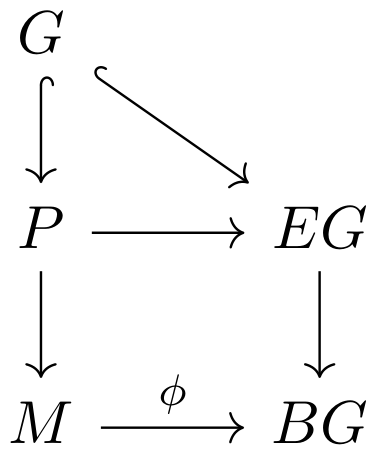
\includegraphics[width=0.15\linewidth]{figures/figure-6.png}
        \caption{分类空间与万有丛。（原文 Figure~6，PDF 第 22 页）}
        \label{Fig:ClassSpace}
    \end{figure}

\begin{definition}
群 $G$ 的分类空间（记作 $BG$）是一个拓扑空间，它具有性质 $\pi_1(BG) \cong G$，而对所有不等于 1 的 $n$ 都有 $\pi_n(BG) = 0$。
\end{definition}

% ==== 原文 PDF 第 23 页 ====
映射 $\phi: M\to BG$ 把时空流形 $M$ 中的点映到分类空间 $BG$ 中的那个单点，并把 $M$ 中的路径映到群元素，如前所述。必须认识到，同伦等价的映射 $\phi$ 给出时空流形 $M$ 上等价的 $G$-丛。从规范场联络的角度看，这种等价对应于式~(\ref{gaugetransf1}) 中规范等价的规范场构型 $A$ 与 $A'$。这样，数学中同伦的概念就翻译成了物理中规范变换的概念。

\end{enumerate}

把前述三种视角从 0-形式对称性推广到高形式对称性是一个直接的过程。下面给出概览：

\begin{enumerate}
    \item \textbf{拓扑缺陷网络}（几何直观）。在这一视角下，拓扑缺陷是嵌入 $d$ 维时空中的 $(d-p-1)$ 维对象。这些对象能够沿更低维的流形彼此结合或相互作用。缺陷网络为理解高 $p$-形式对称性在给定物理系统中如何作用提供了一份独特而精确的指南；它勾勒出该对称性作用于系统的规则与模式。这一做法给我们以几何直观，因为所有算符都关联于时空流形内的子流形。

    \item \textbf{平坦联络}（物理计算）。在此语境中，联络取 $(p+1)$-形式，它建立群元素与时空流形中 $(p+1)$-单纯形之间的赋值。例如，1-形式对称性对应 2-形式规范场。在格点框架中，这些规范场把群元素（对阿贝尔群 $G$ 记为 $g_{ijk}$）赋给时空流形三角剖分中的三角形，后者记为 $\langle ijk\rangle$。这些联络同样受平坦联络条件的约束，这意味着与一个四面体边界上全部四个三角形相联系的群元素之和等于 $G$ 中的平凡元素。这一做法的优点是：我们可以容易地用规范场写出作用量与规范变换规则，因而很适合物理计算。
    
    \item \textbf{分类空间}（拓扑分类）。我们现在有分类映射 $\phi: M^d\to B^{p+1}G$，其中 $B^{p+1}G=K(G,p+1)$ 是 Eilenberg–MacLane 空间，其定义为 $\pi_{p+1}(B^{p+1}G) \cong G$，而所有其他同伦群平凡。
% ==== 原文 PDF 第 24 页 ====
从时空流形 $M^d$ 到 Eilenberg–MacLane 空间的映射，等价于把 $G$ 中的群元素赋给时空流形三角剖分的 $(p+1)$ 维单纯形。这些赋值自动满足平坦联络条件。这一做法把物理问题转化为同伦问题，因而适用于分类，例如理解高形式对称性中的反常。
    
    \end{enumerate}

% ============================================================
% 片段：s03a  对应原文 section2.tex 第 647--877 行；PDF 第 24--32 页
% 内容：§3 Anomalies and SPT（3.1 及其三个小节）
% 译者：t-s03a   审校状态：初稿
% ============================================================

% ==== 原文 PDF 第 24 页 ====
\section{反常与 SPT}\label{sec:anomalies}

\begin{keytakeaways}
  \begin{itemize}[leftmargin=1.4em,itemsep=2pt,topsep=2pt]
    \item \textbf{物理图像}：'t Hooft 反常用整体对称性与规范不变性的冲突来刻画——把整体对称性推广为背景规范场后，配分函数在局域规范变换下不再不变，而是多出一个相位因子。该相位无法靠局域抵消项消去，只能由高一维的 SPT 体通过反常流入（anomaly inflow）吸收。
    \item \textbf{数学工具}：群上同调。0+1 维反常与 1+1 维 SPT 由 $H^2_{\rm grp}(G,U(1))$ 分类；1+1 维反常与 2+1 维 SPT 由 $H^3_{\rm grp}(G,U(1))$ 分类。上闭链条件正是结合律（0+1 维）与五边形方程（1+1 维）的体现，上边缘则对应可自由重定义的局域抵消项。
    \item \textbf{关键结论}：SPT 相的边界必然带有非平凡 't Hooft 反常，因此非平凡 SPT 相不可能拥有既保持能隙、又保持对称性、且不含拓扑序的边界。
    \item \textbf{关键例子}：Haldane 链是受 $SO(3)$（或其子群 $\mathbb{Z}_2\times\mathbb{Z}_2$）保护的 SPT 相，其边界自旋-$\frac{1}{2}$ 构成 $SO(3)$ 的投影表示，对应第二 Stiefel--Whitney 类 $\frac{1}{2}w_2$；AKLT 模型的四重简并基态给出该边界自由度的显式实现。
  \end{itemize}
\end{keytakeaways}

本节将在前文关于对称性的综合视角下回顾 't Hooft 反常（'t Hooft anomaly），并说明其与 SPT 相（symmetry-protected topological phase，对称保护拓扑相）的联系~\cite{chen2011two,chen2012chiral,elsenayak2014,kapustin2014anomalous,kapustin2014anomalies,kapustin2014symmetry,thorngren2015higher,wang2015bosonic,chenjie2016,bultinck2018global,wan2018higher,wang2018symmetric,TI4,TI5}。第~\ref{sec:anomaly-SPT}~节的讨论集中于 't Hooft 反常与高一维 SPT 相之间的关系；为简单起见，重点放在 1 维与 2 维的反常上，并以凝聚态物理中一个众所周知的例子来说明：Haldane 链边界上带反常的自旋-$\frac{1}{2}$。第~\ref{sec:gen-SPT}~节面向进阶读者，深入探讨 't Hooft 反常与 SPT 相的一般分类，涉及高维系统、高形式对称性、费米子系统与配边等较复杂的主题。该部分虽有价值，但超出入门水平，初学者可以先行跳过、日后再读。

\subsection{SPT 边界上的 't Hooft 反常}\label{sec:anomaly-SPT}

对于由作用量 $S[\phi]$ 描述、含物质场 $\phi$ 的理论，首先必须明确\emph{整体}对称性的含义：它可以是离散的，未必由无穷小变换生成。我们先指定物质场的对称变换，对每个 $g\in G$ 记 $\phi\mapsto \phi^g$，其中 $G$ 表示对称群。物质场 $\phi$ 的量子系统要具有整体对称群 $G$，要求在这些变换下满足
\begin{align}\label{gaugetransf}
S[\phi] = S[\phi^g] \quad \text{且} \quad \mathcal{D}\phi = \mathcal{D}\phi^g, \quad \forall g\in G.
\end{align}
此时称由配分函数 $Z = \int \mathcal{D}\phi \exp(iS[\phi])$ 定义的理论具有由群 $G$ 刻画的整体对称性。

下面把背景规范场（background gauge field）$A$ 耦合到理论中，考察其推论。这里所谓背景规范场，是指只对物质场 $\phi$ 作积分，而把规范场 $A$ 固定：
\be Z[A] = \int\mathcal{D}\phi e^{iS[A,\phi]} \ . \ee

% ==== 原文 PDF 第 25 页 ====
当 $Z[A]$ 不等于 $Z[A^g]$、即 $Z[A]$ 在\emph{局域}规范变换下不再保持不变时，就出现 't Hooft 反常。的确，由于 $Z[A]$ 不具备规范不变性，对规范场 $A$ 作积分（integrate out）便成为问题：我们实际上是在规范场 $A$ 的规范轨道上积分。为处理这一点，引入 $Z[A]$ 中对 $A$ 作规范化（gauging）存在障碍这一概念，该障碍由下式描述：
\be
Z[A^g] = Z[A]\cdot Z_{\text{anomaly}} [A,g],
\ee
其中 $g$ 表示\emph{局域}规范变换，而不是式~(\ref{gaugetransf}) 中的整体变换。相位因子 $Z_{\text{anomaly}}[A,g] \in U(1)$ 刻画该理论的 't Hooft 反常。

\begin{yizhu}
式 (3.3) 中的 $Z_{\text{anomaly}}[A,g]$ 不是 $A$ 与 $g$ 的任意相位：把两次局域变换复合为一次时，它必须满足上闭链型的相容条件，因此其取值是离散的，构成由 $H^{d+1}(BG,U(1))$ 刻画的离散数据（即反常系数）。这正解释了 't Hooft 反常为何不能靠加局域抵消项消除：抵消项只能改变上边缘，改变不了上同调类。另需注意 $Z[A]$ 只对物质场积分、$A$ 保持固定，故 $Z_{\text{anomaly}}$ 一般不是 $A$ 的局域泛函。
\end{yizhu}

从第~\ref{sec:three}~节所讨论的关于物理系统对称性的三个视角来看，'t Hooft 反常揭示如下含义：
\begin{enumerate}
\item \textbf{拓扑缺陷网络（TDN）视角}。在此视角下，$G$-对称性缺陷失去拓扑性质。特别地，当通过时空中拓扑缺陷的重新连接这类局域操作改变网络的拓扑时，会额外出现相位因子；这些额外相位因子正是对称性反常的标志。
\item \textbf{平坦联络视角}。这里，TDN 的局域变换可以翻译为规范场的规范变换。于是，配分函数在 TDN 局域改变下不再保持不变这一事实，就翻译为等价的规范场联络给出不同的配分函数，换言之 $Z[A^g]\neq Z[A]$。
\item \textbf{分类空间视角}。在此视角下，规范变换与映射 $\phi: M^d\rightarrow B^{p+1}G$ 的同伦性质相关。因此，带反常的配分函数 $Z: [M^d, B^{p+1}G]\rightarrow \mathbb{C}$ 并不是同伦类 $[\phi]$ 上的良定义函数（$[\phi]$ 表示 $M^d$ 到 $B^{p+1}G$ 的映射同伦类），而依赖于同伦类 $[\phi]$ 中映射 $\phi$ 的具体选取。
\end{enumerate}

\subsubsection{0+1 维 't Hooft 反常与 1+1 维 SPT}
\label{subsubsec:0+1D}

考虑一个具有 0-形式整体对称性 $G$ 的 0+1 维系统。在这个一维时空中，群元 $g\in G$ 的作用由插入一个作用在系统希尔伯特空间上的点算符 $U_g$ 来体现。由于整体对称性的性质，$U_g$ 插入的精确位置没有意义。再者，$U_h$ 与 $U_g$ 的相继作用完全等价于单个算符 $U_{gh}$ 的作用。这一等价关系可以理解为一次改变 TDN 拓扑的局域操作。
% ==== 原文 PDF 第 26 页 ====
数学上，这一关系写成
\be
U_gU_h=U_{gh}.
\ee
该式表明，$U_g$ 的作用在 0+1 维系统的希尔伯特空间上构成群 $G$ 的线性表示。

\begin{yizhu}[原文疑误]
源码与 PDF 中有三处小疵，均照原文保留：其一，第 25--26 页（印刷页码）出现“the topology of the topology of TDN”的重复，译文按本义只作一次拓扑理解；其二，第 28 页（印刷页码）对式 (3.11) 的引用写作 Eq.~(ref\{eq:tri\})，缺一个反斜杠，PDF 中实际排成 (refeq:tri)；其三，第 29 页（印刷页码）“This is believed to leads to a gapless state”中 leads 应为 lead。
\end{yizhu}

反之，若放松 TDN 在局域操作下保持不变这一假设，则引入修改后的方程
\be\label{UgUhUgh}
U_gU_h = \omega(g,h) U_{gh}.
\ee
这里 $\omega: G\times G \rightarrow U(1)$ 引入一个额外的相位因子。必须注意，这个相位因子 $\omega$ 并非任意：希尔伯特空间上的 $G$-作用必须满足结合律，由此得到要求
\be\ba
&\quad (U_g\cdot U_h)\cdot U_k = U_g\cdot (U_h\cdot U_k)\cr
&\Rightarrow \omega(g,h)\omega(gh,k) U_{ghk} = \omega(g,hk)\omega(h,k) U_{ghk}\cr
&\Rightarrow\omega(g,h)\omega(gh,k)  = \omega(g,hk)\omega(h,k). \cr
\ea\ee
这一相容性条件可以解释为群上同调中的 2-上闭链条件，确切地说：
\be (\dd_2 \omega) (g,h,k) := \frac{\omega(h,k)\omega(g,hk)}{\omega(gh,k)\omega(g,h)} = 1. \ee
关于群上同调的更完整讨论，参见附录~\ref{App:GrpChmlg}。

\begin{yizhu}
式 (3.7) 与 (3.10) 采用的是乘法记号的群上同调：$\dd_2$ 表达式中分子与分母的次序对应一种归一化约定；若把群运算写成加法（$G$ 阿贝尔、相位写成 $\mathrm{e}^{i\alpha}$），它等价于 $\dd\alpha=\alpha(h,k)-\alpha(g,hk)+\alpha(gh,k)-\alpha(g,h)$。推导 (3.6) 时隐含假设了 $U_{ghk}$ 可逆、可从两边消去；这对 $U(1)$ 相位因子自动成立，但对一般算符需另作说明。此外 (3.7) 写 $\dd_2$、(3.19) 写 $\dd$，二者分别是 2-上边缘与 3-上边缘算子，不要与 (3.9) 中的 $\dd_1$ 混为同一符号。
\end{yizhu}

通过引入相位因子 $\lambda(g)$，可以修改作用在系统希尔伯特空间上的对称性作用 $U_g$ 的定义：
\be
U_g \mapsto U_g' = \lambda(g) U_g.
\ee
这一修改的效果是把 2-上闭链 $\omega$ 变为新函数
\be
\omega(g,h)\mapsto \omega'(g,h )= \omega(g,h)\lambda(h)   \lambda(g)\lambda(gh)^{-1} =(\omega\cdot \dd_1\lambda)(g,h) \ . 
\ee
注意 ${\text{im}(\dd_1)}$ 中的元素可以解释为一个整体 $U(1)$ 相位，它只是描述量子系统时所作的一种选择，没有物理意义，因此在我们的描述中应当被商掉。于是相位因子 $\omega$ 是群 $G$ 的第二上同调群的元素，定义为：
\be H^2_{\rm grp}(G,U(1))  =  \frac{{\rm ker}(\dd_2)} {{\rm im}(\dd_1)} \ . \ee
指定一个相位因子 $\omega \in H^2_{\text{grp}}(G, U(1))$，等价于定义群 $G$ 的一个投影表示（projective representation）。

% ==== 原文 PDF 第 27 页 ====
以上分析揭示了 0+1 维量子场论中 't Hooft 反常与上同调群 $H^2_{\rm grp}(G,U(1))$ 之间的有趣联系。该上同调群是分类群 $G$ 的投影表示的关键工具。有趣的是，上同调群 $H^2_{\rm grp}(G,U(1))$ 在物理中还有另一项关键作用：它是 1+1 维 SPT 态的分类方案~\cite{SPT1D1,SPT1D2,SPT1D3,SPT1D4}。SPT 相是由对称性提供非平凡保护的有能隙物态。值得注意的是，以 $\omega \in H^2_{\rm grp}(G,U(1))$ 刻画 't Hooft 反常的 0+1 维量子场论，与同样带有该 $\omega$ 的 1+1 维 $G$-SPT 相之间存在直接对应。这一对应表明，带 't Hooft 反常的 0+1 维量子场论可以看作 1+1 维 SPT 相的边界理论。因此，非平凡 SPT 相不可能拥有既保持能隙、又保持对称性且不含拓扑序的边界，因为这样的边界必然带有非平凡 't Hooft 反常。

\begin{center}
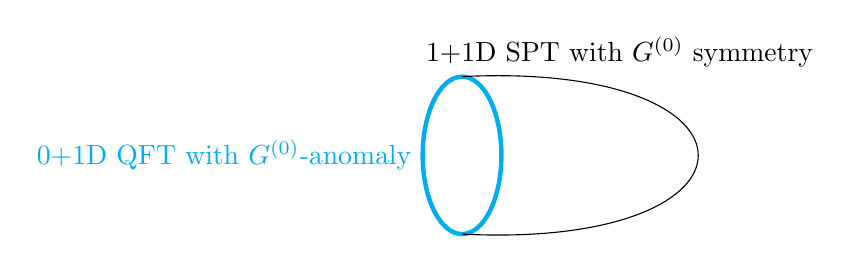
\begin{tikzpicture}
    \draw[ultra thick, cyan] (0,0) ellipse (0.5 and 1) (-0.5,0)node[left]{0+1D QFT with $G^{(0)}$-anomaly} ;
    \draw (0,1) .. controls (4,1.2) and (4,-1.2) .. (0,-1) (2,1)node[above]{1+1D SPT with $G^{(0)}$ symmetry};
\end{tikzpicture}
\end{center}

为理解 0+1 维 't Hooft 反常与 1+1 维 SPT 相之间的关系，可以从显式构造 1+1 维 SPT 系统在格点上的配分函数入手。定义该配分函数的步骤如下：
\begin{enumerate}
    \item 为 1+1 维闭时空流形 $M$ 选取一个三角剖分。
    \item 用 $G$ 中的群元标记三角剖分的每条边，并要求在每个三角形内满足平坦联络条件，即
    \be\label{eq:tri}
        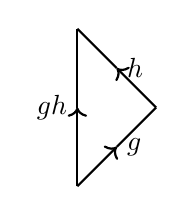
\begin{tikzpicture}
            \draw[thick,->] (0,0)--(0,1);
            \draw[thick] (0,1)--(0,2) (0,1)node[left]{$gh$};
            \draw[thick,->] (0,0)--(0.5,0.5)  node[right]{$g$};
            \draw[thick] (0.5,0.5)--(1,1);
            \draw[thick,->] (1,1)--(0.5,1.5) node[right]{$h$};
            \draw[thick] (0.5,1.5)--(0,2);
        \end{tikzpicture}
    \ee
    这种边标号本质上给出平坦联络 $A: M \to BG$ 的离散表示：$M$ 中每条不同路径对应一个群元，它由沿各条链路的群元相乘得到。
    \item 每个基本三角形（一般维数下为单纯形）为配分函数贡献一个元素 $\omega_2(g, h)^{\pm 1} \in U(1)$，符号 $\pm$ 随三角形的定向而变。
    % ==== 原文 PDF 第 28 页 ====
    函数 $\omega_2$ 可以解释为映射 $ BG \to B^2 U(1) $，由于同构
    \be [BG, B^2U(1)]\cong H^2(BG,U(1))\cong H_\mathrm{grp}^2(G,U(1)).  \ee
    它落在第二上同调群 $H^2(BG, U(1))$ 中。
    \item 对任意平坦联络构型 $A$，配分函数表示为 $\omega_2$ 在全部三角形上的乘积，并计入各三角形的定向~\cite{chen2013symmetry}：
    \be Z[A] =  \exp{i \int_M L} = \prod_{\Delta} e^{iL(\Delta)} = \prod_{\Delta} \omega_2 (A(\Delta)) = \prod_{\Delta}A^* (\omega_2)(\Delta).
    \ee
\end{enumerate}

\begin{yizhu}
式 (3.11) 的三角形把两条边标为 $g$ 与 $h$、第三条边标为 $gh$，这等价于要求沿这个闭三角形走一圈所得的群元之积为单位元，即联络平坦。注意其中隐含了定向约定：箭头指明行走方向，逆着箭头走时该边的标号取逆元 $g^{-1}$，而作者并未写出这一点；但判断 $\omega_2(g,h)$ 取 $+1$ 还是 $-1$ 恰恰需要它（这正是第 3 步中符号 $\pm$ 的来源）。在更一般维数下，同一条件表现为 $(p+1)$-单纯形各面上标号的相容性。
\end{yizhu}

这一构造给出了定义 1+1 维 SPT 系统配分函数的普适方式：它以三角剖分中的边标号为基础，并计入各个三角形的贡献，从而在配分函数与上同调类 $ \omega_2 \in H^2_\mathrm{grp}(G,U(1))$ 之间建立起直接对应。

当考察开的 1+1 维时空流形时，0+1 维 't Hooft 反常与 1+1 维 SPT 相之间的复杂关系变得格外透明。具体地，考虑边界附近的一个三角形，如式~(ref{eq:tri}) 所示。去掉这样一个三角形可以理解为一次边界局域操作，它使边界边的数目改变一条。在此语境下，边上的每个群元标号对应对偶 TDN 表示中算符 $U_g$ 的插入。当边界附近的一个三角形被去掉时，边界上的对称性作用从 $U_{gh}$ 变为 $U_gU_h$。这一改变导致相位出现偏差，即式~(\ref{UgUhUgh}) 中的 $\omega(g,h)$，它正是 't Hooft 反常的标志。值得注意的是，该相位因子恰好抵消被去掉的三角形对 1+1 维体 SPT 配分函数的贡献。这揭示了一般的反常流入（anomaly inflow）机制：包含边界与体的组合系统仍保持物理自洽性与规范不变性。这一认识确认，非平凡 SPT 态不可能具有平凡有能隙的对称边界，因为边界理论表现出非平凡 't Hooft 反常。

\subsubsection{例：Haldane 链边界上的反常自旋-$1/2$}

为深入考察体--边对应这一现象，来看一个奠基性的例子：1+1 维 Haldane 链~\cite{haldane1983nonlinear,haldane1983continuum} 与其带反常的 0+1 维自旋-$\frac{1}{2}$ 边界之间的关系。该例说明 't Hooft 反常如何与高一维的 SPT 相联系。

Haldane 链是 1+1 维自旋-$s$ 链，其海森堡相互作用为
\be\label{eq:Haldane}  H = \sum_{\expval{ij}} \vb{S}_i\cdot \vb{S}_j. \ee
% ==== 原文 PDF 第 29 页 ====
在低能极限下，Haldane 证明该模型可被一个连续量子场论有效描述，其配分函数为
\be\ba 
Z &= \int \mc{D} \vb{n} \exp(i\int_{M^2} (\ptl_\mu \vb{n} )^2 \dd^2 x + i  \theta \mathcal{N}[\vb{n}]  ),
\ea\ee
其中 $\mathcal{N}$ 表示场 $\mathbf{n}: M^2 \rightarrow S^2$ 的绕数（即映射度）。第二项中的参数 $\theta=2\pi s$ 与链的自旋 $s$ 有关。

对整数自旋 $s$，由于 $\mathcal{N}$ 取整数，第二项 $e^{i\theta \mathcal N}$ 在闭流形 $M^2$ 上积分后化为 $e^{2\pi i} = 1$。因此，若只保留第一项非线性 sigma 模型，理论在重整化群流下将流向有能隙的对称无序态。相反，对半奇数自旋 $s$，该项依 $\mathcal{N}$ 的奇偶取 $\pm 1$，从而在路径积分中导致相消干涉，据信这给出无能隙态。对反铁磁 1+1 维海森堡模型，$s$ 的这种有能隙/无能隙依赖关系称为 Haldane 猜想~\cite{haldane1983nonlinear,haldane1983continuum}。

自旋-1 Haldane 链的非平凡边缘态可以通过开 1+1 维链的配分函数来理解。沿 0+1 维边界，$\theta$ 项变为自旋-$1/2$ 系统的 Wess--Zumino--Witten 模型~\cite{ng1994edge}。1+1 维体中的自旋-1 自由度（d.o.f.）与边界上的自旋-$1/2$ 自由度之间的关键差别在于其对称群：自旋-1 自由度构成自旋转动对称群 $SO(3)$ 的线性表示，而自旋-$1/2$ 自由度构成 $SU(2)$ 的线性表示、同时构成 $SO(3)$ 的投影表示。由此可以看出，Haldane 链是受 $SO(3)$ 自旋转动对称性保护的 SPT 态~\cite{gu2009tensor}。其边界对应一个自旋-$1/2$ 系统，具有分数化荷，无法在保持对称性的前提下被打开能隙。因此，0+1 维自旋-$1/2$ 的 $SO(3)$ 't Hooft 反常被受同一 $SO(3)$ 群保护的 1+1 维 SPT 体抵消。边界 't Hooft 反常与体内 SPT 相之间的这一有趣关系，阐明了对称性与拓扑在 Haldane 链独特性质中的作用。

要更直接地看出自旋-1 Haldane 链的边界是具有 $SO(3)$ 投影表示的自旋-$1/2$，可以借助 AKLT 模型~\cite{affleck2004rigorous}。该模型可图示如下：
\begin{center}
    
\begin{tikzpicture}
        \filldraw[cyan] (0,0) circle (0.15);
        \filldraw[shift = {(1,0)},cyan] (0,0) circle (0.15);
        \filldraw[shift = {(2,0)},cyan] (0,0) circle (0.15);
        \filldraw[shift = {(3,0)},cyan] (0,0) circle (0.15);
        \filldraw[shift = {(4,0)},cyan] (0,0) circle (0.15);
        \filldraw[shift = {(5,0)},cyan] (0,0) circle (0.15);
        \filldraw[shift = {(6,0)},cyan] (0,0) circle (0.15);
        \filldraw[shift = {(7,0)},cyan] (0,0) circle (0.15);
        \draw[thick] (0.5,0) ellipse (0.8 and 0.4 );
        \draw[shift = {(2,0)}, thick] (0.5,0) ellipse (0.8 and 0.4 );
        \draw[shift = {(4,0)}, thick] (0.5,0) ellipse (0.8 and 0.4 );
        \draw[shift = {(6,0)}, thick] (0.5,0) ellipse (0.8 and 0.4 );
        \draw[thick,blue] (1,0)--(2,0);
        \draw[shift = {(2,0)},thick,blue] (1,0)--(2,0);
        \draw[shift = {(4,0)},thick,blue] (1,0)--(2,0);
        
    \end{tikzpicture}
\end{center}
这里，蓝点代表自旋-$1/2$ 粒子；包围两个自旋-$1/2$ 粒子的椭圆表示投影到每个格点上的自旋-1 三重态；连接两个自旋-$1/2$ 粒子的蓝线表示二者之间的单态。
% ==== 原文 PDF 第 30 页 ====
可以证明，哈密顿量~\cite{affleck2004rigorous}
\be
H_\mathrm{AKLT} = \sum_{\expval{ij}} \left[ \vb{S}_i\cdot \vb{S}_j + \frac{1}{3} (\vb{S}_i\cdot \vb{S}_j)^2 \right]
\ee
的基态恰为上图所示的态。数值计算确认，AKLT 模型与式~(\ref{eq:Haldane}) 中的反铁磁海森堡模型属于同一相，其间没有相变。在闭合的一维空间环上，AKLT 模型的基态唯一；而在开链上，由于链两端存在悬垂的自旋-$1/2$ 粒子，基态为四重简并。因此可以显式看到，自旋-1 Haldane 链的边界是自旋-$1/2$ 系统，其 $SO(3)$ 对称性反常表现为投影表示而非线性表示。

\begin{yizhu}
开链基态是四重简并而非二重，可由边界条件的图像理解：开链两端各留一个悬垂的自旋-$\frac{1}{2}$（每个格点的自旋-1 由两个自旋-$\frac{1}{2}$ 投影得到，链端只余其中一个），每个悬垂自由度给出二重简并，两端相互独立，故简并度为 $2\times 2=4$。这也是 AKLT 模型对 SPT 相的存在性证明：它给出严格可解的基态，说明 Haldane 相与反铁磁海森堡模型同相（Haldane 猜想），而不必依赖数值结果；作者此处只提数值计算，未展开这一论证。
\end{yizhu}

从 SPT 相的角度看，1+1 维 Haldane 相受对称群 $SO(3)$ 或其子群 $\mathbb{Z}_2 \times \mathbb{Z}_2$ 保护。1+1 维 SPT 相与 0+1 维 't Hooft 反常都可以用对称群的投影表示来分类。具体地，可以考察 $SO(3)$ 与 $\mathbb{Z}_2 \times \mathbb{Z}_2$ 以 $U(1)$ 为系数的第二群上同调：
\be  H_\mathrm{grp}^2 (SO(3),U(1)) = H^2_\mathrm{grp} (\mathbb Z_2\times\mathbb Z_2,U(1)) = \bbZ_2. \ee
$H_{\text{grp}}^2 (SO(3),U(1)) = H^2(BSO(3),U(1)) $ 中的非平凡元素是第二 Stiefel--Whitney 类 $\frac{1}{2}w_2$。因此，1+1 维 $SO(3)$-SPT 的作用量为
\be
S=\frac{1}{2}\int \dd^2 x\ w_2.
\ee

\begin{yizhu}
式 (3.17)、(3.18) 把 $\frac{1}{2}w_2$ 当作 $H^2(BSO(3),U(1))=\mathbb{Z}_2$ 的非平凡元素，有两件事需要留意。其一，$w_2$ 本是取值于 $\mathbb{Z}_2$ 的第二 Stiefel--Whitney 类，它在 $H^2(\,\cdot\,,U(1))$ 中的像由 $\mathbb{Z}_2\subset U(1)$ 给出；写 $\frac{1}{2}w_2$ 时应把它理解为 $\theta=\pi$ 的拓扑项 $S=\frac{\theta}{2\pi}\int w_2$，于是 $S$ 只在模 $2\pi$ 的意义下确定，$\mathrm{e}^{iS}$ 只取 $\pm 1$。其二，若把 $w_2$ 取为整系数上链的具体代表，则改变代表只让 $S$ 改变 $2\pi$ 的整数倍，这正是该反常与 SPT 作用量良定义所要求的。
\end{yizhu}

此外，边界上出现自旋-$\frac{1}{2}$，也恰好对应 $SO(3)$ 或 $\mathbb{Z}_2 \times \mathbb{Z}_2$ 的非平凡投影表示；其 't Hooft 反常同样由第二 Stiefel--Whitney 类刻画。

这个例子清楚地展示了体--边对应（bulk-boundary correspondence）：位于边界上、带 't Hooft 反常的量子场论，恰好对应相应 SPT 态的边界。

\subsubsection{例：1+1 维反常与 2+1 维 SPT}

现在把时空维数提高一维：1+1 维中 $G$ 联络的局域操作对应二维 Pachner 移动，该移动引入一个依赖三个群元的相位因子 $\omega_3$：
% ==== 原文 PDF 第 31 页 ====
\begin{center}
    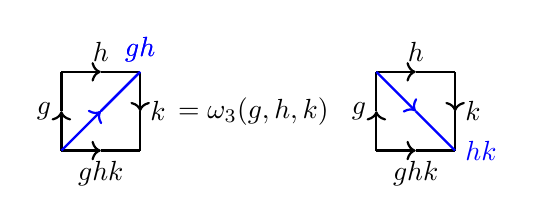
\begin{tikzpicture}
        \draw[thick , ->] (0,0) -- (0.5,0) node[below] {$ghk$};
        \draw[shift={(4,0)}, thick , ->] (0,0) -- (0.5,0) node[below] {$ghk$};
        \draw[thick ] (0.5,0) -- (1,0);
        \draw[shift={(4,0)}, ,thick ] (0.5,0) -- (1,0);
        \draw[thick,->] (0,0)--(0,0.5) node[left]{$g$};
        \draw[shift={(4,0)},thick,->] (0,0)--(0,0.5) node[left]{$g$};
        \draw[thick ] (0,0.5) -- (0,1);
        \draw[shift={(4,0)},thick ] (0,0.5) -- (0,1);
        \draw[thick, ->] (0,1) -- (0.5,1) node[above] {$h$};
        \draw[shift={(4,0)},thick, ->] (0,1) -- (0.5,1) node[above] {$h$};
        \draw[thick] (0.5,1)--(1,1) ;
        \draw[shift={(4,0)},thick] (0.5,1)--(1,1) ;
        \draw[thick , ->] (1,1)--(1,0.5) node[right]{$k$} node[right]{$\  \ \ = \omega_3(g,h,k)$};
        \draw[shift={(4,0)},thick , ->] (1,1)--(1,0.5) node[right]{$k$};
        \draw[thick] (1,0.5)--(1,0);
        \draw[thick,shift={(4,0)}] (1,0.5)--(1,0);
        
        \draw[thick, ->, blue] (0,0)--(0.5,0.5);
        \draw[thick, blue] (0.5,0.5)--(1,1) node[above]{$gh$};
        \draw[shift={(4,0)},thick,-> ,blue] (0,1)--(0.5,0.5);
        \draw[thick, blue] (0.5,0.5)--(1,1) node[above]{$gh$};
        \draw[shift={(4,0)},thick,blue] (0.5,0.5)--(1,0) node[right]{$hk$} ;
    \end{tikzpicture}.
\end{center}
从 2+1 维 SPT 体的角度看，相位因子 $\omega_3(g,h,k)$ 被赋给平坦联络 $A: M^3 \to BG$ 的一个四面体，即
\begin{center}
    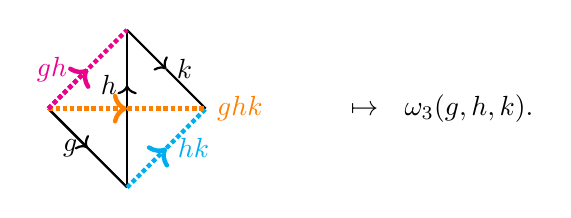
\begin{tikzpicture}
        \draw[->,thick] (0,0)--(0.5,-0.5) node[left]{$g$} ;
        \draw[thick] (0,0)--(1,-1)  ;
        \draw[->,thick] (1,-1)--(1,0.3) node[left]{$h$} ;
        \draw[thick] (1,0)--(1,1) ;
        \draw[->, thick] (1,1)--(1.5,0.5) node[right]{$k$};
        \draw[thick] (1.5,0.5)--(2,0) ;
        \draw[->, ultra thick,cyan,densely dotted] (1,-1)--(1.5,-0.5) node[right]{$hk$} ;
        \draw[ultra thick,cyan, densely dotted] (1.5,-0.5)--(2,0);
        \draw[ultra thick, orange,densely dotted] (0,0)--(2,0) node[right]{$ghk$};
        \draw[ultra thick, orange,densely dotted,->] (0,0)--(1,0);
        \draw[ultra thick, magenta,densely dotted,->] (0,0)--(0.5,0.5) node[left]{$gh \ $};
        \draw[ultra thick, magenta,densely dotted] (0,0)--(1,1);
        \node (a) at (5,0) {$ \mapsto  \ \ \omega_3(g,h,k)$.};
    \end{tikzpicture}
\end{center}
这里，$M^3$ 表示三维时空流形，$BG$ 表示对称群 $G$ 的分类空间（classifying space）。2+1 维 SPT 态的配分函数可表示为时空中各四面体所带相位因子的乘积。把所有这些相位因子的贡献计入后可以看到，原本存在于 1+1 维理论中的 't Hooft 反常被 2+1 维体 SPT 的影响所抵消。这一抵消机制保证了组合系统在对称性与拓扑性质两方面的自洽性。

存在一个支配相位因子 $\omega_3$ 的相容性条件。正如 0+1 维反常中 $\omega_2$ 必须是 2-上闭链，相位因子 $\omega_3$ 也必须满足类似要求，这可由下面的交换图直观表示：
\begin{center}
\begin{tikzcd}
&  & (g(hk))l \arrow[rr, "{\omega_3(g,hk,l)}"] & & g((hk)l) \arrow[rrd, "{\omega_3(h,k,l)}"] &  & \\
((gh)k)l \arrow[rrrd, "{\omega_3(gh,k,l)}"] \arrow[rru, "{\omega_3(g,h,k)}"] &  & & &   &  & g(h(kl)) \\
&  & & (gh)(kl) \arrow[rrru, "{\omega_3(g,h,kl)}"] & &  &         
\end{tikzcd}
\end{center}
上述条件正是 $\omega_3$ 的 3-上闭链条件：
\be
(\dd \omega_3)(g,h,k,l) = \frac{\omega_3(h,k,l) \omega_3(g,hk,l) \omega_3(g,h,k)}{\omega_3(gh,k,l) \omega_3(g,h,kl)} = 1.
\ee
3-上闭链条件作为五边形方程（pentagon equation）的特例，是保证相位因子 $\omega_3$ 在不同四面体之间相容、自洽的基本要求。满足该条件后，相位因子确保 SPT 态良定义且拓扑不变。这一条件对于确立 SPT 相的稳健性与稳定性至关重要，因为它保证系统的物理性质与对称性在各种三角剖分或时空分割下都保持不变。

% ==== 原文 PDF 第 32 页 ====
与 0+1 维反常、1+1 维 SPT 的情形类似，2+1 维 SPT 与 1+1 维反常的上闭链 $\omega_3$ 也存在“规范变换”。该变换来自用局域抵消项（counterterm）重新定义对称性作用。这些抵消项引入一个称为 3-上边缘（3-coboundary）的子群，在反常与 SPT 相的分类中必须把它商掉。因此，分类由第三上同调群 $H_{\mathrm{grp}}^3(G,U(1))$ 决定~\cite{chen2012symmetry,chen2013symmetry}。

% ============================================================
% 片段：s03b  对应原文 section2.tex 第 878--1044 行；PDF 第 32--37 页
% 内容：§3.2 't Hooft 反常与 SPT 的一般分类（3.2.1--3.2.4）
% 译者：t-s03b   审校状态：初稿
% ============================================================

% ==== 原文 PDF 第 32 页（续；本片段自 §3.2 标题起）====
\subsection{'t Hooft 反常与 SPT 的一般分类}\label{sec:gen-SPT}

前面讨论的是具有 0-形式对称性 $G$ 的物理系统的 't Hooft 反常。't Hooft 反常由与规范联络的规范变换、或与群的 TDN 的局域移动相联系的相位因子刻画。我们也说明了，该相位因子对应于高一维 $G$-SPT 配分函数的构造数据。下面将把先前的讨论推广到更高维、高形式对称性、费米子系统与配边分类。这部分内容较为进阶，初学者不妨稍后再重读本节。

\subsubsection{更高维}

这一构造可以直接推广到 $d$ 维时空中的 't Hooft 反常。此时，先对 $d$ 维时空流形作三角剖分；再通过对该剖分的每一条边 $\langle ij \rangle$ 指定一个群元 $g_{ij}$，构造 $G$ 联络的 TDN。在局域重剖分（例如 Pachner 移动）下，这些联络应当彼此等价；但系统会相差一个 $U(1)$ 相位因子 $\omega_{d+1}$。该相位因子刻画系统中 $G$ 对称性的 't Hooft 反常。

此外，$d$ 维剖分的 Pachner 移动可以粘成一个 $(d+1)$ 维单纯形（simplex）。该 $(d+1)$ 维单纯形可理解为高一维 $G$-SPT 配分函数的构造单元。于是，$d$ 维 't Hooft 反常与高一维 $(d+1)$ 维 $G$-SPT 相之间出现直接联系。与 0+1 维中的结合律类似，相容方程由相位因子 $\omega_{d+1}$ 的上闭链条件 $\dd \omega_{d+1}=1$ 刻画。此外，还可对这些相位因子作规范变换，这等价于模去所有 $(d+1)$-上边缘。因此，$d$ 维 't Hooft 反常与 $d+1$ 维 $G$-SPT 相（在低维时）都由 $(d+1)$ 维群上同调分类~\cite{chen2012symmetry,chen2013symmetry}
\be\label{eq:HSPT}
H_{\mathrm{grp}}^{d+1}(G,U(1)) \cong H^{d+1}(BG,U(1)) \cong [BG,B^{d+1}U(1)].
\ee

% ==== 原文 PDF 第 33 页 ====
这里，$H_{\mathrm{grp}}^{d+1}$ 表示群上同调，$H^{d+1}$ 表示拓扑空间通常的（奇异）上同调，而 $[X,Y]$ 表示拓扑空间 $X$ 到 $Y$ 的连续映射的同伦类。

\begin{yizhu}式~\eqref{eq:HSPT} 的两个同构各有实质内容。左端 $H^{d+1}_{\mathrm{grp}}(G,U(1))\cong H^{d+1}(BG,U(1))$ 是群上同调与分类空间上同调之间的标准等同。右端之所以给出上同调，是因为 $B^{d+1}U(1)$ 就是 Eilenberg--MacLane 空间 $K(\mathbb{Z},d+2)$（由 $U(1)=K(\mathbb{Z},1)$ 逐次取分类空间，同伦群次数抬高 $d+1$），故 $[BG,B^{d+1}U(1)]\cong H^{d+2}(BG,\mathbb{Z})\cong H^{d+1}(BG,U(1))$，其中用到 $H^{k}(X,U(1))\cong H^{k+1}(X,\mathbb{Z})$。原文括注“in low dimensions”提示这是低维才成立的结论：维数升高后，群上同调只捕捉 SPT 分类的一部分，漏掉的部分（例如配边群中的自由部分）须由本小节最后讨论的配边分类补足。\end{yizhu}

\subsubsection{高形式对称性}

$d$ 维时空中的 $p$-形式对称性有直接的推广。此时，用阿贝尔群 $G$ 的元素标记三角剖分后时空的 $(p+1)$ 维单纯形。这一标记等价于指定一个映射 $A: M^d \rightarrow B^{p+1}G$，其中 $A$ 可视为 $(p+1)$-形式规范场。当系统作重剖分或 Pachner 移动（代表等价联络之间的规范变换）时，其变化由一个相位因子 $\omega_{d+1}$ 刻画。

与重剖分相联系的相位因子 $\omega_{d+1}$，可理解为构造 $p$-形式 $G$-SPT 配分函数时 $(d+1)$ 维单纯形的相位因子。相容条件给出 $\omega_{d+1}$ 的上闭链条件：$\mathrm{d} \omega_{d+1} = 1$。模去反项重定义（即上边缘）后，$p$-形式 't Hooft 反常与高一维的 $p$-形式 SPT 相都由下式分类：
\be
H^{d+1}(B^{p+1}G,U(1)) \cong [B^{p+1}G,B^{d+1} U(1)].
\ee
该式是式~(\ref{eq:HSPT}) 从 0-形式对称性到 $p$-形式对称性的直接推广~\cite{thorngren2015higher,kapustin2017higher}。

\subsubsection{费米子系统}

$d$ 维时空中 't Hooft 反常与 $(d+1)$ 维时空中 SPT 相之间的关系并不限于玻色子系统，它也延伸到费米子系统。

与玻色子系统相比，费米子系统的对称性结构更为复杂。与玻色子系统不同，费米子系统总具有一个由费米子宇称 $(-1)^F$ 生成、不可破缺的对称性 $\mathbb{Z}_2^f$。一般的费米子对称性 $G_f$ 是费米子宇称与玻色对称性 $G_b$ 的扩张，它可由短正合列（short exact sequence）分类~\cite{wang2020construction}：
\be
1\rightarrow \mathbb Z_2^f \rightarrow G_f \rightarrow G_b \rightarrow 1,
\ee
该扩张由 2-上闭链 $\lambda_2\in H^2_\mathrm{grp}(G_b,\mathbb Z_2^f)$ 支配。

\begin{yizhu}此处“分类”的准确含义是：固定 $G_b$ 后，$G_f$ 作为 $G_b$ 扩张的同构类由群上同调 $H^2_{\mathrm{grp}}(G_b,\mathbb{Z}_2^f)$ 分类，$\lambda_2$ 即该扩张的上闭链代表。物理上 $\mathbb{Z}_2^f$ 必为 $G_f$ 的中心子群（费米子宇称与任何对称性算符对易），故这是中心扩张；$\lambda_2$ 决定玻色对称性在费米子算符上的投影表示（即作用可相差一个费米子宇称相位），其杯积 $\lambda_2\smile n_d$ 并整体进入后文费米子 SPT 相容条件 (3.23) 右端的指数。核对原文时勿把 $\lambda_2$ 当作普通群元。\end{yizhu}

鉴于 't Hooft 反常与 SPT 相之间的关系，要理解费米子系统中的 't Hooft 反常，可以研究高一维的费米子 SPT 相。
% ==== 原文 PDF 第 34 页 ====
与用群上同调分类玻色子系统类似，费米子 SPT 相也存在一种分类，它利用一般群超上同调（general group super-cohomology）作为广义上同调理论~\cite{gu2014symmetry,wang2018towards,Xiong_2018,gaiotto2019symmetry,wang2020construction}。

在这一分类方案中，会用到多层上同调群。例如，玻色 SPT 相可以看作费米子 SPT 相，尽管它在费米子系统中可能变得平凡。因此，最高层对应于玻色层，由 $\omega_{d+1} \in H^{d+1}(G,U(1))$ 表示。此外还存在一个独特的超上同调层，由 $n_d \in H^d(G,\mathbb{Z}_2)$ 表示。这一层本质上涉及把复费米子装饰到时空中 TDN 的相互作用线上。$n_d$ 与 $\omega_{d+1}$ 之间的关系由相容条件约束。在 1+1 维反常或 2+1 维费米子 SPT 相的情形，该条件取一种特殊形式，称为超五边形方程（super-pentagon equation）~\cite{gu2014lattice,gu2015classification}。更一般地，费米子 SPT 相的相容条件表示为~\cite{gu2014symmetry,wang2020construction}
\be
\dd \omega_{d+1} = (-1)^{\lambda_2 \smile n_d + Sq^2(n_d)},
\ee
这里，$Sq^2(n_d) = n_d \smile_{d-2} n_d$ 表示 Steenrod 平方（Steenrod square）的上同调操作~\cite{steenrod1947products}，它与高阶杯积（higher cup product）有关。值得注意的是，该式表明 $\omega_{d+1}$ 不再是上闭链，而只是上链。

第三层通常称为马约拉纳层或 Kitaev 链层，记作 $n_{d-1} \in H^{d-1}_\mathrm{grp}(G_b,\mathbb{Z}_2)$，它起着关键作用。这一层涉及把 Kitaev 链装饰到时空中 TDN 的相互作用面上，从而给支配 $n_d$ 与 $\omega_{d+1}$ 的方程引入额外的扭曲。尽管这一层的障碍函数在低维已为人熟知~\cite{wang2018towards,wang2020construction,kapustin2017fermionic,brumfiel2016pontrjagin,brumfiel2018pontrjagin}，但随着维数升高，它们会变得明显更加复杂。

此外，除了必须满足相容方程，还须计入源于局域反项的上边缘的“规范变换”。值得注意的是，费米子系统呈现出更复杂的规范冗余网络。原则上，只要存在一个反常 SPT 态位于另一个 SPT 态的边界上，该边界 SPT 态就应视为平凡的~\cite{wang2019anomalous}。这是因为存在一个对称的、费米子的局域幺正变换，把该态连接到乘积态。

通过仔细计入这些障碍以及规范冗余（或平凡化），可以系统地构造并分类费米子 SPT 相，以及低一维系统中相应的 't Hooft 反常。

也可以把高形式对称性的研究推广到费米子系统，深入探讨高形式对称性保护的费米子拓扑相的分类。这一探讨与我们对低一维含费米子量子场论中高形式对称性 't Hooft 反常的理解密切相关。
% ==== 原文 PDF 第 35 页 ====
幸运的是，可以借用现有的数学工具，包括超上同调理论与自旋配边理论（spin cobordism），来处理这些费米子系统中的高形式对称性。推广的做法是把 $BG_b$ 换成 $B^{p+1}G_b$，以在所有装饰数据与障碍函数中容纳高形式规范场。重要的是，障碍函数本身保持不变，只是应理解为其自变量现在指由高形式规范场标记的相应单纯形。因此，所有构造与分类方案仍然适用。

\subsubsection{配边分类}

前面讨论了 $d$ 维 't Hooft 反常与 $(d+1)$ 维 SPT 相之间的对应，二者都由对称性的上同调群分类。然而，这一对应虽然在许多情形下是准确的，但在更高维会遇到局限。为处理这一点并提供更完备的框架，下面引入一个更精细的数学工具，即配边（bordism）。

考虑时空流形 $S^2$ 上一个 1+1 维 SPT 态。如前面所讨论，这类理论的配分函数由与剖分中每个三角形相联系的相位因子 $\omega_2$ 相乘得到。为说明这一点，可以先把二维球面 $S^2$ 剖分为单个四面体：
\begin{center}
    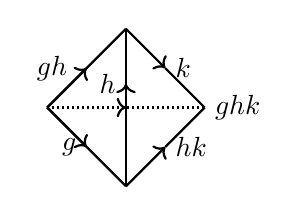
\begin{tikzpicture}
        \draw[->,thick] (0,0)--(0.5,-0.5) node[left]{$g$} ;
        \draw[thick] (0,0)--(1,-1)  ;
        \draw[->,thick] (1,-1)--(1,0.3) node[left]{$h$} ;
        \draw[thick] (1,0)--(1,1) ;
        \draw[->, thick] (1,1)--(1.5,0.5) node[right]{$k$};
        \draw[thick] (1.5,0.5)--(2,0) ;
        \draw[->, thick] (1,-1)--(1.5,-0.5) node[right]{$hk$} ;
        \draw[ thick] (1.5,-0.5)--(2,0);
        \draw[ thick,densely dotted] (0,0)--(2,0) node[right]{$ghk$};
        \draw[ thick,densely dotted,->] (0,0)--(1,0);
        \draw[ thick,->] (0,0)--(0.5,0.5) node[left]{$gh \ $};
        \draw[ thick] (0,0)--(1,1);
        % \node (a) at (5,0) {$ \mapsto  \ \ \omega_3(g,h,k)$.};
    \end{tikzpicture},
\end{center}
此时，配分函数 $Z[S^2]$ 由与该四面体相联系的各相位因子之积给出。数学上可写为：
\be Z[S^2] = \omega(g,h) \omega(gh,k)\omega^{-1} (g,hk) \omega^{-1} (h,k)=1. \ee
最后一步的关键观察是：$\omega_2$ 的上闭链条件得到满足，这保证配分函数等于 1。这意味着 $S^2$ 上的 1+1 维 SPT 态是平凡的。把这一过程递归地应用，可将结果推广到边界配分函数 $Z[\partial M_3]$，它同样等于 1。该结果不仅对 1+1 维成立，对更高维也成立。

\begin{yizhu}[原文疑误]正文称配分函数由每个三角形对应的相位因子 $\omega_2$ 相乘得到，但式 (3.24) 中出现的却是 $\omega$（未写下标 2），二者应指同一个 2-上闭链；译文照抄原文记号，建议核对原稿统一为 $\omega_2$。另外，式 (3.24) 的四个因子与四面体的四个面一一对应：以棱 $g,h,k,hk,gh,ghk$ 标记的四面体中，四个面按定向分别贡献 $\omega(g,h)$、$\omega(gh,k)$、$\omega^{-1}(g,hk)$、$\omega^{-1}(h,k)$，于是上闭链条件恰好使乘积为 1；初学者易漏掉两个 $\omega^{-1}$ 源于相应面的定向相反。\end{yizhu}

现在考虑边界分解 $\partial M_3 = M_2 \sqcup \overline{M_2'}$，可以利用两个取相反定向的面 $M_2$ 与 $\overline{M_2'}$ 把配分函数抵消掉。由此得到方程：
\be\ba  1 = Z[{M_2}]\cdot Z[\overline{M_2'}]  &= Z[M_2]\cdot Z[M_2']^{-1}   \\  
\Rightarrow Z[M_2]  &=  Z[M_2'] \ea\ee
这一观察提示我们引入一个新的等价类。

% ==== 原文 PDF 第 36 页 ====
\begin{definition}
两个 $d$ 维流形 $M_d$ 与 $M_d'$ 若存在一个 $(d+1)$ 维流形 $M_{d+1}$，使得其边界可分解为 $\partial M_{d+1} = M_d \sqcup \overline{M_d'}$，则称二者\textbf{配边等价}（bordism equivalent）。
\end{definition}

属于同一配边类的两个流形，在这一拓扑构造下具有相同的配分函数。此外，我们定义

\begin{definition}
流形的配边环（bordism ring）是三元组 $(\Omega_n^{SO},\sqcup,\times)$。$\Omega_n^{SO}$ 表示 $n$ 维定向流形模去配边等价关系所得的集合。运算 $\sqcup$ 表示不交并，在配边环中充当“加法”运算。运算 $\times$ 对应于笛卡尔积，在配边环中充当“乘法”运算。
\end{definition}

在构造可逆拓扑相（invertible topological phase）时，我们不仅考虑流形，还考虑配有平坦 $G$-联络的流形。此时，理论对每条边指定群 $G$ 中的一个值，并受平坦性条件约束。于是有映射：
\be  A: M_n/{\rm \{ bordism \ equivalence\} } \to BG.   \ee
类似地，可以定义配有平坦 $G$-联络的流形的配边类。相应的配边群记作 $\Omega_n^{SO}(BG)$，它要求联络在体 $M_{n+1}$ 与边界上都相容。

具有对称性 $G$ 的可逆拓扑相的配分函数 $Z$，定义为从配边群到 $U(1)$ 的映射：
\be\label{eq:cobor}  Z: \Omega_n^{SO}(BG)\rightarrow U(1).   \ee
该配分函数使我们能按上述映射的同构类对可逆拓扑序（invertible topological order）分类。该分类由配边群 $\Omega^n_{SO}(BG)$ 表示，它是配边群的 Pontryagin 对偶（Pontryagin dual）。若不计具体的规范群 $G$，并考虑 $BG$ 退化为一个点 $pt$ 的情形，则由于从任何空间到点的映射只有一个，有 $\Omega^n_{SO}(pt) = \Omega^n_{SO}$。

高一维的 't Hooft 反常与 SPT 相由配边描述~\cite{Kapustin:2014tfa,Kapustin:2014dxa,kapustin2014symmetry,freed2014shortrange,brumfiel2016pontrjagin,campbell2017homotopy,brumfiel2018pontrjagin,Wan:2018bns,Wan:2019soo,yonekura2019cobordism,freed2021reflection}。这一新的分类不仅计入 $G$-联络的变化，还允许时空流形本身的拓扑发生变化。它刻画了对称性 $G$ 与底层时空结构之间错综复杂的相互作用，为理解 't Hooft 反常与 SPT 相提供了完备的框架。

% ==== 原文 PDF 第 37 页 ====
另一方面，上同调分类是一种常常更易计算的近似。一般地，存在从群上同调分类到配边分类的群同态；但该群同态既不是单射也不是满射。好消息是，在低维，这个映射是同构，因此两种分类重合。

\begin{example}
一个点的配边群的最简单例子列举如下。
\begin{table}[htbp]
    \centering
    \begin{tabular}{|c|c|c|c|c|c|c|c|c|c|}
    \hline
        $n $ & $0$ & $1$ & $2$ & $3$ & $4$ & $5$ & $6$ & $7$ & $8$ \\
        \hline
        $\Omega_n^{SO}(pt)  $ & $\bbZ$ & $0$ & $0$ & $0$ & $\bbZ$ & $\bbZ_2$ & $0$ & $0$ & $\bbZ^2$ \\
        \hline
        % & $n_{\rm pts+}-n_{\rm pts-}$ &&&& $p_1$ & $w_2 w_3$ &&& $\bbC\bbP^4$, $\bbC\bbP^2\times \bbC\bbP^2$\\
        % \hline
    \end{tabular}
    \caption{一个点的配边分类列表。（原文 Table~1，PDF 第 37 页）}
    \label{tab:bordpts}
\end{table}

在这一例子中，零维由带 $\pm$ 方向的点的数目之差分类（一对 $+$ 方向与 $-$ 方向的点相互抵消）；4 维由第一 Pontryagin 类 $p_1$ 分类；5 维则由 Stiefel--Whitney 类的乘积 $w_2w_3$ 对流形分类。
\end{example}

一般地，$\Omega^n(BG)$ 的分类可能相当复杂。然而存在一种称为 Atiyah--Hirzebruch 谱序列（Atiyah-Hirzebruch spectral sequence）的实用方法，它使我们能利用前面已讨论的低维 $\Omega^n(pt)$ 的知识来计算 $\Omega^n(BG)$。Atiyah--Hirzebruch 谱序列有一个物理解释：把玻色可逆相装饰到群 $G$ 的畴壁上~\cite{chen2014symmetry, wang2021domain}。这一方法为理解并分类对称性及其相关拓扑序提供了有用的工具。

\begin{yizhu}表~\ref{tab:bordpts} 给出的是配边群 $\Omega_n^{SO}(pt)$ 本身（下标群），而 SPT 相的分类实际用的是它的 Pontryagin 对偶 $\Omega^n_{SO}(pt)=\mathrm{Hom}(\Omega_n^{SO}(pt),U(1))$（上标群）：自由部分 $\mathbb{Z}$ 对偶出 $U(1)$（连续的 $\theta$ 角型不变量），挠部分 $\mathbb{Z}_2$ 自对偶出 $\mathbb{Z}_2$（离散不变量），故表中 $n=4,8$ 的自由项与 $n=5$ 的 $\mathbb{Z}_2$ 项在物理上含义不同。表中非零项可由示性类读出：$\Omega_4^{SO}=\mathbb{Z}$ 由第一 Pontryagin 类 $p_1$ 探测，$\Omega_5^{SO}=\mathbb{Z}_2$ 由 $w_2w_3$ 探测，$\Omega_8^{SO}=\mathbb{Z}^2$，而 $n=1,2,3,6,7$ 均为零。要用 $\Omega^n(pt)$ 算出 $\Omega^n(BG)$，靠的是 Atiyah--Hirzebruch 谱序列：其 $E^2$ 页为 $E^2_{p,q}=H_p(BG,\Omega_q^{SO}(pt))$，收敛到 $\Omega_{p+q}^{SO}(BG)$；物理上即把 $q$ 维玻色可逆相装饰到 $G$ 的 $p$ 维畴壁上，各阶微分 $d_r$ 给出装饰的障碍。这也说明，从群上同调分类到配边分类的同态一般既非单射也非满射，仅在低维重合。\end{yizhu}

上述 't Hooft 反常与 SPT 相的配边分类，至少可以在概念上容易地推广到高形式对称性。关键的修改是把 1-形式规范场 $A$ 换成 $(p+1)$-形式规范场；相应地，配边群现在记作 $\Omega_n(B^{p+1}G)$。实践中仍可利用 Atiyah--Hirzebruch 谱序列作为计算这些配边群、理解所涉高形式对称性的有用工具。这一推广使我们能探索广泛的拓扑现象，并对具有高形式对称性的奇异物质相分类。

在费米子系统的语境下，配边等价的概念推广到带有自旋结构（spin structure）或其他切结构（tangential structure）的流形。有趣的是，在低维，配边分类与一般群超上同调分类彼此重合。这一对应使我们能利用 Atiyah--Hirzebruch 谱序列提供的畴壁装饰图像，为计算费米子系统中的 't Hooft 反常提供更便捷的方法。

% ============================================================
% 片段：s04a  对应原文 section2.tex 第 1045--1197 行；PDF 第 38--42 页
% 内容：§4 Applications of Higher-Form Symmetry（§4.1 在弦论中的应用；
%       PDF 第 43 页起为 §4.2，不属本片段）
% 译者：t-s04a   审校状态：初稿
% ============================================================

% ==== 原文 PDF 第 38 页 ====
\section{高形式对称性的应用}\label{sec:applications}

\begin{keytakeaways}
  \begin{itemize}[leftmargin=1.4em,itemsep=2pt,topsep=2pt]
    \item \textbf{物理图像}：几何工程把引力扇区从 QFT 中退耦：超弦/M 理论放在非紧（可能奇异）的 $X$ 上，${\rm vol}(X)\to\infty$ 使 $G_d=G_{11}/{\rm vol}(X)\to0$，只留下奇异点附近的局域模。
    \item \textbf{数学工具}：高形式对称性由 $X$ 的（相对）同调与上同调读出：$C_3/G_4$ 沿 $M_{11-d}$ 的上同调元素展开给出规范场与场强；挠闭链 $[\alpha]$ 给出 $\mathbb{Z}_l$ 的电、磁 $(2-i)$ 和 $(5-i)$-形式对称性。
    \item \textbf{关键结论}：11 维拓扑耦合 $C_3\wedge G_4\wedge G_4$ 约化到 $M_{11-d}$ 上给出 't Hooft 反常多项式；更一般的对称性拓扑场论（SymTFT）作用量可由微分上同调版本给出，并涵盖离散对称性。
    \item \textbf{关键结论}：绕锥 $\Sigma_{i+1}[\alpha]$ 的 M2、M5 膜分别是电、磁对称性的带荷对象；二者由非对易挠通量生成且彼此不局域，绝对理论必须选择极化。
    \item \textbf{关键结论}：5 维 $\mathcal{N}=1$ 超共形场论的库仑分支由 crepant 解奇实现，其 1-形式对称性可由电荷矩阵的 Smith 标准形、链环的同调或场论论证三种方法算出，均得 $\Gamma^{(1)}=\mathbb{Z}_{\text{gcd}(N,k)}$。
  \end{itemize}
\end{keytakeaways}

本节将说明高形式对称性在弦论与凝聚态物理中的一些应用。

考虑到读者来自不同的学术背景，我们鼓励读者阅读与自身当前理解及兴趣相符的主题；尽可聚焦于熟悉的应用，并按需跳过或回头再读其他部分。

\subsection{在弦论中的应用}\label{sec:string}

本节讨论高形式对称性与弦论之间的相互作用，这是近年来颇受关注的研究方向\cite{DelZotto:2015isa,Bergman:2020ifi,Morrison:2020ool,Albertini:2020mdx,Bah:2020uev,Closset:2020scj,DelZotto:2020esg,Apruzzi:2020zot,Cvetic:2020kuw,BenettiGenolini:2020doj,Cordova:2020tij,DelZotto:2020sop,Gukov:2020btk,Heidenreich:2020pkc,Closset:2020afy,Apruzzi:2021phx,Apruzzi:2021vcu,Hosseini:2021ged,Cvetic:2021sxm,Buican:2021xhs,Braun:2021sex,Cvetic:2021maf,Cvetic:2021vsw,Apruzzi:2021mlh,Closset:2021lwy,Apruzzi:2021nmk,DelZotto:2022fnw,Genolini:2022mpi,Benini:2022hzx,Cvetic:2022imb,DelZotto:2022joo,Apruzzi:2022dlm,Hubner:2022kxr,Heckman:2022xgu,Heckman:2022suy,Damia:2022bcd,GarciaEtxebarria:2022vzq,Apruzzi:2022rei,vanBeest:2022fss,Heckman:2022muc,Antinucci:2022vyk,Grimm:2022xmj,Etheredge:2023ler,Amariti:2023hev,DelZotto:2023ahf,Acharya:2023bth,Cvetic:2023plv,Dierigl:2023jdp,Lawrie:2023tdz,Bah:2023ymy,Apruzzi:2023uma,Cvetic:2023pgm}。此处的一般步骤是：先从弦论出发用几何方法构造 QFT，再用几何方法计算高形式对称性。

粗略地说，从弦论构造 QFT 有两种方式，
\begin{enumerate}
    \item AdS/CFT 方案。此时考虑放在 ${\rm AdS}_{d+1} \times  M_{10-d / 9-d}$ 上的超弦/M 理论（对 11 维 M 理论为 (10-d)，对 10 维超弦理论为 (9-d)），它与某个 QFT$_d$ 对偶，后者常被解释为膜对象的世界体积（world-volume）理论。
    \item 几何工程（geometric engineering）方案。此时考虑放在 $\bbR^{d-1,1}\times X$ 上的超弦/M 理论，其中 $X$ 是一个非紧（且可能奇异）的空间，使得引力部分退耦。

    但“退耦”是什么意思？考虑（过度简化的）爱因斯坦–希尔伯特作用量模型，出发点是
    \be \int_{\mb{R}^{d-1,1}\times X}\frac{1}{G_{11}} \sqrt{-g_{11}} R_{11}  \mapsto \int_{\mb{R}^{d-1,1}}\frac{{\rm vol}(X)}{G_{11}} (\sqrt{-g_{d}} R_{d} + \cdots)  \ee
    其中下标 $_{11}/ _{d}$ 表示 11/d 维理论中的量。于是显然，有效 $d$ 维爱因斯坦–希尔伯特耦合常数应满足
    \be G_d = \frac{G_{11}}{{\rm vol}(X)} \ee
    当 $X$ 变为非紧、${\rm vol}(X)\to \infty$ 时，$d$ 维的引力耦合趋于 $0$，这就是“退耦”的图像\footnote{注意，在 vol$(X)\rightarrow\infty$ 的极限下会出现额外的无质量 KK 模。尽管如此，在此类几何工程设定中，人们只考虑原点（奇异点）附近的局域模。}。
\end{enumerate}

\begin{yizhu}
（4.1）与（4.2）是 11 维爱因斯坦–希尔伯特项沿 $X$ 作零模约化的结果：只保留 $X$ 上的常数模，$\int_X \sqrt{-g_{11}} R_{11}$ 便化为 ${\rm vol}(X)$ 乘以 $d$ 维被积函数，故 $1/G_d={\rm vol}(X)/G_{11}$。作者未展开的细节有二。其一，$G_{11}$ 是 11 维牛顿常数，量纲为长度的 9 次方，而 $d$ 维普朗克质量满足 $M_{\rm Pl}^{d-2}=1/G_d$，所以 ${\rm vol}(X)\to\infty$ 等价于 $M_{\rm Pl}\to\infty$，引力确实退耦。其二，该约化默认只保留零模、且 $X$ 的曲率标度远大于 $d$ 维能标；如脚注 8 提示，极限下仍有额外的无质量 KK 模，但几何工程只关心奇异点附近的局域模。建议核对原文第 38 页（4.1）与（4.2）。
\end{yizhu}

下面引入此类理论更具体的设定，并开始考察这些理论中的高形式对称性与 't Hooft 反常多项式。

% ==== 原文 PDF 第 39 页 ====
考虑 11 维 M 理论的红外极限，它正是一个带有 $C_3$ 规范场（相应地，$G_4=\dd C_3$ 为场强）的 11 维超引力（SUGRA）理论，而 M2、M5 膜是 M 理论中的基本对象。

\subsubsection{例：AdS$_{d+1}$/QFT$_{d}$}

在此设定下，把 11 维 M 理论放在 AdS$_{d+1}\times M_{11-d}$ 上，其中 $M_{11-d}$ 是正曲率的紧致空间。此时的一般步骤是：将 $C_3/G_4$ 沿 $M_{11-d}$ 的上同调元素展开，它们给出 AdS$_{d+1}$ 中超引力理论的（一般 $(p+1)$-形式）规范场与场强。然后注意到，在适当的边界条件下，体中的动力学规范场也应与 QFT$_{d}$ 中 $p$-形式整体对称性的背景规范场相对应。这一部分的直观图像是：“边界”上的整体对称性对应于“体”中的规范对称性。

't Hooft 反常多项式可通过把 11 维拓扑耦合
\be\int C_3\wedge G_4 \wedge G_4\ee
约化到 $M_{11-d}$ 上而算出。更一般地，还可以由微分上同调版本计算更一般的对称性拓扑场论（SymTFT）作用量，该版本也涵盖离散对称性\cite{Apruzzi:2021nmk,vanBeest:2022fss,Kaidi:2022cpf,Kaidi:2023maf,Chen:2023qnv}。

\begin{yizhu}
（4.3）的“约化”具体指：把 $C_3$ 与 $G_4$ 按 $M_{11-d}$ 的上同调基展开，只保留形式次数之和恰为 $11-d$ 的项，再对 $M_{11-d}$ 积分；这些积分与 $M_{11-d}$ 的度规无关，故给出纯拓扑的 $d$ 维作用量，其规范变分即反常流入，外微分即 't Hooft 反常多项式。作者只写“约化”而未给展开式，是因为具体形式依赖 $M_{11-d}$ 的上同调环；此外，若 $M_{11-d}$ 带挠部分（对应离散对称性），普通 de Rham 上同调不足以刻画，必须改用微分上同调，这正是随后提到的 SymTFT 版本能涵盖离散对称性的原因。可对照原文所引文献细读。
\end{yizhu}

\subsubsection{$\bbR^{d-1,1}\times X_{11-d}$ 上的 M 理论}
\label{sssect:M-th}
此处要求 $X_{11-d}$ 具有锥结构，锥的尖端有一个奇异点：

\begin{center}
    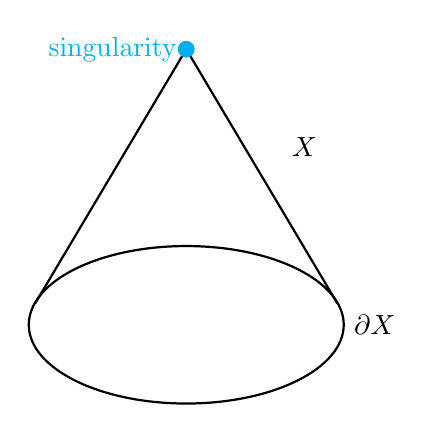
\begin{tikzpicture}
        \draw[thick] (0,0) -- (-1.92,-3.23);
        \draw[thick] (0,0) --  (1.92,-3.23) (1.5,-1.5) node[above]{$X$};
        \draw[thick] (0,-3.5) ellipse (2 and 1)  (2,-3.5) node[right]{$\partial X$};
        \filldraw[cyan] (0,0) circle (.1) (0,0) node[left]{singularity} ;
    \end{tikzpicture}
\end{center}

例如，若 $X$ 局部地是一组方程
\be  f_1(x_1,\dots ,x_n) = f_2(x_1,\dots ,x_n) = \dots =f_k(x_1,\dots ,x_n) =0\subset \bbR[x_1,\dots , x_n] \ee
的交集，则
% ==== 原文 PDF 第 40 页 ====
“边界”$\ptl X$ 由子空间
\be  f_1 = f_2 =\dots =f_k = \sum_{i=1}^n x_i^2 -\varepsilon^2 = 0  \ee
给出，它构成半径为 $\varepsilon$ 的 $S^{n-1}$。

现设 $\ptl X$ 光滑，且存在非平凡的挠拓扑闭链 $[\alpha]\in H_i(\ptl X,\bbZ)$，其挠阶为 $l$，使得 $l[\alpha]=0$。可以构造一个子锥 $\Sigma_{i+1}[\alpha]\subset X$，即 $[\alpha]$ 上的锥，如图~\ref{fig:cones} 所示。于是可以把高形式对称性下的带荷对象构造为绕 $\Sigma_{i+1}[\alpha]$ 缠绕的 M2 或 M5 膜\footnote{确切地说，$\Sigma_{i+1}[\alpha]\in \frac{H_{i+1}(X,\ptl X,\mb{Z})}{H_{i+1}(X,\mb{Z})}$，其中 $H_{i+1}(X,\ptl X,\mb{Z})$ 是 $(X,\ptl X)$ 的相对同调群。}，具体地说，

\begin{enumerate}
    \item 绕 $\Sigma_{i+1}[\alpha]$ 的 M2 膜在 $\bbZ_l^{(2-i)}$ 下带荷，即电的 $(2-i)$-形式对称性。
    \item 绕 $\Sigma_{i+1}[\alpha]$ 的 M5 膜在 $\bbZ_l^{(5-i)}$ 下带荷，即磁的 $(5-i)$-形式对称性。
\end{enumerate}

\begin{yizhu}
指数 $2-i$ 与 $5-i$ 来自维数计数，并非任取：锥 $\Sigma_{i+1}[\alpha]$ 的实维数为 $i+1$，M2 膜的世界体积为 3 维，绕锥缠绕后在 $\bbR^{d-1,1}$ 中留下的对象维数为 $3-(i+1)=2-i$；M5 膜的世界体积为 6 维，相应为 $6-(i+1)=5-i$。按本讲义的约定，$q$-形式对称性作用于 $q$ 维对象，故 M2、M5 分别给出电、磁两种对称性的带荷对象（M2 电耦合于 $C_3$，M5 磁耦合于对偶的 $C_6$）。更须注意 $[\alpha]$ 是挠闭链而非普通闭链：$\Sigma_{i+1}[\alpha]$ 是相对同调中的“锥”，其边界为 $[\alpha]$（脚注 9 用相对同调群把这一点说清楚），而 $l[\alpha]=0$ 正是群为 $\bbZ_l$ 而非 $\bbZ$ 的几何来源。
\end{yizhu}

注意，上述两个对称性由非对易的挠通量生成，且它们彼此并不局域\cite{DelZotto:2015isa,Albertini:2020mdx}。在良定义的（绝对）理论中，需要选择一个极化（polarization），这类似于 $SU(N)$ 规范理论的情形。也就是说，可以保留 M2 膜而得到电的 $(2-i)$-形式对称性，或保留 M5 膜而得到磁的 $(5-i)$-形式对称性。

\begin{yizhu}
“极化”指的是绝对理论中允许哪一族膜作为带荷对象：两族对称性生成元由非对易的挠通量给出、彼此不局域，因而不能在同一个绝对理论中同时存在。这与 $d=4$ 麦克斯韦理论中电、磁 1-形式对称性只能择一的情形同构（电磁对偶把两者互换），也类似 $SU(N)$ 规范理论中威尔逊线与 't Hooft 线的选择：一种选择对应电极化，另一种对应磁极化。选定 M2 后，M5 膜便成为该绝对理论中的非局域拓扑缺陷，反之亦然。原文所引文献中有关于非对易挠通量（non-commutative torsional flux）的专门讨论，可对照阅读。
\end{yizhu}

该机制也适用于 IIA/IIB 弦理论，此时带荷对象是 D$p$-膜而非 M2/M5 膜。

\begin{figure}[htbp]
    \centering
    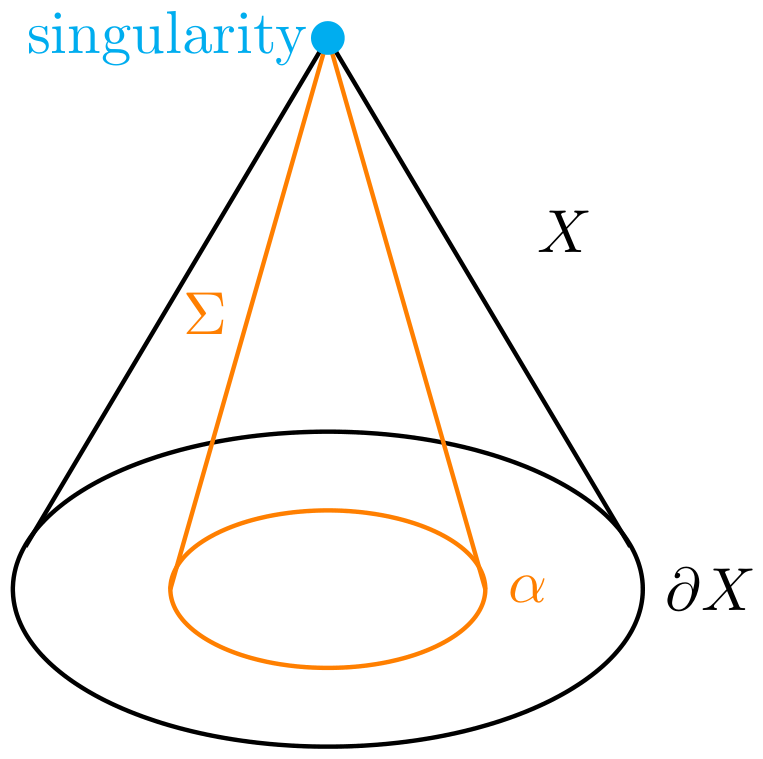
\includegraphics[width=0.30\linewidth]{figures/figure-7.png}
    % [原文图注为空]
    \caption{}
    \label{fig:cones}
\end{figure}

% ==== 原文 PDF 第 41 页 ====
\subsubsection{5 维 $\mathcal{N}=1$ 超共形场论}

在五维，一个重要的特征是：所有（超对称）规范理论在紫外都是强耦合的，例如杨–米尔斯作用量
\be  S_{YM} = \int \dd^5 x \frac{1}{g_{YM}^2} (F_{\mu\nu}F^{\mu\nu}) \ \Rightarrow \ [g_{YM} ] = -\frac{1}{2}  \ee
当能标 $\to\infty$ 时，$g_{YM}$（以该能标为单位）$\to0$，规范理论变得无限强耦合。在一定条件下，超对称规范理论可以紫外完备化为带有 8 个超荷的 $\cN=1$ 超共形场论（SCFT），例如可参见\cite{Seiberg:1996bd,Morrison:1996xf,Intriligator:1997pq,Aharony:1997bh,Benini:2009gi,Kim:2012gu,Bergman:2013aca,Zafrir:2014ywa,Hayashi:2015zka,Xie:2017pfl,Ferlito:2017xdq,Hayashi:2018lyv,Jefferson:2018irk,Bhardwaj:2018vuu,Closset:2018bjz,Cabrera:2018jxt,Apruzzi:2018nre,Bhardwaj:2018yhy,Apruzzi:2019vpe,Apruzzi:2019opn,Apruzzi:2019enx,Apruzzi:2019kgb,Bhardwaj:2019fzv,Bhardwaj:2020gyu,Eckhard:2020jyr,Bhardwaj:2020ruf,BenettiGenolini:2020doj,Bhardwaj:2020avz,Closset:2020scj,Closset:2021lwy,Tian:2021cif,Genolini:2022mpi,DelZotto:2022fnw,Collinucci:2022rii,DeMarco:2022dgh,Bourget:2023wlb}。

若在矢量多重态\footnote{超多重态是超对称代数的一个表示，由自旋不同的粒子组成。对于无质量矢量多重态，其中包含矢量场 $A_\mu$、马约拉纳旋量 $\chi$ 与实标量 $\phi$。} $(A_\mu,\chi,\phi)$ 中，实标量 $\phi$ 获得非零真空期望值（VEV，即 $\expval{\phi}\ne 0$），则这一非零 VEV 把原来的、可能非阿贝尔的规范理论/超共形场论破缺为 $U(1)^r$（$r$ 为原规范群的秩）阿贝尔规范理论，带电物质为超多重态\footnote{超多重态中包含一个马约拉纳旋量 $\psi$ 与两个复标量 $\phi$ 及 $\Tilde{\phi}$。} $(\psi,\phi,\Tilde{\phi})$。

这一点有 M 理论实现，我们在第~\ref{sssect:M-th}~节发展的工具正好用得上。考虑紧化在带有奇异点的 Calabi-Yau 三流形 $X$
\footnote{这里的 3 指复维数，就实维数而言是 6。Calabi-Yau 意味着其典范丛平凡。}
上的 11 维 M 理论。从紫外超共形场论到库仑分支（Coulomb branch）的过程，对应于 crepant 解奇（crepant resolution）\footnote{形式上，crepant 解奇是保持典范除子不变的双有理映射。}，即对奇异点作光滑化，同时保持场论的超对称性。

\begin{center}
    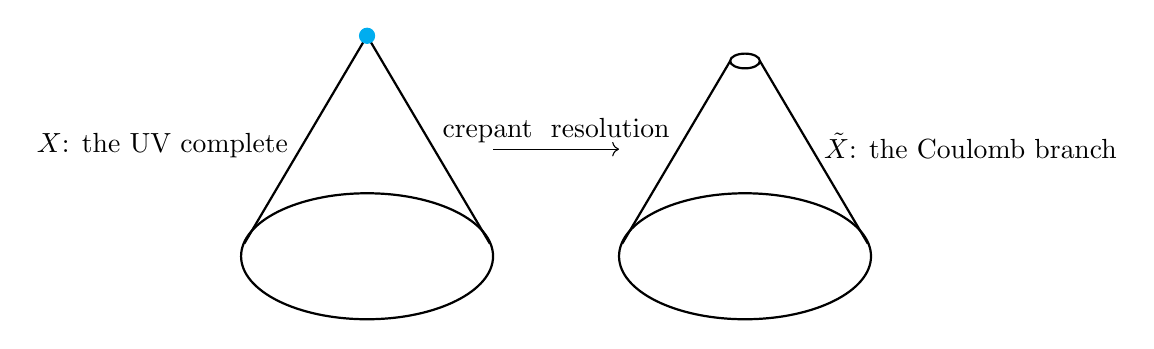
\begin{tikzpicture}[scale = 0.8]
        \draw[thick] (0,0) ellipse (2 and 1);
        \draw[thick] (1.95,0.2) -- (0,3.5)  (-1.95,0.2) -- (0,3.5) ;
        \filldraw[cyan]  (0,3.5) circle (0.12);
        \node at (3,2) { crepant \ resolution};
        \node at (-1.1,1.75) [left] {$X$: the UV complete};
        \node at (7.1,1.75) [right] {$\Tilde{X}$: the Coulomb branch};

        \draw[->] (2,1.7)--(4,1.7);
        \draw[shift = {(6,0)},thick] (0,0) ellipse (2 and 1);
        \draw[shift = {(6,0)},thick] (1.95,0.2)--(0.236,3.1) (-1.95,0.2)--(-0.235,3.1);
        \draw[shift = {(6,0)}, thick] (0,3.1) ellipse (0.236 and 0.117);
    \end{tikzpicture}
\end{center}

在解奇后的 $\Tilde{X}$ 中有紧致 4-闭链 $S_i \ (i\in {1,\cdots ,r})$，每个对应库仑分支上的一个规范群 $U(1)_i$。利用 M 理论 $C_3$ 规范场的展开
\be C_3 = \sum_{r=1}^r A_i \wedge \omega_i  \ee
其中 $\omega_i$ 是 $S_i$ 的庞加莱对偶 2-形式，$A_i$ 是 $U(1)_i$ 规范场。此外还有紧致 2-闭链 $C_j$，绕 $C_j$ 缠绕的 M2 膜给出 $5$ 维中的 BPS 粒子，其
% ==== 原文 PDF 第 42 页 ====
$U(1)_i$ 下的电荷定义为
\be q_{i,j} = {\rm Int}(C_j,S_i)|_{\Tilde{X}}\,,  \ee
即交点数。

\begin{yizhu}[原文疑误]
（4.7）的求和上下限与被加项指标不匹配：原文写作 $\sum_{r=1}^r A_i \wedge \omega_i$，上限用 $r$、被加项却用 $i$，按上下文应为 $\sum_{i=1}^r A_i\wedge\omega_i$（$r$ 为规范群的秩）；此处照原文保留。同段的“$S_i$ 的庞加莱对偶 2-形式”与后文“每个 $s_i$”大小写不一致（后者照原文保留为小写 $s_i$）。此外，源码把集合写成未转义花括号的 $1,\cdots ,r$，排出来是 $i\in 1,\cdots ,r$，应为 $\{1,\cdots ,r\}$，属排版瑕疵，不影响内容。
\end{yizhu}

在一定条件下，可以从 $\Tilde{X}$ 取几何极限。假设每个 $s_i$ 具有 $S^2$-纤维化结构，并取 ${\rm vol}(S^2)\to 0$ 的极限。其图像是：这是非阿贝尔规范理论的极限，因为绕 $S^2$ 的 M2 膜就是 W-玻色子，所以把体积取为零就使相应（关于指标 $i$）的 W-玻色子变为无质量。这与 5 维非阿贝尔规范理论的红外物理描述一致。

作为一个详细的例子，考虑环面（toric）CY3 奇点 $X$ 的情形，它是 Sasaki-Einstein 五维流形\footnote{Sasaki-Einstein 流形 $X$ 定义为度规锥 $\mb{R}_{>0}\times X$ 为 K\"ahler 且 Ricci 平坦的流形\cite{Sparks:2010sn}。对于 $Y^{N,k}$，它可以描述为 $S^2\times S^2$ 上的 $S^1$-丛，其第一陈类 $c_1$ 由 $N$ 与 $k$ 参数化。} $Y^{N,k}$ 上的锥。我们把 $X$ 的 crepant 解奇画成环面图（关于环面 CY3 的记号，例如可参见\cite{Xie:2017pfl,Eckhard:2020jyr}）

\begin{center}
    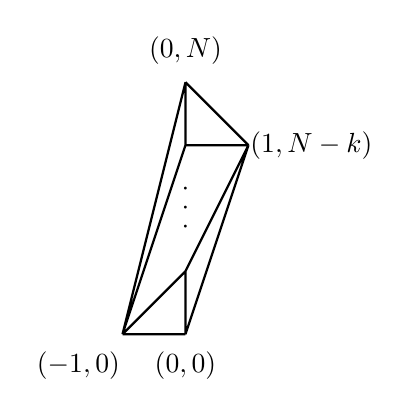
\begin{tikzpicture}[scale = 0.8]
        \draw[thick] (0,1) -- (0,2) (0,1)-- (1,1) (0,2) -- (1,1) (0,2) -- (-1,-2) (0,1) -- (-1,-2) (0,-1) -- (0,-2) (0,-1) -- (1,1) (0,-2) -- (1,1) (0,-1) -- (-1,-2) (0,-2) -- (-1,-2);
        
        \node at (0,2.5) { $(0,N)$};
        \node at (0,-2.5) { $(0,0)$};
        \node at (-1.7,-2.5) { $(-1,0)$};
        \node at (2,1) { $(1,N-k)$};
        \node at (0,0.3) { $\cdot$};
        \node at (0,0) { $\cdot$};
        \node at (0,-0.3) { $\cdot$};
    \end{tikzpicture}
\end{center}

紧致除子 $S_i$（$i=1,\dots,N-1$）都是底为 $S^2$、纤维为 $S^2$ 的纤维化。该理论在红外有非阿贝尔规范理论描述 $SU(N)_k$，其中 $k$ 是陈–西蒙斯能级。

可以用三种不同的方法计算 1-形式对称性，结果彼此相同。这里选择极化，使给定的几何设定具有最大的 1-形式对称性。

\begin{enumerate}
\item{可以计算电荷矩阵 $q_{i,j}$ 的 Smith 标准形（Smith normal form），见 \ref{SmithDecomp}。由 Smith 标准形可读出 1-形式对称性 $\Gamma^{(1)}=\mb{Z}_{\text{gcd}(N,k)}$。}
\item{从链环（link）五维流形 $Y^{N,k}$ 的同调，有
\be
\ba
&H_0(Y^{N,k},\mb{Z})=\mb{Z}\ ,\ H_1(Y^{N,k},\mb{Z})=\mb{Z}_{\text{gcd}(N,k)}\ ,\ H_2(Y^{N,k},\mb{Z})=0\ ,\ \cr
&H_3(Y^{N,k},\mb{Z})=\mb{Z}_{\text{gcd}(N,k)}\ ,\ H_4(Y^{N,k},\mb{Z})=0\ ,\ 
H_5(Y^{N,k},\mb{Z})=\mb{Z}\,.
\ea
\ee
}
\item{从场论论证，$SU(N)$ 的 1-形式中心对称性 $\mb{Z}_N$ 被 5 维陈–西蒙斯项破缺为子群 $\mb{Z}_{\text{gcd}(N,k)}$。}
\end{enumerate}

% ============================================================
% 片段：s04b  对应原文 section2.tex 第 1198--1468 行；PDF 第 43--49 页
% 内容：§4.2 在凝聚态物理中的应用（4.2.1 环面码模型；4.2.2 3+1 维的 SPT）
% 译者：t-s04b   审校状态：初稿
% ============================================================

% ==== 原文 PDF 第 43 页 ====
\subsection{在凝聚态物理中的应用}\label{sec:appl-CMP}

研究广义对称性的一个自然框架，由具有任意子激发的 2+1 维拓扑序提供；这些系统在凝聚态物理领域已被广泛研究。它们在数学上由幺正模张量范畴描述，后者为刻画任意子的融合与编织结构提供了强有力的形式体系\cite{KITAEV20062}。这些系统中任意子所扫出的世界线，可以解释为该系统的拓扑缺陷线（topological defect line，TDL）。这类算符的关键之处在于：与作用于整个系统的整体对称性作用不同，它们只作用于系统中一部分自由度\cite{PhysRevB.72.045137,pnas.0803726105,NUSSINOV2009977}。在这个意义上，它是逐点作用于系统的规范对称变换的推广。

当任意子为阿贝尔任意子时，系统中的所有 TDL 都是可逆的。此时，由任意子世界线生成的对称性对应于 1-形式对称性。反之，若任意子是非阿贝尔的（这意味着 TDL 非可逆），则与任意子世界线相联系的对称性就是非可逆对称性。

为说明这些概念，我们以著名的环面码模型（toric code model）作为具体例子。我们将证明，这个 2+1 维系统中由任意子世界线产生的 1-形式对称性是反常的。此外，我们还将说明，这个带有反常 1-形式对称性的系统可以作为 3+1 维 1-形式 SPT 态的边界而被实现。

\subsubsection{环面码模型}

环面码模型\cite{KITAEV20032}是规范群为 $\mathbb{Z}_2$ 的 2+1 维格点规范理论的一个著名例子。该模型中，我们考虑具有正方格子的二维空间，其中每条格点边（link）都赋予一个自旋-$1/2$ 自由度。系统的希尔伯特空间是每条边对应的复二维向量空间 $\mathbb{C}^2$ 的张量积：
\be
\mathcal{H} = \bigotimes_{\text{每条边}} \mathbb{C}^2.
\ee

我们在环面码模型中定义如下两类算符：
\begin{center}
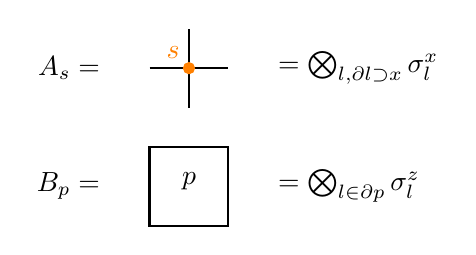
\begin{tikzpicture}
    \draw[thick] (-0.5,0)--(0.5,0) (-1,0)node[left]{$A_s = $};
    \draw[thick] (0,-0.5)--(0,0.5) (1,0) node[right]{$ = \bigotimes_{l, \ptl l\supset {x}} \sigma^{x}_{l}$};
    \filldraw[orange] (0,0) circle (2pt) (-0.2,0)node[above]{$s$};
    \draw[thick] (-0.5,-2) rectangle (0.5,-1) (-1,-1.5)node[left]{$B_p = $} (0,-1.2)node[below]{$p$} (1,-1.5)node[right]{$ = \bigotimes_{ l\in \ptl p} \sigma^{z}_{l}$};
\end{tikzpicture}
\end{center}

其中每个顶点（vertex）记为 $s$，每个面（plaquette）记为 $p$。
% ==== 原文 PDF 第 44 页 ====
不难验证这些算符具有如下性质
\be\ba 
A_s^\dag &= A_s,  \ \ A_s^2 = 1 \Rightarrow \ {\rm Spec}(A_s) = {\pm 1} ,\\ 
B_p^\dag &= B_p, \ \ B_p^2 = 1 \Rightarrow \ {\rm Spec}(B_p) = {\pm 1} ,\\
[A_s,A_{s'}] &= [B_p,B_{p'}]= [A_s,B_p]  = 0 , \ \forall s,s',p,p' .
\ea\ee

环面码模型的哈密顿量是与 $A_s$ 及 $B_p$ 算符相关联的所有相互对易的投影算符项之和，即：
\be
H = -\left(\sum_{s} A_s + \sum_{p} B_p\right).
\ee

由于哈密顿量中所有项彼此对易，我们可以容易地确定该模型的全部能谱：
\be\ba
\text{基态} &:  A_s\ket{0} = B_p\ket{0} = \ket{0} \\
\text{激发态} &: A_s \ket{\Psi} = -\ket{\Psi}, \text{ 或 } B_p \ket{\Psi} = -\ket{\Psi},  \ \text{对某些 }s,p
\ea\ee

这简化了寻找基态与激发态的过程，使得分析环面码模型的行为并研究其激发变得可行。

环面码模型与电磁学之间存在直观的对应关系，后者由 $U(1)$（格点）规范理论描述。
\begin{center}
    \begin{tabular}{ccc}
        离散 $\bbZ_2$ 规范理论 & $\longrightarrow$  &  $U(1)$ 规范理论  \\
        $\sigma^z_l$ &   $\longrightarrow$  &  威尔逊线 $\exp(i\int A_{ij})$  \\
        $B_p$ &   $\longrightarrow$  &  $\exp(i\oint A)=  \exp(i\int F) \sim \exp(ia^2 B) $  \\
        $\sigma^x_{l}$ &   $\longrightarrow$  &  $\exp(i\int_l E)$  \\
        $A_s$ &   $\longrightarrow$  & $\exp(i \nabla\cdot E)$   \\
        $H = -(\sum_s A + \sum_p B)$ &   $\longrightarrow$  &  $\vb{B}^2 + (\nabla\cdot \vb{E})^2$  \\
        $B_p = \pm 1$ &  $\longrightarrow$   &  $ \int B =0 \ / \ \ne 0$  \\
        $A_s = \pm 1$ &   $\longrightarrow$  &  $\nabla E = 0\ / \ \ne 0$  \\

    \end{tabular}
    \label{tab:Z2U1}
\end{center}

\begin{yizhu}该表是“离散 $\Z_2$ 规范理论与连续 $U(1)$ 规范理论”之间的对照词典，读表时须分清两类角色：开弦 $\sigma^z_l$ 对应威尔逊线，按 (4.21) 它是 $\Z_{2,M}^{(1)}$ 的带荷对象；与它对偶的 't Hooft 线 $\sigma^x_{l}$ 则是 $\Z_{2,E}^{(1)}$ 的带荷对象。而闭圈 $B_p$ 与 $A_s$ 分别是 $\Z_{2,E}^{(1)}$、$\Z_{2,M}^{(1)}$ 的对称性算符：由 (4.14) 可见 $B_p$ 只与 $W_M$ 的端点（$p\in\partial L^\ast$ 处）反对易，$A_s$ 只与 $W_E$ 的端点（$s\in\partial L$ 处）反对易。表中 $B_p$ 一行写作 $\exp(i\oint A)$（闭威尔逊圈，而不是威尔逊线）并等价于 $\exp(ia^2B)$，正是这一对偶互换的体现：在环面码中，一个 1-形式对称性的生成元恰是另一个 1-形式对称性的带荷算符。\end{yizhu}

这一对应关系还有助于我们构造环面码模型中的激发。1-形式对称性可以通过与这些激发相联系的弦算符（string operator）来理解，如下图所示：

% ==== 原文 PDF 第 45 页 ====
\begin{center}
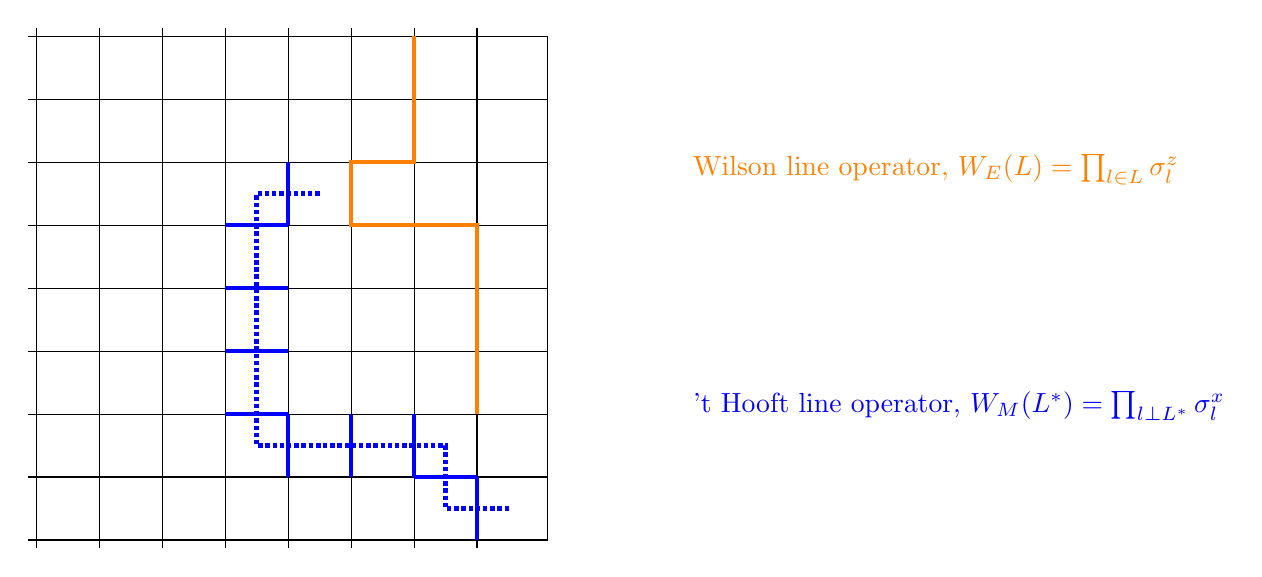
\begin{tikzpicture}
    \draw[] (-3.3,3.2)--(3.3,3.2);
    \draw[shift = {(0,-0.8)}] (-3.3,3.2)--(3.3,3.2);
    \draw[shift = {(0,-1.6)}] (-3.3,3.2)--(3.3,3.2);
    \draw[shift = {(0,-2.4)}] (-3.3,3.2)--(3.3,3.2);
    \draw[shift = {(0,-3.2)}] (-3.3,3.2)--(3.3,3.2);
    \draw[shift = {(0,-4.0)}](-3.3,3.2)--(3.3,3.2);
    \draw[shift = {(0,-4.8)}](-3.3,3.2)--(3.3,3.2);
    \draw[shift = {(0,-5.6)}](-3.3,3.2)--(3.3,3.2);
    \draw[shift = {(0,-6.4)}](-3.3,3.2)--(3.3,3.2);
    \draw[] (3.3,-3.2)--(3.3,3.2);
    \draw[shift = {(-0.8,0)}] (3.2,-3.3)--(3.2,3.3);
    \draw[shift = {(-1.6,0)}] (3.2,-3.3)--(3.2,3.3);
    \draw[shift = {(-2.4,0)}] (3.2,-3.3)--(3.2,3.3);
    \draw[shift = {(-3.2,0)}] (3.2,-3.3)--(3.2,3.3);
    \draw[shift = {(-4.0,0)}] (3.2,-3.3)--(3.2,3.3);
    \draw[shift = {(-4.8,0)}] (3.2,-3.3)--(3.2,3.3);
    \draw[shift = {(-5.6,0)}] (3.2,-3.3)--(3.2,3.3);
    \draw[shift = {(-6.4,0)}] (3.2,-3.3)--(3.2,3.3);
    \draw[orange, ultra thick]  (1.6,3.2)--(1.6,2.4)--(1.6,1.6)--(0.8,1.6)--(0.8,0.8)--(1.6,0.8)--(2.4,0.8)--(2.4,-1.6) (5,1.5)node[right]{Wilson line operator, $W_E(L) = \prod_{l\in L} \sigma^z_l  $};
    \draw[blue,ultra thick, densely dotted] (0.4,1.2)--(-0.4,1.2)--(-0.4,0.4)--(-0.4,-0.4)--(-0.4,-1.2)--(-0.4,-2.0)--(0.4,-2.0)--(1.2,-2.0)--(2.0,-2.0)--(2.0,-2.8)--(2.8,-2.8);
    \draw[blue,ultra thick] (0,0.8)--(0,1.6)     (5,-1.5)node[right]{'t Hooft line operator, $W_M(L^*) = \prod_{l\perp L^*} \sigma^x_l$};
    \draw[blue,ultra thick] (0,0.8)--(-0.8,0.8);
    \draw[shift = {(0,-0.8)},blue,ultra thick] (0,0.8)--(-0.8,0.8);
    \draw[shift = {(0,-1.6)},blue,ultra thick] (0,0.8)--(-0.8,0.8);
    \draw[shift = {(0,-2.4)},blue,ultra thick] (0,0.8)--(-0.8,0.8);
    \draw[shift = {(2.4,-3.2)},blue,ultra thick] (0,0.8)--(-0.8,0.8);

    \draw[shift = {(0,-3.2)},blue,ultra thick] (0,0.8)--(0,1.6);
    \draw[shift = {(0.8,-3.2)},blue,ultra thick] (0,0.8)--(0,1.6);
    \draw[shift = {(1.6,-3.2)},blue,ultra thick] (0,0.8)--(0,1.6);
    \draw[shift = {(2.4,-4)},blue,ultra thick] (0,0.8)--(0,1.6) ;
    
\end{tikzpicture}
\end{center}

在如上定义了威尔逊线与 't Hooft 线算符之后，可以证明它们的对易子为（当存在非零交点时）
\be\ba
[ W_E(L), B_p ] &= 0,  \ \ [W_M(L^*),B_p]\ne 0 \text{ iff } p\in\partial L^\ast \\
[W_E(L),A_s]&\ne 0 \text{ iff }s\in \partial L, \ \ [W_M(L^*), A_s] = 0  \\
[W_E(L) ,H] &= [W_M(L^*),H] = 0 \ {\rm if} \ \ptl L = \partial L^\ast=  0\\
[W_E(L), W_M(L^*) ] &= 0  \ , \ {\rm if \ } L \cap L^\ast = 0 
\ea\ee

现在可以陈述如下事实：\textbf{环面码系统的激发是开线算符的端点。}更具体地，有
\be
 \ba
s &\notin \ptl L \  : \ A_s W_E(L) \ket{0} = W_E(L) A_s \ket{0} =  W_E(L) \ket{0} \\
s &\in \ptl L \ : \ A_s W_E(L) \ket{0} = -W_E(L) A_s \ket{0} =  -W_E(L) \ket{0}
\ea  \ee

因此，电荷 $e$ 是威尔逊线的端点。类似地，对磁的部分，有
\be
 \ba
p &\notin \ptl L^* \  : \ B_p W_M(L) \ket{0} = W_M(L^*) B_p \ket{0} =  W_M(L^*) \ket{0} \\
p &\in \ptl L^* \ : \ B_p W_M(L) \ket{0} = -W_M(L^*) B_p \ket{0} =  -W_M(L^*) \ket{0}
\ea   \ee

因此，磁荷 $m$ 是 't Hooft 线端点处的激发。

与开线给出激发的情形相反，闭圈是用于对简并态分类的守恒荷。我们关心的是基态。设该格点的整体结构为环面 $T^2 = S^1\times S^1$，则有两类非平凡圈。考虑 $W_E(L_{1,2}) = \pm 1$ 或 $W_M(L_{1,2})=\pm 1$，简并度至少为 4。

\begin{yizhu}基态简并度“至少为 4”的理由可用逻辑算符来说明：在 $T^2$ 上，$W_E$ 与 $W_M$ 各有两个不可收缩的闭圈，即 $W_E(L_1),W_E(L_2)$ 与 $W_M(L_1^\ast),W_M(L_2^\ast)$；它们都与 $H$ 对易，但电型闭圈与磁型闭圈之间互不对易，且 $W_E^2=W_M^2=1$。因此在基态子空间上可以同时取两组独立的 $\pm1$ 本征值，给出 $2^2=4$ 维基态空间；对亏格 $g$ 的曲面应推广为 $2^{2g}$。注意这些闭圈正是非定域的逻辑算符，与开弦端点处的任意子激发 $e$、$m$、$em$ 是不同对象。\end{yizhu}

通过在二维空间流形的希尔伯特空间上对泡利矩阵作简单计算，可以看出
\be\label{EM} W_E(L) W_M(L^*) = (-1)^{{\rm Int}(L,L^*)}   W_M(L^*)W_E(L), \ee

这意味着 't Hooft 线是威尔逊线所作用的对象，反之亦然。这里 $\mathrm{Int}(L,L^\ast)$ 是二维空间流形上两条线 $L$ 与 $L^\ast$ 的交点数。至此，我们已准备好讨论激发的统计性质。

% ==== 原文 PDF 第 46 页 ====
若同时考虑时间维度，这些线现在便画在 2+1 维时空之中。由于沿同一链的 $\sigma_l^x$ 与 $\sigma_l^z$ 反对易，交换两条线的次序会产生一个负号。这一概念可用下图直观地表示：
\begin{center}
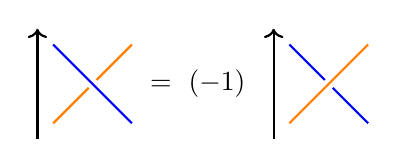
\begin{tikzpicture}
    \draw[orange , thick ] (0,0)--(0.45,0.45)  (0.55,0.55)--(1,1);
    \draw[blue, thick]  (1,0)--(0,1);
    \draw[thick , -> ] (-0.2,-0.2)--(-0.2,1.2);
    \draw[thick] (-0.2,0)--(-0.2,1) (1.1,0.5)node[ right]{$= \ (-1)$};
    \draw[shift = {(3,0)},thick , -> ] (-0.2,-0.2)--(-0.2,1.2);
    \draw[shift = {(3,0)},orange ,thick] (0,0)--(1,1);
    \draw[shift = {(3,0)},blue, thick] (0,1)--(0.45,0.55) (0.55,0.45)--(1,0);
\end{tikzpicture}
\end{center}

这蕴含着该系统的阿哈罗诺夫–玻姆效应（Aharonov-Bohm effect）
\begin{center}
    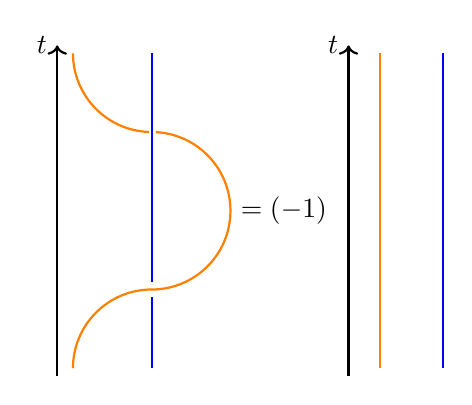
\begin{tikzpicture}
        \draw[thick,->] (-0.20,-0.1)--(-0.20,4.1) node[left]{$t$};
        \draw[shift = {(3.7,0)},thick,->] (-0.20,-0.1)--(-0.20,4.1) node[left]{$t$};

        \draw[thick] (-0.20,0)--(-0.20,1) (2,2)node[right]{$= (-1)$};
        \draw[orange,thick] (0,0) arc (180:90:1) (1,1) arc (-90:87:1) (0,4) arc (180:268:1);
        \draw[thick, blue] (1,0)--(1,0.9) (1,1.1)--(1,4);
        \draw[shift = {(3.7,0)},thick, blue] (1,0)--(1,4) ;
        \draw[shift = {(3.7,0)},thick, orange] (0.2,0)--(0.2,4) ;

    \end{tikzpicture}.
\end{center}

以及，如果把线的端点闭合成圈，一个 Hopf 链环的取值：
\begin{center}
    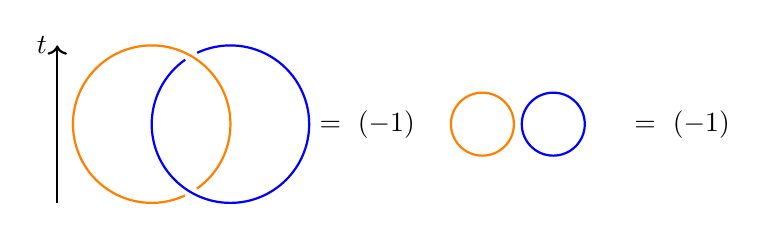
\begin{tikzpicture}
        \draw[thick , orange] (1,0) arc (0:295:1) (1,0) arc (0:-55:1) ;
        \draw[thick , blue] (2,0) arc (0:-235:1) (2,0) arc (0:115:1);
        \draw[thick,->] (-1.2,-1)--(-1.2,1) node[left]{$t$};
        \draw[thick] (-1.2,0)--(-1.2,0.1) (2.0,0) node[right]{$= \ (-1)$} (6,0) node[right]{$= \ (-1)$} ;
        \draw[shift = {(1.6,0)},thick , orange] (3,0) arc (0:360:0.4) ;
        \draw[shift = {(2,0)},thick , blue] (3.5,0) arc (0:360:0.4) ;
      
    \end{tikzpicture}
\end{center}


从高形式对称性的角度看，2+1 维环面码模型显然具有 $\mathbb{Z}_{2,E} \times \mathbb{Z}_{2,M}$ 1-形式对称性，其特征如下：
\be\ba
\bbZ_{2,E}^{(1)}: W_E(L) W_M(L^*) &= (-1)^{{\rm Link}(L,L^*)}  W_M(L^*), \\
\bbZ_{2,M}^{(1)}: W_M(L^\ast) W_E(L) &= (-1)^{{\rm Link}(L^\ast,L)}  W_E(L) .
\ea\ee

这些方程应在 2+1 维时空的语境下理解，而不是如式~(\ref{EM}) 那样在二维空间的语境下理解。值得注意的是，对这两个不同的 1-形式对称性而言，威尔逊线算符与 't Hooft 线算符的角色可以互换：一个充当 1-形式对称性算符，另一个则是其带荷算符。

\begin{yizhu}(4.14) 与 (4.17) 的对易关系是弦算符与格点算符作用次序的直接推论：$W_E(L)$ 是沿链 $L$ 的 $\sigma^z_l$ 之积，因此只有当 $A_s=\prod_{l\ni s}\sigma^x_l$ 的支撑与 $L$ 在端点 $s\in\partial L$ 处重叠时才会出现反对易；同理，$W_M(L^\ast)$ 只在 $p\in\partial L^\ast$ 处与 $B_p$ 反对易。所有 $(-1)$ 因子的唯一来源是同一链上 $\sigma_l^x\sigma_l^z=-\sigma_l^z\sigma_l^x$，即每条边上的自旋-$1/2$ 自由度，这也解释了为何这些对易子只能取 $\pm1$。另须注意维数：(4.17) 写在二维空间中，因子是 $(-1)^{\mathrm{Int}(L,L^\ast)}$；而 (4.18) 写在 2+1 维时空中，因子是 $(-1)^{\mathrm{Link}(L,L^\ast)}$。把其中一条线提升为时间方向的世界线后，二者是同一个拓扑量，但对易子的计算语境不可混用。\end{yizhu}

% ==== 原文 PDF 第 47 页 ====
这把我们引向该 1-形式对称性的反常问题。事实上，这两个 $\Z_2$ 1-形式对称性具有混合 't Hooft 反常。它可以从三个不同视角来理解：
\begin{enumerate}
    \item 威尔逊圈与 't Hooft 圈在 2+1 维时空中的构型，对应于 1-形式对称性的一个缺陷网络。由于这两个 $\Z_2$ 1-形式对称性彼此不同，它们的缺陷线应当保持相互独立。然而，如前文所讨论的，该缺陷网络在本质上不是拓扑的：
    \be
    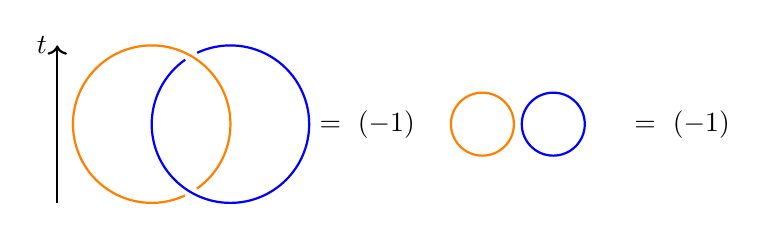
\begin{tikzpicture}
    \label{grf:link}
        \draw[thick , orange] (1,0) arc (0:295:1) (1,0) arc (0:-55:1) ;
        \draw[thick , blue] (2,0) arc (0:-235:1) (2,0) arc (0:115:1);
        \draw[thick,->] (-1.2,-1)--(-1.2,1) node[left]{$t$};
        \draw[thick] (-1.2,0)--(-1.2,0.1) (2.0,0) node[right]{$= \ (-1)$} (6,0) node[right]{$= \ (-1)$} ;
        \draw[shift = {(1.6,0)},thick , orange] (3,0) arc (0:360:0.4) ;
        \draw[shift = {(2,0)},thick , blue] (3.5,0) arc (0:360:0.4) ;
      
    \end{tikzpicture}
\ee
    这一现象可以理解为一种混合反常，类似于前文提到的 1+1 维情形中结合律的破坏。
    \item 另一个考察反常的视角是通过规范变换。环面码的作用量可以写成一个陈–西蒙斯理论
    \be S = \int_{M_3}  \frac{2}{2\pi} b^{(1)}\wedge \dd a^{(1)}  \ee
    其中威尔逊线与 't Hooft 线算符为
    \be\left\{ \ba
    W_E(L) &= \exp(i\int_L a),  \ \ \ \ \bbZ_{2,M}^{(1)}\ \text{带荷算符} \\
    W_M(L) &= \exp(i\int_L b), \ \  \ \ \bbZ_{2,E}^{(1)}\ \text{带荷算符} 
    \ea \right. \ee
    现在，若把该理论与背景 2-形式规范场（记为 $B_{E,M}^{(2)}$）耦合，试图对 $\bbZ_{2,E}^{(1)}\times \bbZ_{2,M}^{(1)}$ 1-形式对称性作规范化，则得到如下作用量
    \be S = \int_{M_3}  \frac{2}{2\pi} b^{(1)}\wedge \dd a^{(1)}  + \int_{M_3} \frac{1}{2\pi} (a^{(1)}\wedge B_M^{(2)}+ b^{(1)}\wedge B_E^{(2)}). \ee
    在 $\bbZ_{2,E}^{(1)}$ 规范变换
    \be\left \{ \ba
    B_E &\mapsto B_E - \dd \chi \\
    a &\mapsto a+ \frac{1}{2} \chi 
    \ea \right. \ee
    之下，由于第二项，作用量显然不是规范不变的，尽管其余两项保持不变。类似地，对磁规范变换，
% ==== 原文 PDF 第 48 页 ====
    作用量也同样缺乏规范不变性。然而，若把该理论与一个 3+1 维体（bulk）耦合，其作用量为
    \be\label{eq:Sbulk} S_{\rm bulk} = \frac{1}{4\pi^2}\int_{M_4} B_E \wedge B_M, \ee
    则发现总理论变为规范不变的，这表明两个 1-形式对称性的混合反常由高一维的上述反常多项式所支配。
    \item 从分类空间的视角看，把两个规范场视为从时空到分类空间的映射：
    \be B,B': M_3 \to B^2(\bbZ_{2,E}\times \bbZ_{2,M} ) \ .\ee
    设这两个规范场映射分别对应于式~\ref{grf:link} 中非平凡链环与平凡链环的左右两侧缺陷网络构型。由于这两个 1-形式对称性彼此独立，两种构型的映射是同伦的。在无反常的理论中，两种构型的配分函数应当相同。然而在此情形下，式~\ref{grf:link} 中两种构型的配分函数相差一个 $(-1)$ 因子，这标志着混合反常的存在。
\end{enumerate}

\subsubsection{3+1 维的 $\bbZ_{2,E}^{(1)}\times \bbZ_{2,M}^{(1)}$ SPT}

为深化对前述 $\bbZ_{2,E}\times \bbZ_{2,M}$ 1-形式对称性反常的理解，可以尝试从 3+1 维 1-形式 SPT 的视角来认识它。3+1 维 $\bbZ_{2,E}^{(1)}\times \bbZ_{2,M}^{(1)}$ SPT 由下式分类
\be\ba  
H^4( B^2 \bbZ_{2,E}\times  B^2\bbZ_{2,M} ,U(1)) &\supset H^2(B^2 \bbZ_{2,E} , H^2( B^2\bbZ_{2,M} , U(1))) \\
&\cong  H^2(B^2 \bbZ_{2,E} ,\bbZ_2) \cong \bbZ_2 .
\ea\ee

它是上同调群的谱序列计算中的一项。值得注意的是，这一 $\bbZ_2$ 分类由项 $B_E^{(2)}\wedge B_M^{(2)}$ 生成。由此得到的 3+1 维 SPT 作用量表示为：
\be S_\mathrm{SPT} = \frac{1}{4\pi^2}\int_{M_4} B_E \wedge B_M.  \ee

这一结果恰好印证了式~(\ref{eq:Sbulk}) 中详述的反常多项式方法。本质上，它再次确认：2+1 维中两个 1-形式对称性的混合反常，可以通过由两个 2-形式规范场之楔积所刻画的 3+1 维 SPT 来理解。

\begin{yizhu}(4.26) 是上同调群的谱序列计算中的一项：对 $G=B^2\bbZ_{2,E}\times B^2\bbZ_{2,M}$，$H^4(BG,U(1))$ 由 Leray（Atiyah–Hirzebruch）谱序列的 $E_2^{p,q}=H^p(B^2\bbZ_{2,E},H^q(B^2\bbZ_{2,M},U(1)))$ 项逼近，作者给出的是 $p=q=2$ 这一项，即 $H^2(B^2\bbZ_{2,E},\bbZ_2)\cong\bbZ_2$，它由 $B_E^{(2)}\wedge B_M^{(2)}$ 生成。这里的 $\supset$ 表示它只是整个 $H^4$ 的一部分，其余 $(p,q)$ 项一般还可给出别的分类项；本例中该 SPT 的完整分类恰为 $\bbZ_2$。此外，$S=\frac{1}{4\pi^2}\int_{M_4}B_E\wedge B_M$ 的归一化要求 $B_{E,M}$ 是 $U(1)$ 联络的场强，即 $\oint B\in2\pi\bbZ$；在此归一化下 $\exp(iS_{\rm SPT})=(-1)^{nm}$，其中 $n,m$ 分别是 $B_E$、$B_M$ 在两个对偶 2-闭链上的通量整数。核对时应与 (4.22) 中的 $\frac{1}{2\pi}$ 耦合系数一并检查。\end{yizhu}

% ==== 原文 PDF 第 49 页 ====
现在，我们从拓扑缺陷网络的观点来考察：体作用量与边界作用量的反常为何相互抵消。2+1 维中的线算符可以自然地延拓为 3+1 维体中的面算符。由于总时空维数为四，两个这样的面算符的交集出现在 3+1 维时空中的离散点处。应用庞加莱对偶（Poincaré duality），这一交集可以等价地理解为 $B_E$ 与 $B_M$ 楔积的积分：
\be  B_E\wedge B_M \stack{\text{Poincar\'{e} 对偶}}{\longleftrightarrow} S_E\cap S_M. \ee

因此，3+1 维 1-形式 SPT 的作用量本质上是在数两个与 2-形式规范场对偶的面之间交点数的奇偶性。

这一几何解释漂亮地阐明了体与边界作用量之间反常的抵消。事实上，当我们试图把 2+1 维时空中的一个 Hopf 链环构型（如式~\ref{grf:link} 左侧所示）延拓到高一维时，最直接的延拓是到 4+1 维中的一个面，这将涉及单个交点。按此几何推理，体与边界理论合并后的整体是无反常的：
\be  (-1)^{\text{3+1 维中的交点数}} \cdot (-1)^{\text{2+1 维中的环绕数}} = 1.  \  \ee

由这一视角，我们完全从几何上理解了反常的抵消。

\begin{center}
    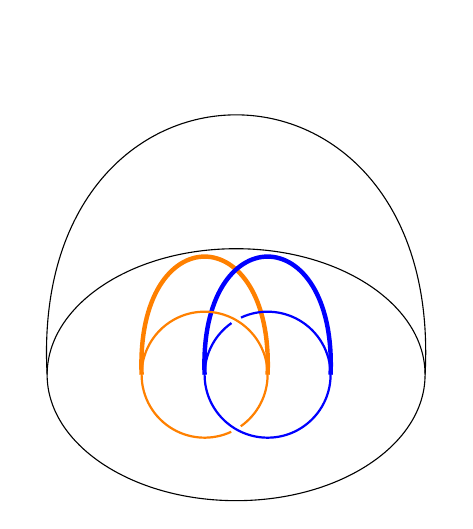
\begin{tikzpicture}[scale = 0.8]
        \draw (0.5,0) ellipse (3 and 2);
        \draw[shift = {(0.5,0)}] (-3,0) .. controls (-3.3, 5.5) and (3.3,5.5) .. (3,0);
        \draw[ultra thick, orange] (-1,0) .. controls (-1.1,2.5) and (1.1,2.5) .. (1,0);
        \draw[shift = {(1,0)},ultra thick, blue] (-1,0) .. controls (-1.1,2.5) and (1.1,2.5) .. (1,0);

        \draw[thick , orange] (1,0) arc (0:295:1) (1,0) arc (0:-55:1) ;
        \draw[thick , blue] (2,0) arc (0:-235:1) (2,0) arc (0:115:1);

    \end{tikzpicture}
\end{center}

还可以通过考察 1-形式 SPT 及其边界模型的具体格点模型来进一步加深理解。这使我们能够更细致地研究体对称性算符如何与边界算符相互作用，以及反常抵消如何发生。关于 $\mathbb{Z}_N$ 1-形式对称性的一个示例见文献\cite{PhysRevB.101.035101}。

\begin{yizhu}[原文疑误]原文此处写“the most straightforward extension to a surface in 4+1D”，与同段 (4.29) 中的“3+1D”以及全节始终在 3+1 维体中讨论的事实不一致：2+1 维时空中的两条线延拓一维后是 3+1 维时空中的两个面，而正是两个面在 3+1 维时空中才一般交于离散点（若真到 4+1 维，两个面一般交于 1 维曲线，不会给出“单个交点”）。此处照原文保留“4+1D”，疑应为“3+1D”。\end{yizhu}

% ==== 原文 PDF 第 49 页内容至此结束；第 50 页起为第 5 节（属其他片段）====

% ============================================================
% 片段：s05a  对应原文 section3.tex 第 1--307 行；PDF 第 50--58 页
% 内容：§5 Higher Group Symmetry（5.1 A Touch of Category Theory；5.2 Towards Defining a 2-Group）
% 译者：t-s05a   审校状态：初稿
% ============================================================

% ==== 原文 PDF 第 50 页 ====
\section{高群对称性}\label{sec:higher-group}

\begin{keytakeaways}
  \begin{itemize}[leftmargin=1.4em,itemsep=2pt,topsep=2pt]
    \item \textbf{物理图像}：普通规范理论用群元素标记点粒子的世界线；若要描述弦的世界面，就需把群升级为 2-群——1-态射标记世界线，2-态射标记世界面，这正是“高群对称性”的范畴论来源。
    \item \textbf{数学工具}：范畴（对象、态射、恒等、复合、结合律）$\to$ 群胚 $\to$ 函子；2-范畴（1-态射、2-态射、水平/垂直复合、交换律）$\to$ 2-群胚；交叉模作为严格 2-群的显式替代。
    \item \textbf{关键结论}：群等同于单对象群胚，其几何实现给出分类空间 $BG$；和乐 ${\rm hol}:\mathcal{P}_1(M)\to G$ 是函子，平凡 $G$-丛上的联络与光滑函子一一对应（定理~\ref{Thm:GaugeTh}）。
    \item \textbf{关键结论}：严格 2-群与交叉模 $(G,H,\ptl,\rhd)$ 一一对应；两条约束 $\ptl(g\rhd h)=g(\ptl h)g^{-1}$、$\ptl h\rhd h'=hh'h^{-1}$ 由 2-范畴的交换律直接推出，并非额外公设。
  \end{itemize}
\end{keytakeaways}

本章用范畴论的语言给出推广对称性的另一种方式。我们将看到如何把群描述为一个 1-范畴，以及如何把它推广到更高范畴的语言中。

对于更关心实际应用而非数学细节的读者，建议跳过开头几小节，直接从第~\ref{sec:2-group-phys}~节读起。该节以平易近人的方式给出物理诠释。随后的第~\ref{sec:2-group-gauging}~节包含具体的物理例子，使这些概念更易接近、更易掌握。

\subsection{范畴论初窥}\label{App:Cat}
下面介绍范畴论的一些基础知识。

\begin{definition}
一个\textbf{范畴}（category）$C$ 具有以下结构：
\begin{enumerate}
    \item 一族\textbf{对象}（object），记作 ${\rm Obj}(C)$；
    \item 一族\textbf{态射}（morphism），记作 ${\rm Hom}_C(\cdot , \cdot )$。态射可视为连接两个对象的关系。例如，从 $X \in {\rm Obj}(C) $ 到 $Y \in {\rm Obj}(C)$ 的态射可以像通常的映射那样写成 $f:X\to Y$（后文会看到态射并非映射的例子）。从 $X$ 到 $Y$ 的态射集合记作 ${\rm Hom}_C(X,Y)$；
    \item $\forall X\in {\rm Obj}(C), \exists {\rm id}_X \in {\rm Hom}_C(X,X)$ 作为 $X$ 到自身的恒等映射，即 $\forall f\in {\rm Hom}_C(X,Y), f\cdot id_X = id_Y\cdot f = f$；
    \item 复合（composition）。$\cdot :{\rm Hom}_C(Y,Z)\times {\rm Hom}_C(X,Y)\to {\rm Hom}_C(X,Z),\quad (f,g)\mapsto f\cdot g$；
    \item 结合律（associativity law），$f(gh) = (fg)h$。
\end{enumerate}
\end{definition}

我们通常用\textbf{交换图}（commutative diagram）表示这些关系。例如，复合可写为：下图交换

\begin{center}
\begin{tikzcd}
X \arrow[rd, "g"'] \arrow[rr, "f\circ g"] &                    & Z \\
                                          & Y \arrow[ru, "f"'] &  
\end{tikzcd}
\end{center}

可以看到，这种范畴结构能够描述我们目前已经熟知的许多事物。

\begin{example}
所有群构成的总体 $\mathbf{Grp}$ 是一个范畴。显然，其对象是群，而我们把态射取为群同态。可以验证它满足范畴所需的全部要求。
\end{example}

% ==== 原文 PDF 第 51 页 ====
\begin{example}
所有拓扑空间构成的总体 $\mathbf{Top}$ 是一个范畴，其对象是所有拓扑空间，态射是连续映射。
\end{example}

一个常被问到的问题是：我们是否要求态射必须是映射？答案是\textbf{否}！若如此，我们就不必再声明结合律 $(fg)h = f(gh)$。下一个例子将给出一个态射不是映射的范畴。

\begin{example}
考虑一个范畴 $\mathbf{C}$，其中
\begin{enumerate}
    \item ${\rm Obj}(\mathbf{C}) = \{\text{有限维向量空间}\}$
    \item \be\ba  {\rm Hom}_C (V,W) &= \{ 1\}, \ {\rm if} \ {\rm dim}(V) = {\rm dim}(W) \\ {\rm Hom}_C (V,W) &=\{ 0 \} , \ {\rm if} \ {\rm dim}(V) \ne {\rm dim}(W) \ea\ee
    态射的复合就是数的乘法。
\end{enumerate}
我们可以观察到，这种态射\textbf{绝对不是}从一个向量空间（一个对象）到另一个向量空间（另一个对象）的映射，它刻画的其实是维数之间的等价关系。
\end{example}

由上例可见，态射不能被准确地解释为对象之间的映射，而更像是对象之间可以相当随意地指定的“联系”。\footnote{一个更奇特的例子是：取所有集合为对象、取笛卡尔积为态射。为什么？因为它甚至不必满足复合律！它满足的是一条弱化的复合律：$(X\times Y)\times Z$ 与 $X\times (Y\times Z)$ 同构。}

\begin{yizhu}
脚注中“笛卡尔积只满足弱化复合律”的观察，正是结合子（associator）与五边形方程（pentagon equation）的雏形：$(X\times Y)\times Z$ 与 $X\times(Y\times Z)$ 之间只是自然同构 $\alpha_{X,Y,Z}$，而多重积的结合相容性要求 $\alpha$ 满足五边形方程。在 2-范畴中，若水平复合的结合律只要求“相差一个可逆 2-态射”，所得结合子同样须满足五边形方程；本节采用严格结合律，故作者未展开这一层。可对照原文 PDF 第 51 页脚注 15。
\end{yizhu}

还可以举出许多其他例子。为达到我们的目的，我们想看看如何添加结构，使范畴看起来更像群。一个直观的想法是让对象之间的“联系”变得“可逆”，从而可以谈论对象之间的“同构”或“等价”。

\begin{definition}
一个\textbf{群胚}（groupoid）$\CG$ 是态射具有逆结构的范畴。即 $\forall f\in {\rm Hom}_{\CG}(X,Y),\exists f^{-1}\in {\rm Hom}_{\CG}(Y,X)$，使得 $f^{-1}f = id_X,\  ff^{-1} = id_Y$。
\end{definition}

群胚这一名称已经暗示它与群密切相关，但多少像是群的原始版本。下面介绍一个相当重要的群胚，由此便能看出它为何与群密切相关。

\begin{example}
给定流形 $M$，\textbf{路径群胚}（path groupoid）$\mathcal{P}_1(M)$ 定义如下：
\begin{enumerate}
    \item 对象是流形 $M$ 中的点，${\rm Obj}(\mathcal{P}_1(M)) = M$；
    \item 点 $x,y\in M$ 之间的态射是连接 $x$ 与 $y$ 的（光滑）曲线的“细同伦类”（thin homotopy class）。也就是说，这样的曲线可写成 $\gamma : [0,1]\to M, 0\mapsto x, 1 \mapsto y$，相应的态射是 $\gamma$ 在重参数化意义下的等价类，记作 $[\gamma]$；
    \item 复合与逆都是平凡定义的。
\end{enumerate}
\end{example}

当我们认真地把对象看作流形中的点时，路径群胚就很具体了，即

\begin{center}
\begin{tikzcd}
x & y \arrow[l, "\gamma_2"', bend right] & z \arrow[l, "\gamma_1"', bend right] \arrow[ll, "\gamma_3", bend left]
\end{tikzcd}
\end{center}

这个群胚描述流形中的路径，正是规范理论所需要的。但群胚与群如何联系？我们也许记得，构成群的并不是流形中曲线的同伦类，而是起点与终点固定在某一特定点的那些曲线！这给出了从群胚得到群的线索。这一叙述相当优雅（我们希望不失去这种优雅）。

% ==== 原文 PDF 第 52 页 ====
\begin{definition}
一个\textbf{群}（group）$G$ 是只有一个对象的群胚。
\end{definition}

可以验证，这确实与我们通常的群定义一致：态射就是群元素，复合就是乘法。另一个有趣的事实是，群的这一定义在视觉上很像分类空间（classifying space）$BG$（在第~\ref{sec:three}~节引入）。下文将看到，这两者实际上是等价的。

\begin{yizhu}
“群 $=$ 单对象群胚”与“群 $=$ 分类空间 $BG$”是同一件事的两种说法：单对象群胚的神经（nerve）作几何实现即得 $BG$，且 $\pi_1(BG)\cong G$、$\pi_{n\ge2}(BG)=0$。因此后文把规范场写成函子 $\mathcal{P}_1(M)\to G$，等价于说主 $G$-丛由映射 $M\to BG$ 的分类数据给出；原文所谓“两者实际上等价”，指的正是这一层对应，可与第~\ref{sec:three}~节对照。
\end{yizhu}

我们接下来关心的是如何用 $\mathcal{P}_1(M)$ 与 $G$ 描述规范理论。显然，需要构造某种把流形中的路径翻译成群元素的映射。范畴之间保持范畴结构的这种“同态”，称为\textbf{函子}（functor）。

\begin{yizhu}[原文疑误]
原文此处作 “Such ··homomorphism”，引号与字符残缺（本应为 “Such a homomorphism”），与前句 “one object.Given” 一样属排版笔误；译文按“范畴之间保持范畴结构的同态”理解，不影响数学内容。
\end{yizhu}

\begin{definition}
范畴 $C$ 与 $D$ 之间的\textbf{（协变）函子}（(covariant) functor）具有以下结构：
\begin{enumerate}
    \item 对象上的映射。$F:{\rm Obj}(C)\to {\rm Obj}(D), x\mapsto F(x)$。
    \item 态射上的映射。对 $f\in {\rm Hom}_C(x,y)$，$F(f)\in {\rm Hom}_D(F(x),F(y))$。
    \item 保持恒等。$F({\rm id}_x) = {\rm id}_{F(x)}$。
    \item 复合。$F(fg) = F(f)F(g)$。
\end{enumerate}
\end{definition}

% ==== 原文 PDF 第 53 页 ====
可以看到，函子恰好具备我们直觉上期望范畴之间“同态”（即保持范畴许多性质的映射）所应有的一切，并说明了两个系统能在多大程度上内在地相互联系。

在这么多数学之后，在第一章的末尾，我们终于可以稍微“犒劳”一下自己，尝一点物理的甜头！

\begin{example}[规范理论 \cite{Baez_2010}]\label{Eg:GT}
在规范理论中，和乐（holonomy）可以看成一个函子：
\[ {\rm hol}: \mathcal{P}_1(M)\to G \]
来看看我们得到了什么。对象上的映射是平凡的，因为群 $G$ 只有一个对象。给定流形 $M$ 中的一条路径 $\gamma$，得到
\[ {\rm hol}: \gamma \mapsto {\rm hol}(\gamma)\in G \]
复合被保持，故
\[ {\rm hol}(\gamma \delta) =  {\rm hol}(\gamma)  {\rm hol}(\delta)  \]
或写成更明确的形式，
\[ {\rm hol}({\gamma\delta}) = ({\rm hol}{\gamma})\cdot ({\rm hol}{\delta}) \]
并且恒等被保持
\[ {\rm hol}({\rm id}_x) = 1_G  \]

所有这些信息都可以简洁地用“${\rm hol}$ 是函子”这句话概括\footnote{更严格地说，${\rm hol}$ 应当是一个亚函子（anafunctor），这意味着从 $\CP_1(M)$ 到 $G$ 的映射须经由另一个范畴中介；在该情形下，这个范畴的对象是流形 $M$ 的开覆盖上的点，态射是穿过各个图卡的拼接路径。在定理~\ref{Thm:GaugeTh}~的证明中，我们通过约定只考虑平凡 $G$-丛来回避这一缺陷。}。还可以加上其他限制，例如考虑路径的同伦类，就会得到具有平坦联络（flat connection）的规范理论。
下面陈述本节的主定理。

\begin{theorem}\label{Thm:GaugeTh}
给定流形 $M$ 与李群 $G$，以下两者之间存在一一对应：
\begin{enumerate}
    \item $M$ 上平凡 $G$-丛上的联络；
    \item 光滑函子
    \[ {\rm hol}: \mathcal{P}_1(M)\to G \ ,  \]
    其中 $\mathcal{P}_1(M)$ 是 $M$ 的路径群胚。
\end{enumerate}
\end{theorem}

% ==== 原文 PDF 第 54 页 ====
\begin{proof}
当然，按通常的理解，给定一个联络 $A$（流形 $M$ 上的 $\mathfrak{g}$-值 1-形式），可以构造
\[ {\rm hol}: \gamma \mapsto \mathcal{P}\exp(\int_\gamma A) \]
这是我们熟悉的形式，看起来足够好——除非去追究路径排序（path ordering）与光滑性之类的问题。

另一方向是类似的构造。给定和乐函子 ${\rm hol}$，$\mathfrak{g}$-值 1-形式 $A$ 为
\[ A(v) = \frac{\rm d}{{\rm d}s} {\rm hol}(\gamma_s)\big|_{s=0}  \]
其中 $v$ 是点 $x$ 处的任意向量，
\[ \gamma (0) = x\,, \quad \gamma'(0) = v\,. \]
\end{proof}
\end{example}

\begin{yizhu}
定理~\ref{Thm:GaugeTh} 的证明略去了两个技术要点：其一，$A(v)=\frac{\rm d}{{\rm d}s}{\rm hol}(\gamma_s)\big|_{s=0}$ 的良定义性依赖于 ${\rm hol}$ 在细同伦与重参数化下的不变性，还须验证由此得到的 $A$ 确实光滑；其二，$\mathcal{P}_1(M)$ 到 $G$ 的“映射”严格说是亚函子（anafunctor），须经开覆盖的图卡中介（见第 53 页脚注 16），作者通过只考虑平凡 $G$-丛绕开了这一困难。若把路径换成同伦类，则联络的曲率必为零，这正是原文“平坦联络”一句的含义。
\end{yizhu}

这种关于规范理论的看法，与我们在第~\ref{sec:three}~节中的分类空间视角是一致的。

\subsection{走向 2-群的定义}\label{sec:2-group}

以上说明了如何把对称性从作用在局域算符上推广到作用在非局域对象上。现在我们寻求把定义扩充到更高范畴的框架，这是对群结构的一次偏离。此前我们通过给路径指定态射（等价地，群元素）来描述流形上的路径，而现在想要曲面。一个直观的想法是：用两条起点和终点都相同的路径去“填充”出一个曲面，也就是构造态射之间的“态射”。这就引导出下面的 2-范畴定义。

范畴论的另一个视角是看到如下关系。在集合中，我们只能断言两个元素相等与否；在范畴中，我们可以说两个不同（不相等）的对象是否“连通”，而在某些场合（如群胚）我们甚至可以说两个对象是否同构！怀着“\textbf{一切相等都只是在某个同构意义下成立}”这一哲学，我们自然会问：为什么不把同样的礼遇也给予态射呢？确实，为什么不呢？

\begin{definition}
一个\textbf{2-范畴}（2-category）$\mathcal{C}$ 由以下数据构成：
\begin{enumerate}
    \item 对象。
    \item 带有通常复合的态射。
    \item 2-态射（2-morphism），即态射之间的二元关系。一个 2-态射可以写成 $\alpha : {\rm Hom}_C(x,y)\to {\rm Hom}_C(x,y), \ f\mapsto g$。
    \item 恒等。每个态射都存在恒等 2-态射。
    \item 复合。复合有两类：水平的与垂直的，见下图。

    水平复合（我们记作 $\circ$）：
\be
\begin{tikzcd}
      & {} \arrow[dd, "\alpha", Rightarrow] &                                                                      & {} \arrow[dd, "\beta", Rightarrow] &                                                                      &   &       & {} \arrow[dd, "\alpha\circ\beta", Rightarrow] &                                                                                     \\
\cdot &                                     & \cdot \arrow[ll, "f"', bend right=71] \arrow[ll, "f'", bend left=71] &                                    & \cdot \arrow[ll, "g"', bend right=71] \arrow[ll, "g'", bend left=71] & = & \cdot &                                               & \cdot \arrow[ll, "f\cdot g"', bend right=71] \arrow[ll, "f'\cdot g'", bend left=71] \\
      & {}                                  &                                                                      & {}                                 &                                                                      &   &       & {}                                            &                                                                                    
\end{tikzcd}
\ee

垂直复合（我们记作 $\cdot$）：
\be
    \centering
\begin{tikzcd}
      & {} \arrow[d, "\alpha", Rightarrow] &                                                                                     &   &       & {} \arrow[dd, "\beta\cdot \alpha", Rightarrow] &                                                                                \\
\cdot & {} \arrow[d, "\beta", Rightarrow]  & \cdot \arrow[ll, "f"', bend right=71] \arrow[ll, "h", bend left=71] \arrow[ll, "g"] & = & \cdot &                                                & \cdot \arrow[ll, "f" description, bend right=67] \arrow[ll, "h", bend left=67] \\
      & {}                                 &                                                                                     &   &       & {}                                             &                                                                               
\end{tikzcd}
\ee
我们要求这两种复合都满足结合律。
    \item 两类 2-态射复合的相容性，即对于
    \be
\begin{tikzcd}
      & {} \arrow[d, "\alpha_1", Rightarrow] &                                                                     & {} \arrow[d, "\alpha_2", Rightarrow] &                                                                     \\
\cdot & {} \arrow[d, "\beta_1", Rightarrow]  & \cdot \arrow[ll, bend left=67] \arrow[ll, bend right=67] \arrow[ll] & {} \arrow[d, "\beta_2", Rightarrow]  & \cdot \arrow[ll, bend right=67] \arrow[ll, bend left=67] \arrow[ll] \\
      & {}                                   &                                                                     & {}                                   &                                                                    
\end{tikzcd}
    \ee
    两种复合方式应当严格相等，即
    \be (\beta_1\circ \beta_2)\cdot(\alpha_1 \circ \alpha_2) = (\beta_1\cdot \alpha_1)\circ (\beta_2\cdot \alpha_2) \ee
\end{enumerate}
\end{definition}

% ==== 原文 PDF 第 55 页 ====
同样地，可以构造连接 2-态射的 3-态射、连接 $(n-1)$-态射的 $n$-态射，如此逐级而上\footnote{无限的阶梯又如何呢？}。正如我们对 1-范畴所做的那样，我们希望态射之间具有逆结构或同构结构，更形式化地说，就是 2-群胚。

% ==== 原文 PDF 第 56 页 ====
\begin{definition}
一个\textbf{2-群胚}（2-groupoid）是具有以下性质的 2-范畴：
\begin{enumerate}
    \item 1-态射可逆（如同群胚中那样）；
    \item 2-态射可逆（在水平与垂直两种意义下）。
\end{enumerate}
2-态射的可逆性具体写为（记 $\alpha: {\rm Hom}_C(x,y)\to {\rm Hom}_C(x,y), f\mapsto g$）：
\[ \alpha\circ\alpha_h^{-1} = {\rm id}_{{\rm id}_y};\quad \alpha_h^{-1}\circ\alpha = {\rm id}_{{\rm id}_x}\]
\[ \alpha\cdot\alpha_v^{-1} = {\rm id}_g; \quad \alpha_v^{-1}\cdot \alpha = {\rm id}_f \]
\end{definition}

于是，我们同样可以优雅而自然地定义 2-群。

\begin{definition}
一个\textbf{（严格）2-群}（(strict) 2-group）$\mathcal{G}$ 是只有一个对象的 2-群胚。
\end{definition}

此外，可以把这一结构逐级提升到 $n$-群胚与 $n$-群。并且可以对这一结构作物理诠释。对于普通规范理论，我们通过给一个在时空流形（底流形）中运动的点粒子的\textbf{世界线}指定一个群元素来描述它。现在我们要对弦的\textbf{世界面}做类似的事情。

严格 2-群的结构可以等价地由一个更显式的结构描述：交叉模（crossed module）。

\begin{definition}
一个\textbf{交叉模}由元组 $(G,H,\partial ,\rhd)$ 定义，其中
\begin{enumerate}
    \item $G, \ H$ 是群；
    \item $\ptl: H\to G$ 是群同态，等价地写作 $\ptl\in{\rm Hom}_{\rm Grp}(H,G)$；
    \item $\rhd : G\to {\rm Aut}(H)$；
    \item 约束条件：$\ptl(g\rhd h) = g(\ptl h) g^{-1}$ 与 $\ptl h\rhd h' = hh'h^{-1}$。
\end{enumerate}
\end{definition}

\begin{yizhu}
交叉模的四条数据正是严格 2-群的数据：$G$ 为 1-态射群，$H$ 为源是 ${\rm id}_\cdot$ 的 2-态射群，$\ptl$ 是“边界”同态，$\rhd$ 是 $G$ 对 $H$ 的作用；两条约束并非额外公设，而是由 2-范畴的水平复合与交换律推出的（本节后文逐图验证）。可以证明严格 2-群与交叉模一一对应；若放松严格性，就得到弱 2-群，其等价类由 $(\Pi_1,\Pi_2,\alpha,\beta)$ 刻画，其中 $\beta\in H^3_{\rm grp}(\Pi_1,\Pi_2)$ 是 Postnikov 类，见第~\ref{sec:cross-extension}~节。这就是 2-群的几种等价定义。
\end{yizhu}

下面说明这些数据如何合起来与严格 2-群等价。

\begin{enumerate}
    \item 群 $G$ 对应 1-态射，

    \begin{center}
    \begin{tikzcd}
    \cdot & \cdot \arrow[l, "g_1"] & \cdot \arrow[l, "g_2"] & = & \cdot & \cdot \arrow[l, "g_1g_2"]
    \end{tikzcd}
    \end{center}
    
    \item 群 $H$ 对应源为 ${\rm id}_\cdot$ 的 2-态射，这一作用的结果是 $\ptl(h)\in G$，

% ==== 原文 PDF 第 57 页 ====
    \begin{center}\begin{tikzcd}
      & {} \arrow[dd, "h", Rightarrow] &                                                                                           \\
\cdot &                                & \cdot \arrow[ll, "\partial h", bend left=67] \arrow[ll, "{\rm id}_\cdot"', bend right=67] \\
      & {}                             &                                                                                          
    \end{tikzcd}\end{center}
    这也给出水平复合
\begin{center}\begin{tikzcd}
      & {} \arrow[dd, "h", Rightarrow] &                                                                                           & {} \arrow[dd, "h'", Rightarrow] &                                                                                            &   &       & {} \arrow[dd, "h\circ h'", Rightarrow] &                                                                                            \\
\cdot &                                & \cdot \arrow[ll, "\partial h", bend left=67] \arrow[ll, "{\rm id}_\cdot"', bend right=67] &                                 & \cdot \arrow[ll, "\partial h'", bend left=67] \arrow[ll, "{\rm id}_\cdot"', bend right=67] & = & \cdot &                                        & \cdot \arrow[ll, "\partial(hh')", bend left=67] \arrow[ll, "\rm id_\cdot"', bend right=67] \\
      & {}                             &                                                                                           & {}                              &                                                                                            &   &       & {}                                     &                                                                                           
\end{tikzcd}\end{center}

\item  $G$ 通过 $\rhd$ 对 $H$ 的作用在范畴上解释为
\begin{center}
\begin{tikzcd}
      & {} \arrow[dd, "{\rm id}_{g}", Rightarrow] &                                                                     & {} \arrow[dd, "h", Rightarrow] &                                                                                           & {} \arrow[dd, "{\rm id}_{g^{-1}}", Rightarrow] &                                                                               &   &       & {} \arrow[dd, "g\rhd h", Rightarrow] &                                                                                                                      \\
\cdot &                                           & \cdot \arrow[ll, "g"', bend right=67] \arrow[ll, "g", bend left=67] &                                & \cdot \arrow[ll, "\partial h", bend left=67] \arrow[ll, "{\rm id}_\cdot"', bend right=67] &                                                & \cdot \arrow[ll, "g^{-1}", bend left=67] \arrow[ll, "g^{-1}"', bend right=67] & = & \cdot &                                      & \cdot \arrow[ll, "\partial(g\rhd h) = g(\partial h)g^{-1}", bend left=67] \arrow[ll, "\rm id_\cdot"', bend right=67] \\
      & {}                                        &                                                                     & {}                             &                                                                                           & {}                                             &                                                                               &   &       & {}                                   &                                                                                                                     
\end{tikzcd}
\end{center}
上排仍然复合为 ${\rm id}_\cdot$，但底边随之改变；这就是 $G$ 的作用对 2-态射所做的事情，它为我们先前施加的其中一个约束提供了解释。

\item （Pieffer 恒等式）我们将利用交换律（interchange law）得到 2-群定义中的第二个约束。

% ==== 原文 PDF 第 58 页 ====
\begin{center}
    \begin{tikzcd}
        h h' h^{-1} & = & \cdot & & \cdot  \arrow[ll, bend right=75,"{\rm id}_{\cdot}"' ,""{name = L1}] \arrow[ll, bend left=75,"\partial(h)" ,""{name = L2} ] &  & \cdot  \arrow[ll, bend right=75,"{\rm id}_{\cdot}"' ,""{name = M1}]  \arrow[ll, bend left=75,"\partial (h')" ,""{name = M2}] 
        & & \cdot  \arrow[ll, bend right=75,"{\rm id}_{\cdot}"' ,""{name=R1}]  \arrow[ll, bend left=75,"\partial (h)^{-1}" ,""{name=R2}]
        \arrow[Rightarrow, from=R1, to=R2,"h^{-1}"]
        \arrow[Rightarrow, from=M1, to=M2,"h'"]
        \arrow[Rightarrow, from=L1, to=L2,"h"]
        \\
        \\
        \\
        \\
         & = & \cdot & &  \cdot  \arrow[ll, bend right=75,"{\rm id}_{\cdot}"' ,""{name = L1}] \arrow[ll, bend left=75,"\partial(h)" ,""{name = L2} ]
         \arrow[ll, ""{name = L3} ]& & \cdot  \arrow[ll, bend right=75,"{\rm id}_{\cdot}"' ,""{name = M1}]  \arrow[ll, bend left=75,"\partial (h')" ,""{name = M2}] \arrow[ll, ""{name = M3} ]
        & & \cdot  \arrow[ll, bend right=75,"{\rm id}_{\cdot}"' ,""{name=R1}]  \arrow[ll, bend left=75 ,""{name=R2},"\ptl(h^{-1})"]\arrow[ll, ""{name = R3} ]
        \arrow[Rightarrow, from=L1, to=L3, "h"]
        \arrow[Rightarrow, from=M1, to=M3, "{\rm id}_{\rm id_\cdot}"]
        \arrow[Rightarrow, from=R1, to=R3, "h^{-1}"]
        \arrow[Rightarrow, from=R3, to=R2, "{\rm id}_{\ptl h^{-1}}"]
        \arrow[Rightarrow, from=M3, to=M2, "h'"]
        \arrow[Rightarrow, from=L3, to=L2 , "{\rm id}_{\ptl h}"]
        \\ \\ \\ \\
        & = & \cdot & & \cdot \arrow[ll, bend right = 75, "{\rm id}_\cdot" , ""{name = 1}]\arrow[ll, bend right = 0, "{\rm id}_\cdot" , ""{name = 2}]\arrow[ll, bend left = 75, "\ptl (hh'h^{-1})" , ""{name = 3}]
        \arrow[Rightarrow, from = 1, to = 2, "{\rm id}_{\rm id_\cdot}"]
        \arrow[Rightarrow, from = 2, to = 3, "\ptl h \rhd h'"] & = & \ptl h \rhd h'
        
        
    \end{tikzcd}
\end{center}
\end{enumerate}

\begin{yizhu}[原文疑误]
原文此处写作 “Pieffer identity”，文献中通常拼作 Peiffer 恒等式（Peiffer identity），即 $\ptl h\rhd h' = hh'h^{-1}$；它正是把交换律 (5.4)--(5.5) 应用于三个 2-态射的复合、按两种顺序重排后所得的等式，图中最后一步 $\ptl(hh'h^{-1})=\ptl h\rhd h'$ 即此。译文保留原文拼写。
\end{yizhu}

可以证明，严格 2-群与交叉模之间存在一一对应。现在我们试图从交叉模中提取更多信息。

% ============================================================
% 片段：s05b  对应原文 section3.tex 第 308--408 行；PDF 第 58--61 页
% 内容：§5 Higher Group Symmetry（5.3 交叉扩张、5.4 Postnikov 类及两个例子）
% 译者：t-s05b   审校状态：初稿
% ============================================================

% ==== 原文 PDF 第 58 页（续）====
\subsection{交叉扩张}\label{sec:cross-extension}

本节我们试图在交叉模内部导出某种等价关系，并由此得到“弱”2-群\footnote{多数文献先引入弱 2-群，因为弱 2-群承载物理信息；但在我们的形式体系中，严格 2-群更自然地可以定义。}。

注意，交叉模$(G,H,\ptl , \rhd)$中群同态$\ptl$的存在会给出一个正合列
\be 1\to {\rm ker}\ptl \stack{i}{\longrightarrow} H \stack{\ptl}{\longrightarrow} G  \stack{p}{\longrightarrow} {\rm coker}\ptl \to 1 \ee
记$\Pi_2 \equiv {\rm ker}\ptl, \  \Pi_1\equiv {\rm coker}\ptl = G/ {\rm im}\ptl  $，这样做是合法的，因为$g(\ptl h)g^{-1} = \ptl(g\rhd h)\in {\rm im}\ptl$（${\rm im}\ptl$是正规子群）。这个正合列称为\textbf{交叉扩张}。

% ==== 原文 PDF 第 59 页 ====
现在可以如下定义一种等价关系：若图
\be
\label{2-group-equiv}
\begin{tikzcd}
	&& {H_1} & {G_1} \\
	1 & {\Pi_2} & {} && {\Pi_1} & 1 \\
	&& {H_2} & {G_2}
	\arrow[from=2-1, to=2-2]
	\arrow["{i_1}", from=2-2, to=1-3]
	\arrow["{i_2}"', from=2-2, to=3-3]
	\arrow["{\partial_1}",from=1-3, to=1-4]
	\arrow["{\partial_2}",from=3-3, to=3-4]
	\arrow["{t_H}"', from=1-3, to=3-3]
	\arrow["{t_G}"', from=1-4, to=3-4]
	\arrow["p_1",from=1-4, to=2-5]
	\arrow["p_2",from=3-4, to=2-5]
	\arrow[from=2-5, to=2-6]
\end{tikzcd}
\ee
交换，且与两个作用$\rhd_1, \ \rhd_2 $相容，即
\be t_H(g\rhd h) = t_G(g)\rhd' t_H(h) , \ \forall g\in G_1,\ H\in H_1  \ee
则称两个交叉模$(G_1,H_1,\ptl_1 , \rhd_2)$与$(G_2,H_2,\ptl_2 , \rhd_2)$弱等价。

这一等价类可以由$(\Pi_1,\Pi_2,\alpha,\beta)$很好地分类，其中$\Pi_{1,2}$即前面提到的两个群，$\alpha$是由$\rhd$诱导的作用$\alpha : \Pi_1\to {\rm Aut}(\Pi_2)$，而最值得注意的是，$\beta\in H^3_{\rm grp}(\Pi_1,\Pi_2)$是一个群上同调信息，称为\textbf{Postnikov 类}。

\begin{yizhu}这里的“弱等价”实为交叉扩张之间的同构：图 (5.7) 的两行分别是 $\Pi_2\to H_i\to G_i\to\Pi_1$ 两个交叉扩张，竖直箭头 $t_H,t_G$ 与 $i,\ptl,p$ 逐项相容，(5.8) 则是 $t_H$ 关于两个作用的等变性；二元组 $(t_H,t_G)$ 就是交叉模的同构。等价类由 $(\Pi_1,\Pi_2,\alpha,\beta)$ 分类这一点值得留意：前三个量只是“端点”数据（$\alpha$ 由 $\rhd$ 诱导），真正的扩张信息全在 $\beta\in H^3_{\rm grp}(\Pi_1,\Pi_2)$ 中——即使 $(\Pi_1,\Pi_2,\alpha)$ 相同，不同的交叉扩张仍可由 $\beta$ 区分。又，原文此处把第一个交叉模的作用指标写成 $\rhd_2$（应为 $\rhd_1$），(5.8) 的量词也写成 $H\in H_1$（应为 $h\in H_1$）；均照原文保留。\end{yizhu}

\subsection{Postnikov 类}\label{sec:Postnikov}

如何理解和计算 Postnikov 类这一信息？注意我们在第\ref{subsubsec:0+1D}节已提到群上同调。在那里，群上同调是衡量射影表示中结合律破坏程度的一个元素。正如我们即将看到的，Postnikov 类将扮演类似的角色：它分类交叉模中群作用的“扭曲”。

给定交叉扩张
\be 1\to \Pi_2 \stack{i}{\longrightarrow} H \stack{\ptl}{\longrightarrow} G  \stack{p}{\longrightarrow} \Pi_1 \to 1\,, \ee
我们按以下步骤计算 Postnikov 类：
\begin{enumerate}
    \item 选取提升映射$s: \Pi_1\to G$，使得$p\circ s = {\rm id}_{\Pi_1}$。注意它不必是同态，因为我们要把$f: \Pi_1\times \Pi_1 \to G$定义为
    \be  s(g)s(h) = s(g,h)f(g,h) \ . \ee
    此外，函数$f(g,h)$满足 3-上闭链条件
    \be
    s(g)f(h,k)s(g)^{-1}f(g,hk)=f(g,h)f(gh,k)\,.
    \ee
    \item 现在把$f$提升为函数$F:\Pi_1\times\Pi_1\rightarrow H$，要求对所有$g\in\Pi_1$有$\ptl (F(g))\equiv f(g)$。
    \item $F(g,h)$对（3-）上闭链条件的破坏可显式写为
    \be
    \label{cocycle-F}
    (s(g)\rhd F(h,k))F(g,hk)=i(c(g,h,k))F(g,h)F(gh,k)\,,
    \ee
    其中$c:\Pi_1\times\Pi_1\times\Pi_1\rightarrow\Pi_2\in H^3(B\Pi_1,\Pi_2) $就是我们想要的 Postnikov 类。
\end{enumerate}

\begin{yizhu}构造的要点是两次“提升”：先取集合层面的截面 $s$（它未必是同态），$f(g,h)$ 度量 $s$ 偏离同态的程度，而 (5.11) 表明 $f$ 满足 3-上闭链条件；再把 $f$ 提升为 $H$ 值函数 $F$。此时 $F$ 一般不再满足严格的上闭链条件，(5.12) 右端的 $i(c)$ 正是这一破坏，故 $c$ 的类 $[c]\in H^3(B\Pi_1,\Pi_2)$ 是“无法整体提升为严格上闭链”的障碍。它与提升的选取无关：若换用另一个截面 $s'$（它与 $s$ 相差一个 ${\rm im}\ptl$ 值函数），则 $f$ 与 $c$ 都只改变上边缘，因而 $[c]$ 只依赖交叉扩张本身。另，(5.10) 左端的 $s(g,h)$ 依 (5.11) 的用法应为 $s(gh)$，此处照原文保留。\end{yizhu}

% ==== 原文 PDF 第 60 页 ====
\subsubsection{例：$G = H = \mathbb{Z}_4$}
这是最简单的非平凡例子之一，其交叉扩张显式写为
\be 1\to \bbZ_2 \stack{\times 2}{\longrightarrow} \bbZ_4 \stack{\times 2}{\longrightarrow} \bbZ_4  \stack{\text{mod}\ 2}{\longrightarrow} \bbZ_2 \to 1 \ee
注意我们用$\{0,1,\dots,N-1\}$表示加法群$\mb{Z}_N$的元素。

由于${\rm Aut}(\bbZ_4) \cong \bbZ_2$，其中非平凡元素$\alpha$代表作用$(1,3)$（交换 1 与 3，其余元素不动）。此处的群上同调为
\be H^3_{\rm grp} (B\bbZ_2,\bbZ_2)=\bbZ_2 \ee
若取作用$\rhd = {\rm id}\in {\rm Aut}(\bbZ_4)$，则 Postnikov 类为$0\in H^3_{\rm grp} (B\bbZ_2,\bbZ_2)=\bbZ_2$；若取非平凡作用$\rhd = \alpha $，则 Postnikov 类为非平凡元素$1\in H^3_{\rm grp} (B\bbZ_2,\bbZ_2)$。

\begin{yizhu}此例的关键在于：$\Pi_2={\rm ker}(\times2)=\{0,2\}\cong\bbZ_2$，$\Pi_1=\bbZ_4/{\rm im}(\times2)\cong\bbZ_2$；非平凡自同构 $\alpha$ 即 $h\mapsto -h$（交换 $1$ 与 $3$），它限制在 $\Pi_2$ 上是恒等，因此无论 $\rhd$ 取 ${\rm id}$ 还是 $\alpha$，诱导的 $\alpha:\Pi_1\to{\rm Aut}(\Pi_2)$ 都平凡——两种取法在 $(\Pi_1,\Pi_2,\alpha)$ 层面完全不可区分，唯一的差别只能体现在 $\beta\in H^3_{\rm grp}(\bbZ_2,\bbZ_2)=\bbZ_2$ 上，这正是原文给出的 $0$ 与 $1$ 两个取值的来源；换言之，此例是 Postnikov 类作为独立数据的最小演示。具体计算按 (5.10)--(5.12) 进行：取提升 $s(\bar{1})=1$，由 (5.10) 得 $f$，再按 (5.11) 核对上闭链性质并把它提升为 $F$，最后由 (5.12) 读出 $c$；由于 $H^3_{\rm grp}(\bbZ_2,\bbZ_2)$ 只有两个元素，只需判断 $c$ 是否为零。\end{yizhu}

\subsubsection{例：$G = SU(2), \ H = \mathbb{Z}_{2l}$}
把注意力转向李群时，我们将看到丰富得多的结构。此时的交叉扩张为
\be 1\to \bbZ_{l} \stack{\times 2}{\longrightarrow} \bbZ_{2l} \stack{ {\rm mod} 2 \cdot I }{\longrightarrow} SU(2)  \stack{p}{\longrightarrow} SO(3) \to 1 \ee
我们希望把这个又长又复杂的正合列拆成若干我们能理解的短正合列，而这是可以做到的！
\be
    \begin{tikzcd}
	{1}\arrow{r} & {\mb{Z}_{l}}\arrow{r}{i}\arrow{d} & {\mb{Z}_{2l}}\arrow{r}\arrow{d}{\ptl = {\rm mod} 2 \cdot I} & {\mb{Z}_2 = {\rm im}\ptl}\arrow{r}\arrow{d} & {1} \\
	{1}\arrow{r} & {\mb{Z}_2 ={\rm im}\ptl}\arrow{r} & {SU(2)}\arrow{r}{p} & {SO(3)}\arrow{r} & {1}
\end{tikzcd}
\ee
对任何交叉扩张，这一步骤都是良定义的。重要的信息如下：
\begin{itemize}
    \item 第一行
    \be\begin{tikzcd}
    \label{eq:1strow}
        {1}\arrow{r} & {\mb{Z}_{l}}\arrow{r}{i} & {\mb{Z}_{2l}}\arrow{r} & {\mb{Z}_2 = {\rm im}\ptl} \arrow{r} & {1}
    \end{tikzcd} \ee
    是${\rm im}\ptl$被$\Pi_2$的中心扩张，由$\omega_1 \in H^2_{\rm grp}( \bbZ_2, \bbZ_{2l} )$分类。
    \item 类似地，第二行
    \be\begin{tikzcd}
        {1}\arrow{r} & {\mb{Z}_2 ={\rm im}\ptl}\arrow{r} & {SU(2)}\arrow{r}{p} & {SO(3)}\arrow{r} & {1}
    \end{tikzcd}\ee
    也是中心扩张，由$\omega_2 \in H^2_{\rm grp}( \Pi_1, {\rm im}\ptl ) = H^2_{\rm grp}(SO(3),\bbZ_2)$分类，它描述把$SO(3)$-丛提升为$SU(2)$-丛的障碍，而这恰好是第二 Stiefel–Whitney 类。对其它连续的$\Pi_1$与$G$，丛提升的解释同样成立。
    % ==== 原文 PDF 第 61 页 ====
    \item 那么前面所说的 Postnikov 类呢？三阶 Postnikov 类与二阶 Stiefel–Whitney 类之间是什么关系？这与第一行有关。首先介绍同调论中的一个著名工具。
    \begin{theorem}[Bockstein]
        给定阿贝尔群的正合列
        \be 0\to P\to Q\to R\to 0  \ee
        存在上同调群的同态$B_i : H^i(C,R)\to H^{i+1}(C,P)$，从而有长正合列
        \be  \cdots \to H^{n}(C,P) \to H^{n}(C,Q) \to H^{n}(C,R) \to
 H^{n+1}(C,P)  \to H^{n+1}(C,Q)\to \cdots  \ee
    \end{theorem}
    由这一定理便清楚可见：由于式~(\ref{eq:1strow}) 是正合列，我们可以诱导出 Bockstein 同态
    \be  B: H^2_{\rm grp}(\Pi_1,{\rm im}\ptl) \to H^3_{\rm grp}(\Pi_1,\Pi_2) , \ \ \omega_2\mapsto \beta \ee
    它恰好就是 Postnikov 类。
\end{itemize}

\begin{yizhu}这一例把三类信息串了起来：第一行 (5.17) 是系数正合列 $1\to\Pi_2\to\bbZ_{2l}\to{\rm im}\ptl\to1$；第二行 (5.18) 的分类量 $\omega_2$ 是 2-上闭链，恰好是 $SO(3)$-丛提升为 $SU(2)$-丛的障碍，即第二 Stiefel–Whitney 类 $w_2$；而 Bockstein 同态 (5.21) 正是用第一行的系数正合列把 $H^2$ 中的 $\omega_2$ 送到 $H^3$ 中的 $\beta$，即 $B(\omega_2)=\beta$，因此三阶 Postnikov 类与二阶 Stiefel–Whitney 类是同一障碍在不同次数上的表现。$\omega_1\in H^2_{\rm grp}(\bbZ_2,\bbZ_{2l})$ 则分类第一行这个中心扩张（它给出 Bockstein 所需的系数正合列）。\end{yizhu}

% ============================================================
% 片段：s05c  对应原文 section3.tex 第 409--541 行；PDF 第 61--66 页
% 内容：§5.5--5.8（物理诠释、带 't Hooft 反常的规范化、弱 n-群、非可逆对称性一瞥）+ 致谢
% 译者：lead   审校状态：初稿
% ============================================================

% ==== 原文 PDF 第 61 页 ====
\subsection{物理诠释}
\label{sec:2-group-phys}

本节将说明 2-群如何描述物理系统中的高对称性结构。我们将导出 $\Pi_1$ 如何描述 $0$-形式对称性、$\Pi_2$ 如何描述 $1$-形式对称性，以及 $\alpha$、$\beta$ 如何描述二者如何结合。

现在用拓扑缺陷网络的观点来看上述结构。$\alpha$ 可理解为 $0$-形式缺陷（$\Pi_1$-缺陷）对与之相交的 $1$-形式缺陷（$\Pi_2$-缺陷，维数低一维）的扭曲：
\begin{center}
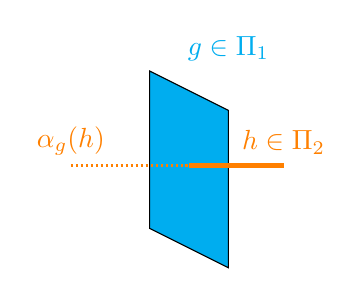
\begin{tikzpicture}
    \draw [yslant = -0.5, fill = cyan] (0,0) rectangle (1,2) (1,2.5)node[above , cyan] {$g\in\Pi_1 $};
    \draw[densely dotted, thick, orange] (-1,0.8) node[anchor = south] {$\alpha_{g}(h)$} -- (0.5,0.8)  ;
    \draw[ultra thick, orange] (0.5,0.8) -- (1.7,0.8) node[anchor = south]{$h\in \Pi_2$};
\end{tikzpicture}
\end{center}
穿过 $0$-形式对称性的生成元 $U_g$ 之后，$1$-形式对称性元素按 $h\mapsto \alpha_g(h)=g\rhd h$ 改变。

$\beta$ 的信息则编码在 $1$-形式缺陷的融合之中。
\begin{center}
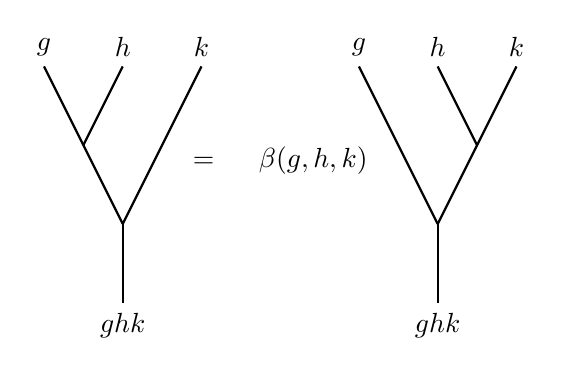
\begin{tikzpicture}[scale = 0.5]
    \draw[thick] (0,0) -- (2,-4) (0,0) node[above] {$g$};
    \draw[shift = {(8,0)} ,thick] (0,0) -- (2,-4) (0,0) node[above] {$g$};
    \draw[thick] (4,0) -- (2,-4) (4,0) node[above]{$k$}; 
    \draw[shift = {(8,0)}, thick] (4,0) -- (2,-4) (4,0) node[above]{$k$}; 
    \draw[thick] (2,-4) -- (2,-6) (2,-6) node[below]{$ghk$};
    \draw[shift = {(8,0)}, thick] (2,-4) -- (2,-6) (2,-6) node[below]{$ghk$};
    \draw[thick] (2,0) -- (1,-2) (2,0) node[above]{$h$};
    \draw[thick] (10,0) -- (11,-2) (10,0) node[above]{$h$} (6,-3) node[above]{$= \ \ \ \ \beta(g,h,k)$} ;
    
\end{tikzpicture}
\end{center}

上述从左到右的过程，按照共形场论中融合规则的叫法，有时称为 F-移动（F-move）。经过一次 F-移动之后，会出现 $1$-形式对称性的一个新生成元 $\beta(g,h,k)$。

弱 2-群的背景规范场为：$0$-形式对称性的 $A$ 与 $1$-形式对称性的 $B$。用单纯集（平坦联络）的语言来说，
\begin{enumerate}
    \item 对 $0$-形式部分，跃迁函数 $A_{ij}\in C^1(M,\Pi_1)$，而 $1$-上闭链条件要求对每个 2-单纯形 $\{ ijk\}$ 有
    \be A_{ij}A_{jk}A_{ki} = {\rm id}_{\Pi_1}  \ee
    
    \item 对 $1$-形式部分，规范场 $B\in C^2(M,\Pi_2)$ 满足一个扭曲-平移的上闭链条件
    \be\ba
    \delta_A B &= A^* \beta \\
    \Leftrightarrow \alpha_{A_{ij}} (B_{jkl}) B_{ikl}^{-1} B_{ijl} B_{ijk}^{-1} &= \beta(A_{ij},A_{jk},A_{kl})
    \ea\ee
    称之为“扭曲的”，是因为微分 $\delta_A$ 比通常的 Čech 微分 $\delta$ 多了一个 $\Pi_1$-作用；称之为“平移的”，是因为它不等于 0，而是等于 Postnikov 不变量。
\end{enumerate}

规范变换应当保持平坦性条件。这里有两类规范变换：
\begin{enumerate}
    \item 第一类是
    \be A \mapsto A , \ \ B\mapsto B + \delta_A \Lambda  \ee
    $A$ 场保持不变，$B$ 被平移一个扭曲恰当项。
    \item 第二类更为复杂，
    \be\ba 
    A_{ij} &\mapsto A^f_{ij} = f_i A_{ij} f_j^{-1} \\   
    B&\mapsto \alpha_f(B) + \xi(A,f) , \\ 
    \xi(A,f) \in C^2(M,\Pi_2) \ \ &{\rm and} \ \delta_{A^f}\xi(A,f) = A^{f*} B-\alpha_f (A^*\beta) \ .
    \ea\ee
\end{enumerate}

\begin{yizhu}
式 $\delta_A B = A^*\beta$ 的扭曲-平移条件极易写错符号与次序：展开为
$\alpha_{A_{ij}}(B_{jkl})B_{ikl}^{-1}B_{ijl}B_{ijk}^{-1}=\beta(A_{ij},A_{jk},A_{kl})$，
其中 $\alpha_{A_{ij}}(B_{jkl})$ 表示 $\Pi_1$ 通过 $\alpha$ 作用在 $\Pi_2$ 上（即交叉模的 Peiffer 作用）。
核对时请注意：$\delta_A$ 的下标 $A$ 指用 $0$-形式联络 twist 通常的 Čech 微分；若把 $\alpha$ 的作用方向记反，
得到的 Postnikov 类会差一个逆。
\end{yizhu}

\begin{yizhu}
第二类规范变换中的 $\xi(A,f)$ 不是自由参数：它必须满足 $\delta_{A^f}\xi = A^{f*}B-\alpha_f(A^*\beta)$，
这正是“平坦性在规范变换下保持”的要求。作者未展开此式的推导；其实质是：$B\mapsto \alpha_f(B)+\xi$ 之后，
要求 $\delta_{A^f}B'=A^{f*}\beta$，再与 $\delta_{A^f}\alpha_f(B)$ 的定义比较即得。
\end{yizhu}

% ==== 原文 PDF 第 62 页 ====
凝聚态系统中自然出现的 2-群结构之一是“对称性富化的规范理论”（symmetry-enriched gauge theory），
它可以看作对称性富化拓扑（SET）态的特例\cite{etingof2010fusion,PhysRevB.87.155115,PhysRevB.87.165107,Chang_2015,PhysRevB.93.155121,PhysRevB.94.235136,PhysRevB.96.115107,PhysRevB.100.115147,10.21468/SciPostPhys.8.2.028,PhysRevB.106.115104}。

例如，考虑一个 $(2+1)$ 维系统，其阿贝尔规范群为 $A$、对称群为 $\Pi_1$。$A$ 规范理论的任意子（激发）由规范群 $A$ 的量子双重（quantum double）描述。在阿贝尔情形，这对应于 $A\times\hat{A}$，其中 $A$ 与 $\hat{A}=\text{Hom}(A,U(1))$ 分别描述 $A$ 规范理论中的规范通量与规范荷。这类任意子的世界线可理解为 $1$-形式对称性 $\Pi_2=A\times\hat{A}$ 的拓扑缺陷线（TDL）。另一方面，$0$-形式对称性 $\Pi_1$ 正是通过作用 $\alpha$ 作用在任意子上。

2-群理论的全部数据与相容性条件，都可追溯到 SET 态的分类数据与障碍\cite{etingof2010fusion,PhysRevB.100.115147,wang2021domain}。更一般地，若考虑非阿贝尔的 $A$，则作为 $1$-形式对称性的量子双重 $\Pi_2=DA$ 将是非可逆的。于是 SET 态将对应于具有非可逆 $1$-形式对称性与可逆 $0$-形式对称性的系统；这两类对称性的相互作用会使分类变得更加复杂\cite{etingof2010fusion,PhysRevB.100.115147}。2-规范理论的格点模型可以写成离散非线性 $\sigma$-模型，这一表示来自把时空三角剖分为与 2-群相伴的分类空间，详见文献~\cite{PhysRevB.100.045105}。

% ==== 原文 PDF 第 63 页 ====
\subsection{例：带 't Hooft 反常的规范化}
\label{sec:2-group-gauging}

这里给出弱 2-群对称性的一个物理应用。

考虑一个 3 维量子场论，其 $0$-形式整体对称为 $\hat{\Pi}_2\times \Pi_1$，其中暂时取 $\hat{\Pi}_2$ 为阿贝尔群。该系统具有由下式描述的混合 't Hooft 反常：
\be S = 2\pi \int_{M_4} C\cup A^*\beta  \ee
其中 $C$ 是 $\hat{\Pi}_2$ 的背景 $1$-形式规范场，$A$ 是 $\Pi_1$ 的背景 $1$-形式规范场，$\beta$ 是 Postnikov 类。存在 't Hooft 反常时，我们无法对完整的 $\hat{\Pi}_2\times \Pi_1$ 对称性作规范化；但在对 $\hat{\Pi}_2$ 作规范化之后，可以得到一个新的 $1$-形式对称性 $\Pi_2\cong {\rm Hom}(\hat{\Pi}_2,U(1))$ 及相应的 $2$-形式背景规范场 $B$。

完成上述步骤后，新的拓扑作用量为
\be S = 2\pi \int_{M_3} C\cup B  + 2\pi \int_{M_4} C\cup A^*\beta \ee
它应当在 $\Pi_2$ 规范变换下规范不变，于是要求
\be  \delta B + A^* \beta = 0 \ee
这与我们先前给出的弱 2-群定义一致（若仔细看，会差一个符号约定）。因此在该理论中，$\Pi_1$、$\Pi_2$ 构成一个 2-群对称性 $(\Pi_1,\Pi_2,1,\beta)$，其中 $1$ 表示平凡作用。

\begin{yizhu}[原文疑误]
作者在此明言“差一个符号约定”（up to a sign notation, if you watch carefully），但未说明符号来源。
通常的约定是 $\delta B + A^*\beta = 0$ 与 $\delta_A B = A^*\beta$ 之间相差 $B\mapsto -B$ 的重新定义；
两种写法描述的 2-群相同，但若与文献直接比对公式，须先统一 $B$ 的符号约定。
\end{yizhu}

% ==== 原文 PDF 第 64 页 ====
\subsection{推广：弱 $n$-群}
\label{sec:n-group}
正如前面所说，“相等”这一条件总可以放松为“等价”，而描述这种等价关系所用的语言各有不同。

我们当然可以想象弱 $n$-群的草图：存在 $n$-态射，用来填补具有相同源与靶的两个 $(n-1)$-态射之间的空隙，如此逐级下降直到 $1$-态射。不过这里我们想描述的是一个相对简单的情形，它只是前一个例子的平凡推广。

回忆命题~\ref{prop:gauge}：当我们对一个 $p$-形式对称性作规范化时，将得到一个 $(d-p-2)$-形式对称性。现在考虑在 $(n+1)$ 维时空中、对完整的 $\hat{\Pi}_2\times \Pi_1$ 中的 $0$-形式对称性 $\hat{\Pi}_2$ 作规范化，设 't Hooft 反常用
\be  S = 2\pi \int_{M_{n+2}} C\cup A^*\beta   \ee
描述，其中 $\beta\in H^{n+1}(\Pi_1,\Pi_2)$ 是 Postnikov 类。这一特殊版本的弱 $n$-群中，$\Pi_1$ 是描述 $1$-态射的 $0$-形式对称性，$\Pi_2$ 是描述 $n$-态射的 $(n-1)$-形式对称性。

\subsection{非可逆对称性一瞥}
\label{sec:non-invertible}
本讲义中遇到的广义对称性都是可逆对称性，可以用群或高群描述。更广泛的一类对称性是非可逆对称性，其中包括更一般的高阶范畴对称性。对这类对称性，拓扑生成元服从一般的融合规则
\be
U_g(M)U_h(M)=\sum_i U_{g_i}(M_i)
\ee
而不是群的结合律。注意右端甚至可以由定义在维数各不相同的流形 $M_i$ 上的拓扑算符组成。非可逆对称性的研究领域发展迅速，感兴趣的读者可参阅近期讲义\cite{Schafer-Nameki:2023jdn}。

从凝聚态物理的角度看，$2+1$ 维拓扑序中非阿贝尔任意子的产生算符，可以解释为非可逆对称性的生成元。该对称性能够作用在 $1+1$ 维边界上，从而对可能的边界理论施加非可逆的对称性约束\cite{PhysRevResearch.2.043086,kong_mathematical_2020,kong_mathematical_2021,PhysRevResearch.2.033417,ji2022unified,PhysRevB.107.155136,PhysRevB.108.075105}。

我们给出 $d$ 维 $Spin(4N)$ 杨–米尔斯理论的一个例子\cite{Bhardwaj:2022yxj}。该理论具有 $\mb{Z}_2^{(1)}\times\mb{Z}_2^{(1)}$ 的 $1$-形式中心对称性，其背景 $2$-形式规范场记为 $B_2$ 与 $C_2$；此外还有 $D_{2N}$ 根系的一个 $\mb{Z}_2^{(0)}$ 外自同构，其背景规范场为 $A_1$。$\mb{Z}_2^{(0)}$ 对称性作用在 $D_{2N}$ 的 Dynkin 图上为

\begin{center}
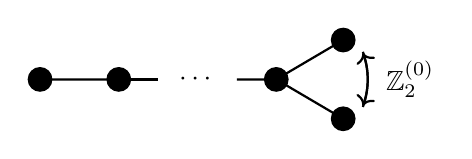
\begin{tikzpicture}
    \filldraw[] (0,0) circle (0.15) (1,0) circle (0.15) (3,0) circle (0.15) (3.85,0.5) circle (0.15) (3.85,-0.5) circle (0.15);
    \draw[thick] (0,0)--(1,0) (2.5,0)--(3,0) (3,0)--(3.85,0.5) (3,0)--(3.85,-0.5);
    \draw[thick] (1,0)--(1.5,0) node[anchor = west]{\textbf{$ \ \cdots$}};
    \draw[thick,->] (4.1,-0.35) arc (-20:20:1);
    \draw[thick,->] (4.1,0.35) arc (20:-20:1);
    \node[] at (4.7,0){$\bbZ_2^{(0)}$};
\end{tikzpicture}
\end{center}
它把 $D_{2N}$ 的表示 $\mbf{R}$ 映为其复共轭表示 $\overline{\mbf{R}}$。现在，在以 $B_2$ 为背景规范场对 $\mb{Z}^{(1)}$ 对称性作规范化之后，我们得到 $SO(4N)$ 杨–米尔斯理论，其混合 't Hooft 反常为
\be
\mc{A}=\pi\int_{M_{d+1}} A_1\cup C_2\cup \hat{B}_{d-2}
\ee
其中 $\hat{B}_{d-2}$ 是 $(d-3)$-形式对偶对称性的背景规范场。

最后，若进一步对 $A_1$ 与 $\hat{B}_{d-2}$ 作规范化，我们将得到带非可逆对称性缺陷的 $Pin^+(4N)$ 理论。

一般而言，若一个非可逆对称性来自这类部分规范化，则称为\textbf{非内禀的非可逆对称性}（non-intrinsically non-invertible symmetry）；否则称为\textbf{内禀的非可逆对称性}（intrinsically non-invertible symmetry）。

\begin{yizhu}
本节的 $Spin(4N)$ 例子是“非内禀非可逆对称性”的标准范例：它来自对 $SO(4N)$ 理论的 $\mathbb{Z}_2^{(1)}\times\mathbb{Z}_2^{(1)}$ 中心对称性作部分规范化。核对时请注意：
$\hat{B}_{d-2}$ 是 $(d-3)$-形式对偶对称性的背景场，其形式次数为 $d-2$，与 $A_1\cup C_2$（$1+2=3$ 次）相乘后总次数为 $d+1$，恰好是 $M_{d+1}$ 上的反常作用量所要求的次数。
\end{yizhu}

% ==== 原文 PDF 第 65--66 页 ====
\section*{致谢}

我们感谢 Lakshya Bhardwaj、Chi-Ming Chang、Max Hubner、Ruizhi Liu、Sakura Schafer-Nameki、Fajie Wang、Jingxiang Wu 与 Yi Zhang 就相关课题的讨论。我们也感谢北京大学听众的讨论与提问。QRW 由中国国家自然科学基金资助（批准号 12274250）。YNW 由中国国家自然科学基金（批准号 12175004）、北京大学启动经费（批准号 7100603667）以及中国科协青年人才托举工程（2022QNRC001）资助。


% ============================ 附录 ============================
\appendix
% ============================================================
% 片段：s06  对应原文 appendix1.tex 第 1--105 行；PDF 第 66--68 页
% 内容：附录 A  Čech 上同调
% 译者：lead   审校状态：初稿
% ============================================================

% ==== 原文 PDF 第 66 页 ====
\section{Čech 上同调}

\begin{keytakeaways}
  \begin{itemize}[leftmargin=1.4em,itemsep=2pt,topsep=2pt]
    \item \textbf{物理图像}：Čech 上同调把“如何在流形上一致地给连线赋群元素”这一物理问题（平坦联络、和乐）翻译成纯组合数据：坐标卡是 0-单纯形、交集是 1-单纯形、多重交集是高维单纯形。
    \item \textbf{数学工具}：良覆盖、单纯形、边缘算子 $\ptl$、链复形；以及由预层、限制映射 $\mathrm{Res}$ 与上边缘 $\delta$ 构成的 Čech 上链复形。
    \item \textbf{关键结论}：物理上关心的平坦联络局部数据满足 $A_{ij}A_{jk}A_{ki}=\mathrm{id}$ 之类的上闭链条件，而“不一致性”（如离散挠类）正是由 $H^k(\mathcal{U},\mathcal{F})$ 的非平凡类刻画。这为正文第 2.4 节的“平坦联络”视角提供了严格框架，也是后文 2-群背景场的 twisted/shifted 上闭链条件的语言基础。
  \end{itemize}
\end{keytakeaways}

\label{App:Cech}

本附录说明如何建立一种方法，把群元素妥善地赋给流形中的连线，即如平坦联络（见第~\ref{para:flatconn}~段）所描述的那样。

在流形的构造中，大家熟知的做法是用局部欧氏空间 $\bbR^n$ 的坐标卡（patch）之并来描述流形 $M$，
并用一组跃迁函数 $f_{ij} : \phi_i(U_i\cap U_j)\to \phi_j(U_i\cap U_j)$ 把它们粘合起来。
下面我们选取一个良覆盖（good cover），其中所有交集 $U_{ij}$ 都是单连通的，且同构于 $\bbR^n$。

Čech（上）同调本质上是一种借用坐标卡交集来定义（上）同调的方法。其构造如下：
\begin{enumerate}
    \item 每个 $U_i$ 代表一个 0-单纯形；
    \item 每个 $U_{ij} \equiv U_i\cap U_j$ 代表一个 1-单纯形；
    \item 每个 $k$-单纯形表示为
    \be 
    U_{i_0,\cdots , i_k} \equiv \bigcap_{m = 0}^k U_{i_m} \ ,
    \ee
    可用图表示为
    \begin{center}
        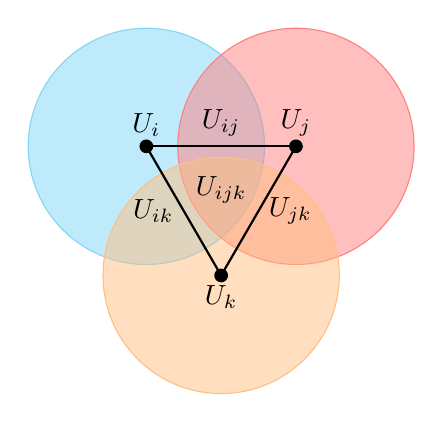
\begin{tikzpicture}
            \filldraw[ cyan!50,fill opacity=0.5 ] (0,0) circle (1.5) ; 
            \filldraw[] (0,0) circle (0.08);
            \filldraw[ red!50,fill opacity=0.5 ] (1.9,0) circle (1.5);
            \filldraw[] (1.9,0) circle (0.08);
            \filldraw[ orange!50,fill opacity=0.5 ] (0.95,-1.64) circle (1.5);
            \filldraw[] (0.95,-1.64) circle (0.08);

            \draw[thick]  (0,0)--(1.9,0)  ;
            \draw[thick]  (0.95,-1.64)--(1.9,0)   (1.425,-0.82)node[right]{$U_{jk}$};
            \draw[thick]  (0,0)--(0.95,-1.64)  (0.475, -0.82)node[left]{$U_{ik}$};
            \node[above] at (0,0) {$U_i$};
            \node[above] at (01.9,0) {$U_j$};
            \node[below] at (0.95,-1.64) {$U_k$};
            \node[above] at (0.95,0) {$U_{ij}$};
            \node[] at (0.95, -0.55) {$U_{ijk}$};
        \end{tikzpicture}
    \end{center}
    \item 边缘算子定义为\footnote{数学家可能会问加法结构从何而来。我们的说法是：现在工作在一个由 $U_{i_1,\cdots,i_k}$ 自由生成、系数取在 $\bbZ$ 中的阿贝尔群上（取其他阿贝尔群亦可）。}
    \be
    \ptl U_{i_0,\cdots ,i_k} = \sum_{m=0}^k (-1)^m U_{i_0,\cdots , \Hat{i}_m ,\cdots , i_k }
    \ee
    例如
    \be  \ptl U_{ijk} = U_{jk} -U_{ik} + U_{ij}  \ee
    图形上为
    \begin{center}
        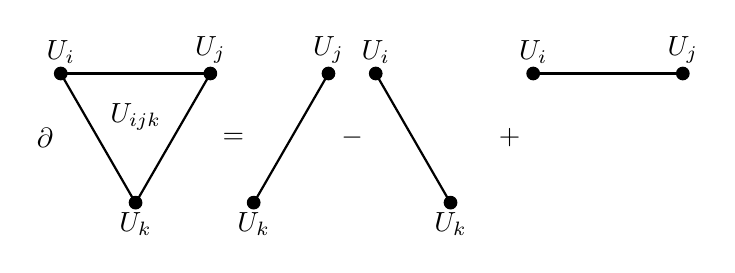
\begin{tikzpicture}
            \filldraw[] (0,0) circle (0.08);
            \filldraw[] (1.9,0) circle (0.08);
            \filldraw[] (0.95,-1.64) circle (0.08);

            \draw[thick] (0,0)--(1.9,0);
            \draw[thick,rotate = -60] (0,0)--(1.9,0);
            \draw[thick,rotate around = {60:(1.9,0)}] (1.9,0)--(0,0);
            \node[above] at (0,0) {$U_i$};
            \node[above] at (01.9,0) {$U_j$};
            \node[below] at (0.95,-1.64) {$U_k$};
            \node[] at (0.95, -0.55) {$U_{ijk}$};
            \node[] at (-0.2, -0.82){$\ptl$};
            \node[right] at (1.93, -0.82){$=$};


            
            \draw[shift = {(1.5,0)},thick,rotate around = {60:(1.9,0)}] (1.9,0)--(0,0);
            \draw[shift = {(4,0)},thick,rotate = -60] (0,0)--(1.9,0);
            \draw[shift = {(6,0)},thick] (0,0)--(1.9,0);
            \node[shift = {(4,0)},above] at (0,0) {$U_i$};
            \node[shift = {(6,0)},above] at (0,0) {$U_i$};

            \node[shift = {(1.5,0)},above] at (01.9,0) {$U_j$};
            \node[shift = {(6,0)},above] at (01.9,0) {$U_j$};

            \node[shift = {(4,0)},below] at (0.95,-1.64) {$U_k$};
            \node[shift = {(1.5,0)},below] at (0.95,-1.64) {$U_k$};
            \node[] at (3.7,-0.82) {$-$};
            \node[] at (5.7,-0.82) {$+$};

            \filldraw[shift = {(4,0)}] (0,0) circle (0.08);
            \filldraw[shift = {(1.5,0)}] (1.9,0) circle (0.08);
            \filldraw[shift = {(1.5,0)}] (0.95,-1.64) circle (0.08);
            \filldraw[shift = {(6,0)}] (0,0) circle (0.08);
            \filldraw[shift = {(6,0)}] (1.9,0) circle (0.08);
            \filldraw[shift = {(4,0)}] (0.95,-1.64) circle (0.08);

        \end{tikzpicture}
    \end{center}
    \item 容易验证，借助 $\ptl$ 算子我们得到一个 $\bbZ$-分次的链复形。记
    \be C_k(\mathcal{U}) = \bigoplus_{i_0 < i_1 < \cdots < i_k} \mathbb{Z}[U_{i_0} \cap \cdots \cap U_{i_k}] \ .  \ee
\end{enumerate}

以上是同调部分；我们更关心的是上同调部分——其中流形 $M$ 被映到各种系数中，成为我们珍视的场。我们希望场位形满足哪些性质呢？
\begin{enumerate}
    \item 场（至少是局部的）是截面 $\Gamma (U,F)$，其中 $F$ 是我们选定的某个参数空间。
    \item 为使截面映射既抽象又符合直觉，对 $V\subseteq U$ 应当存在限制映射 ${\rm Res}_{U,V} : \Gamma(U,F)\to \Gamma(V,F)$，使得
    \be  {\rm Res}_{U,U} = {\rm id}_{F} \ , \ \ \ {\rm Res}_{V,W} \circ {\rm Res}_{U,V} = {\rm Res}_{U,W} \ . \ee
    \item 对某些场，我们希望它们至少能在同一局部坐标卡上相加，即对每个 $U_i$，$\Gamma(U_i,F)$ 是一个阿贝尔群。
    于是限制映射至少应当尊重加法结构，使每个 ${\rm Res}_{U,V}$ 都是阿贝尔群同态：
    \be  {\rm Res}_{U,V} : {\rm Hom}_{\rm Ab} (\Gamma(U,F),\Gamma(V,F))  \ee
\end{enumerate}
上述语言概括起来就是：\textbf{我们想要的是 $M$ 上的阿贝尔群预层}，这种预层记作 $\mathcal{F}$。
于是，我们通过把每个 $p$-单纯形映为该单纯形上预层的一个元素，来定义一个 Čech $p$-上链 $C^p(M,\mathcal{U})$（$\CU$ 表示图册之集），即
\be
f : U_{i_1,\cdots, i_p} \mapsto G\in \CF ({U_{i_1,\cdots, i_p}})  
\ee
而微分算子 $\delta_p$ 由 ${\rm Res}$ 与 $\ptl$ 实现：对 $p$-上链，
\be
(\delta_p f)(\sigma ) = \sum_{k=0,p+1} (-1)^{k}  {\rm Res}_{\ptl_k \sigma, \sigma } (f ) (\ptl_k \sigma)   \ \
\ee
其中 $\sigma\in C^p(M,\CU)$，且 $\ptl_k (U_{i_1,\cdots,i_p}) \equiv U_{i_1,\cdots, \Hat{i}_k,\cdots,i_p} $。于是 Čech 上同调群定义为
\be  
H^k(\CU,\CF) \equiv \frac{{\rm ker}(\delta_k)}{{\rm im}(\delta_{k-1}) }  \ .
\ee

\begin{yizhu}
本附录中记号有一处容易混淆：$C_k(\mathcal{U})$（下标 $k$）是链复形中的链群，而 $C^p(M,\mathcal{U})$（上标 $p$）是上链群；
两者由预层 $\mathcal{F}$ 的截面给出。核对时请注意 $\delta_p$ 的指标：$\delta_p: C^p\to C^{p+1}$，
因此上同调 $H^k=\ker\delta_k/\operatorname{im}\delta_{k-1}$ 中分子分母的指标差一。
\end{yizhu}

\begin{yizhu}
原文在边缘算子求和中写作 $\sum_{k=0,p+1}$（逗号代替了范围符号），这是排版笔误，含义应为 $k=0,\dots,p+1$ 的求和；此处照原文保留。另，
“良覆盖”一词来自代数拓扑：要求覆盖的任意有限交集或为空、或可缩，才能保证 Čech 上同调与层上同调同构（Leray 定理）。
\end{yizhu}

% ============================================================
% 片段：s07  对应原文 appendix2.tex 第 1--20 行；PDF 第 68 页
% 内容：附录 B  群上同调
% 译者：lead   审校状态：初稿
% ============================================================

\section{群上同调}

\begin{keytakeaways}
  \begin{itemize}[leftmargin=1.4em,itemsep=2pt,topsep=2pt]
    \item \textbf{物理图像}：群上同调是“对称性在离散群上的反常与扩张”的统一语言：它把规范变换的闭合性/相容性表述为上闭链、把规范冗余表述为上边缘，从而把物理上的反常分类化为上同调群的计算。
    \item \textbf{数学工具}：$G$-模、$n$-上链群 $C^n(G,M)$、上边缘映射 $\delta_n$、上同调群 $H^n(G,M)$，以及与奇异上同调的同构 $H^n_{\rm grp}(G,A)\cong H^n_{\rm sing}(BG,A)$。
    \item \textbf{关键结论}：$H^3_{\rm grp}(\Pi_1,\Pi_2)$ 中的类就是正文第 5 节反复出现的 Postnikov 类 $\beta$ 的栖身之处；2-群的 Postnikov 数据 $(\Pi_1,\Pi_2,\alpha,\beta)$ 正是用它来刻画“$0$-形式对称性如何缠绕 $1$-形式对称性”。
  \end{itemize}
\end{keytakeaways}

\label{App:GrpChmlg}

群上同调是研究群及其作用的性质的数学工具。它是代数拓扑的一个分支，处理带有群作用的空间的上同调。
群系数在模中的上同调群定义如下。

设 $G$ 是一个群，$M$ 是一个 $G$-模。$G$ 以 $M$ 为系数的第 $n$ 个上同调群定义为商群
\[ H^n(G, M) = \frac{\text{ker}(\delta_n)}{\text{im}(\delta_{n-1})}, \]
其中 $\delta_n:H^n(G, M) \rightarrow H^{n+1}(G, M)$ 是由下式定义的上边缘映射：
\be\delta_n(f)(g_0, g_1, \ldots, g_n) = g_0f(g_1, \ldots, g_n) + \sum_{i=1}^{n}(-1)^if(g_0, \ldots, g_{i-1}g_i, \ldots, g_n) + (-1)^{n+1}f(g_0, \ldots, g_{n-1})\ee
这里 $f \in C^n(G, M)$，而 $C^n(G, M)$ 是 $G$ 以 $M$ 为系数的 $n$-上链群。

值得注意的是，有一个定理给出群上同调与奇异上同调之间的同构：
\be
H^n_{{\rm grp}}(G,A) \cong  H^n_{{\rm sing}}({\rm B}G,A) \ ,
\ee
其严格表述与证明可参见文献~\cite{weibel_1994}。

\begin{yizhu}
本附录的表述有一处不够严谨：$\delta_n$ 定义在 $n$-上链上，写作 $\delta_n:C^n(G,M)\to C^{n+1}(G,M)$，
而非原文所写的 $\delta_n:H^n\to H^{n+1}$（上边缘映射是上链层面的算子，$H^n$ 只是它诱导到商群上的映射）。
另请注意 $G$ 的作用是左作用，故上闭链条件中的 $g_0f(g_1,\dots)$ 表示用 $g_0$ 作用在系数上。
\end{yizhu}


% ============================ 参考文献 ============================
\input{refs.bbl}

\end{document}
